% Options for packages loaded elsewhere
\PassOptionsToPackage{unicode}{hyperref}
\PassOptionsToPackage{hyphens}{url}
%
\documentclass[
]{article}
\usepackage{amsmath,amssymb}
\usepackage{lmodern}
\usepackage{iftex}
\ifPDFTeX
  \usepackage[T1]{fontenc}
  \usepackage[utf8]{inputenc}
  \usepackage{textcomp} % provide euro and other symbols
\else % if luatex or xetex
  \usepackage{unicode-math}
  \defaultfontfeatures{Scale=MatchLowercase}
  \defaultfontfeatures[\rmfamily]{Ligatures=TeX,Scale=1}
\fi
% Use upquote if available, for straight quotes in verbatim environments
\IfFileExists{upquote.sty}{\usepackage{upquote}}{}
\IfFileExists{microtype.sty}{% use microtype if available
  \usepackage[]{microtype}
  \UseMicrotypeSet[protrusion]{basicmath} % disable protrusion for tt fonts
}{}
\makeatletter
\@ifundefined{KOMAClassName}{% if non-KOMA class
  \IfFileExists{parskip.sty}{%
    \usepackage{parskip}
  }{% else
    \setlength{\parindent}{0pt}
    \setlength{\parskip}{6pt plus 2pt minus 1pt}}
}{% if KOMA class
  \KOMAoptions{parskip=half}}
\makeatother
\usepackage{xcolor}
\usepackage[margin=1.0in]{geometry}
\usepackage{graphicx}
\makeatletter
\def\maxwidth{\ifdim\Gin@nat@width>\linewidth\linewidth\else\Gin@nat@width\fi}
\def\maxheight{\ifdim\Gin@nat@height>\textheight\textheight\else\Gin@nat@height\fi}
\makeatother
% Scale images if necessary, so that they will not overflow the page
% margins by default, and it is still possible to overwrite the defaults
% using explicit options in \includegraphics[width, height, ...]{}
\setkeys{Gin}{width=\maxwidth,height=\maxheight,keepaspectratio}
% Set default figure placement to htbp
\makeatletter
\def\fps@figure{htbp}
\makeatother
\setlength{\emergencystretch}{3em} % prevent overfull lines
\providecommand{\tightlist}{%
  \setlength{\itemsep}{0pt}\setlength{\parskip}{0pt}}
\setcounter{secnumdepth}{-\maxdimen} % remove section numbering
\newlength{\cslhangindent}
\setlength{\cslhangindent}{1.5em}
\newlength{\csllabelwidth}
\setlength{\csllabelwidth}{3em}
\newlength{\cslentryspacingunit} % times entry-spacing
\setlength{\cslentryspacingunit}{\parskip}
\newenvironment{CSLReferences}[2] % #1 hanging-ident, #2 entry spacing
 {% don't indent paragraphs
  \setlength{\parindent}{0pt}
  % turn on hanging indent if param 1 is 1
  \ifodd #1
  \let\oldpar\par
  \def\par{\hangindent=\cslhangindent\oldpar}
  \fi
  % set entry spacing
  \setlength{\parskip}{#2\cslentryspacingunit}
 }%
 {}
\usepackage{calc}
\newcommand{\CSLBlock}[1]{#1\hfill\break}
\newcommand{\CSLLeftMargin}[1]{\parbox[t]{\csllabelwidth}{#1}}
\newcommand{\CSLRightInline}[1]{\parbox[t]{\linewidth - \csllabelwidth}{#1}\break}
\newcommand{\CSLIndent}[1]{\hspace{\cslhangindent}#1}
\usepackage{upgreek}
\usepackage{booktabs}
\usepackage{longtable}
\usepackage{graphicx}
\usepackage{array}
\usepackage{multirow}
\usepackage{wrapfig}
\usepackage{float}
\usepackage{colortbl}
\usepackage{pdflscape}
\usepackage{tabu}
\usepackage{threeparttable}
\usepackage{threeparttablex}
\usepackage[normalem]{ulem}
\usepackage{makecell}
\usepackage{setspace}
\doublespacing
\usepackage[left]{lineno}
\linenumbers
\modulolinenumbers
\usepackage{helvet} % Helvetica font
\renewcommand*\familydefault{\sfdefault} % Use the sans serif version of the font
\usepackage[T1]{fontenc}
\usepackage[shortcuts]{extdash}
\usepackage[document]{ragged2e}
\ifLuaTeX
  \usepackage{selnolig}  % disable illegal ligatures
\fi
\IfFileExists{bookmark.sty}{\usepackage{bookmark}}{\usepackage{hyperref}}
\IfFileExists{xurl.sty}{\usepackage{xurl}}{} % add URL line breaks if available
\urlstyle{same} % disable monospaced font for URLs
\hypersetup{
  hidelinks,
  pdfcreator={LaTeX via pandoc}}

\author{}
\date{\vspace{-2.5em}}

\begin{document}

\raggedright

\hypertarget{waste-not-want-not-revisiting-the-analysis-that-called-into-question-the-practice-of-rarefaction}{%
\section{Waste not, want not: Revisiting the analysis that called into
question the practice of
rarefaction}\label{waste-not-want-not-revisiting-the-analysis-that-called-into-question-the-practice-of-rarefaction}}

\vspace{20mm}

\textbf{Running title:} Revisiting ``Waste not, want not''

\vspace{20mm}

Patrick D. Schloss\({^\dagger}\)

\vspace{40mm}

\({\dagger}\) To whom correspondence should be addressed:

\href{mailto:pschloss@umich.edu}{pschloss@umich.edu}

Department of Microbiology \& Immunology

University of Michigan

Ann Arbor, MI 48109

\vspace{20mm}

\textbf{Research article}

\newpage

\hypertarget{abstract}{%
\subsection{Abstract}\label{abstract}}

In 2014, McMurdie and Holmes published the provocatively titled, ``Waste
not, want not: why rarefying microbiome data is inadmissible''. The
claims of their study have significantly altered how microbiome
researchers control for the unavoidable uneven sequencing depths that
are inherent in modern 16S rRNA gene sequencing. Confusion over the
distinction between the definitions of rarefying and rarefaction
continues to cloud the interpretation of their results. More
importantly, the authors made a variety of choices in designing and
analyzing their simulations that were potentially problematic. I
identified 11 factors that could have compromised the results of the
original study. I reproduced the original simulation results and
assessed the impact of those 11 factors on the underlying conclusion
that rarefying data is inadmissible. Throughout, the design of the
original study made choices that caused rarefying and rarefaction to
appear to perform worse than they truly did. Most important were the
approaches used to assess ecological distances, the removal of samples
with low sequencing depth, and not accounting for conditions where
sequencing effort is confounded with treatment group. Although the
original study criticized rarefying for the arbitrary removal of valid
data, repeatedly rarefying data many times (i.e., rarefaction)
incorporates all the data. In contrast, it is the removal of rare taxa
that would appear to remove valid data. Overall, I show that rarefaction
is the most robust approach to control for uneven sequencing effort when
considered across a variety of alpha and beta diversity metrics.

\hypertarget{importance}{%
\subsubsection{Importance}\label{importance}}

Over the past 10 years, the best method for normalizing the sequencing
depth of samples characterized by 16S rRNA gene sequencing has been
contentious. An often cited paper by McMurdie and Holmes forcefully
argued that rarefying the number of sequence counts was ``inadmissible''
and should not be employed. However, I identified a number of problems
with the design of their simulations and analysis that could compromise
their results. In fact, when I reproduced and expanded upon their
analysis, it was clear that rarefaction was actually the most robust
approach for controlling for uneven sequencing effort across samples.
Rarefaction limits the rate of falsely detecting and rejecting
differences between treatment groups. Far from being ``inadmissible'',
rarefaction is a valuable tool for analyzing microbiome sequence data.

\newpage

\hypertarget{introduction}{%
\subsection{Introduction}\label{introduction}}

Microbiome studies that use amplicon sequencing to characterize multiple
samples use PCR to amplify 16S rRNA gene fragments using primers with
distinct barcodes or index sequences (1--3). These barcodes allow
researchers to pool PCR products and then deconvolute the resulting
sequence data based on the barcode sequences. Despite researchers' best
efforts to generate equimolar pools of PCR products, it is common to
observe more than 10-fold variation in the number of sequences per
sample (4). Researchers desire strategies to minimize uneven sequencing
depth and thus need methods to control for this unevenness in their
analyses. Of course, uneven sequencing is not unique to microbiome
research and is a challenge faced by all community ecologists (5, 6).
Common approaches to control for the effects of uneven sequencing depths
include use of proportional abundance (i.e., relative abundance),
scaling of counts, parameter estimation, and rarefaction (7--23).

In 2014 Paul McMurdie and Susan Holmes published ``Waste not, want not:
why rarefying microbiome data is inadmissible'' (WNWN) in \emph{PLOS
Computational Biology} (24). Their paper has had a significant impact on
the approaches that microbiome researchers use to analyze 16S rRNA gene
sequence data. According to Google Scholar, this paper has been cited
more than 2,400 times as of June 2023. There has been a rebuttal of WNWN
that showed how rarefaction is beneficial in some cases (25); however,
the proponents of WNWN appear to be holding sway over the microbiome
community. I have received correspondence from researchers over the past
10 years asking how to address critiques from reviewers who criticize my
correspondents' analysis for using rarefaction (e.g., see
\url{https://twitter.com/inanna_nalytica/status/1264299305067786242}). I
have also received similar comments from reviewers regarding my own
work. For example, I received the critique for a preprint that I posted
in 2020 that analyzed the practice of removing rare taxa from microbiome
analyses {[}see comments linked to (4);
\url{https://web.archive.org/web/20230308191505/http://dalmug.org/filter-review/}{]}.
In the process of responding to these reviewers' comments and preparing
a manuscript investigating rarefaction and other approaches to control
for uneven sequencing effort, I grew to appreciate that there is
significant confusion in the field over what is meant by ``rarefying''
and ``rarefaction''.

McMurdie and Holmes discussed and defined ``rarefying'' in WNWN
(citation numbers updated from the original to those of the current
study):

\begin{quote}
``Instead, microbiome analysis workflows often begin with an ad hoc
library size normalization by random subsampling without replacement, or
so-called rarefying (13, 26, 27). There is confusion in the literature
regarding terminology, and sometimes this normalization approach is
conflated with a non-parametric resampling technique --- called
rarefaction (5), or individual-based taxon re-sampling curves (28) ---
that can be justified for coverage analysis or species richness
estimation in some settings (28), though in other settings it can
perform worse than parametric methods (29). Here we emphasize the
distinction between taxon re-sampling curves and normalization by
strictly adhering to the terms rarefying or rarefied counts when
referring to the normalization procedure, respecting the original
definition for rarefaction. Rarefying is most often defined by the
following steps (13).

\begin{enumerate}
\def\labelenumi{\arabic{enumi}.}
\tightlist
\item
  Select a minimum library size, N\textsubscript{L,m}. This has also
  been called the rarefaction level (26), though we will not use the
  term here.
\item
  Discard libraries (microbiome samples) that have fewer reads than
  N\textsubscript{L,m}.
\item
  Subsample the remaining libraries without replacement such that they
  all have size N\textsubscript{L,m}.
\end{enumerate}

Often N\textsubscript{L,m} is chosen to be equal to the size of the
smallest library that is not considered defective, and the process of
identifying defective samples comes with a risk of subjectivity and
bias. In many cases researchers have also failed to repeat the random
subsampling step (3) or record the pseudorandom number generation
seed/process --- both of which are essential for reproducibility.''
\end{quote}

It was unfortunate that McMurdie and Holmes used the term ``rarefying''
in this quote and throughout their manuscript. The authors were correct
to state that the distinction between ``rarefying'' and ``rarefaction''
is confusing and leads to their conflation. Adding to the confusion is
that the papers cited in the first sentence of this quote (i.e., (13,
26, 27)) either do not use the words ``rarefy'' or ``rarefying'' or use
them interchangeably with ``rarefaction''. For example, Hughes and
Hellman did not use ``rarefy'' and use ``rarefaction'' in the
traditional sense with multiple subsamplings (13). Meanwhile, the
QIIME-based literature appears to use ``rarefy'' and ``rarefaction''
interchangeably to mean only a single subsampling (26, 27). Subsequent
researchers have continued to conflate the terms when citing WNWN
(\textbf{Supplemental Text}). An exemplar of the confusion is the
creation of a technique that uses ``repeatedly rarefying'' as an
approach distinct from rarefaction when they were re-proposing
traditional rarefaction (30).

As shown in the quoted text from WNWN, McMurdie and Holmes did emphasize
the distinction between rarefying and rarefaction. However, because they
seem to have coined a new definition for rarefying, they added to the
confusion by using the generally used verb form of rarefaction. Further
confusion comes from the author's admonition in the final sentence of
the above quoted text that some researchers have failed to repeat the
subsampling step. Traditionally, repeating the subsampling step a large
number of times and averaging the result is rarefaction (12, 13, 28). In
other words, rarefying or subsampling is rarefaction, but with a single
randomization. To minimize confusion, I will use ``subsampling'' in
place of ``rarefying'' through the remainder of this study.

For clarity, I will use the following definition of rarefaction:

\begin{enumerate}
\def\labelenumi{\arabic{enumi}.}
\tightlist
\item
  Select a minimum library size, N\textsubscript{L,m}. Researchers are
  encouraged to report the value of N\textsubscript{L,m}.
\item
  Discard samples that have fewer reads than N\textsubscript{L,m}.
\item
  Subsample the remaining libraries without replacement such that they
  all have size N\textsubscript{L,m}.
\item
  Compute the desired metric (e.g., richness, Shannon diversity,
  Bray-Curtis distances) using the subsampled data
\item
  Repeat steps 3 and 4 a large number of iterations (typically 100 or
  1,000). Researchers are encouraged to report the number of iterations.
\item
  Compute summary statistics (e.g., the mean) using the values from step
  4.
\end{enumerate}

This definition aligns with how rarefaction was originally defined for
comparing richness (i.e., the number of taxa in a community) across
communities when communities are sequenced to different depths (5, 6).
With this more general approach to the definition of rarefaction,
rarefaction can be performed using any alpha or beta diversity metric.
This strategy has been widely used by my research group and others and
is available in the mothur software package using commands such as
\texttt{summary.single}, \texttt{rarefaction.single},
\texttt{phylo.diversity}, and \texttt{dist.shared}. The procedure
outlined above could also be used for hypothesis tests of differential
abundance; however, consideration is needed to synthesize the results of
these tests across a large number of replications.

\hypertarget{description-and-critique-of-simulation-a-from-wnwn}{%
\subsection{Description and critique of ``Simulation A'' from
WNWN}\label{description-and-critique-of-simulation-a-from-wnwn}}

McMurdie and Holmes analyzed the effect of subsampling and other
approaches on clustering accuracy using what they called ``Simulation
A'' in their Figure 2A and elsewhere in WNWN. In Simulation A, they
investigated the ability to correctly assign simulated microbiome
samples to one of two clusters representing two simulated treatment
groups. Thankfully, the R code for Simulation A was provided by the
authors in the
\texttt{simulation-cluster-accuracy/simulation-cluster-accuracy-server.Rmd}
R-flavored markdown (R markdown) file that was published as Protocol S1
in WNWN. I will outline the simulation strategy below and will reference
line numbers from their R markdown file with ``L'' as a prefix.

For the WNWN cluster analysis, OTU abundance distributions for the two
treatment groups were generated using human fecal and ocean data
originally take from the GlobalPatterns dataset (L129) (2). To generate
the fecal and ocean distributions, the authors included any operational
taxonomic unit (OTU) that appeared in more than one of the 4 fecal and 3
ocean samples (L60 and L137). The OTUs were sorted by how many of the 7
samples the OTUs were observed in followed by their total abundance
across all 7 samples (L139). From this sorted list they obtained the
identifiers of the first 2,000 OTUs (L66). Returning to the 7 samples
they selected the data for the corresponding 2,000 OTUs and pooled the
OTU abundances of the fecal and ocean samples separately to create two
OTU abundance distributions (L144, L159-160, L197-198). Next, the fecal
and ocean distributions were mixed in 8 different fractions to generate
two community types that differed by varying effect sizes (i.e., 1.00,
1.15, 1.25, 1.50, 1.75, 2.00, 2.50, and 3.50; L170-195, L220); an effect
size of 1.00 generated a null model with no difference between the
treatment groups. To simulate the variation in sequencing depth across
the 80 samples, they normalized the number of sequences from each of the
26 samples in the GlobalPatterns dataset so that the median number of
sequences (Ñ\textsubscript{L}) across the samples had 1,000, 2,000,
5,000, or 10,000 sequences (L324-325). They then randomly sampled the 26
normalized sequencing depths, with replacement, to generate 80
sequencing depths. From each community type, they simulated 40 samples
by sampling to the desired number of sequences (L73, L230-233 and
L326-327). Each simulation condition was repeated 5 times (L85).
Finally, they removed rare and low prevalence OTUs in two steps. First,
they removed any OTUs whose total abundance was less than 3 across all
80 samples and that did not appear in at least 3 samples (L368-386).
Second, they removed any OTUs that did not have more than 1 sequence in
more than 5\% of the 80 samples (i.e., 4 samples) and that did not have
a total abundance across the 80 samples greater than one half of the
number of samples in each community type (i.e., 20) (L523-538, L551).
Simulation A consisted of 160 simulations (8 effect sizes x 4 median
sequencing depths x 5 replicates = 160 simulations).

After generating the OTU counts for the 160 simulations, the authors
applied several normalization methods, distance calculations, and
clustering algorithms to the data. To normalize the OTU data the WNWN
analysis either applied no normalization procedure (L559), calculated
OTU relative abundances (L392-401, L562-563), subsampled the data
(L409-416, L566-569), performed Variance Stabilization using the
\texttt{DESeq} R package (L478-504, L580-583)(7), or performed
Upper-Quartile Log-Fold Change normalization using the \texttt{edgeR} R
package (L425-457, L576-577, L622-721) (19). In subsampling the data,
the authors either included all of the samples or removed samples whose
sequencing depth fell below the 5, 10, 15, 20, 25, and 40 percentile
across all 80 samples (L96, L1065-1077).

Non-normalized data were used to calculate Bray-Curtis, Euclidean,
Poisson, and Weighted UniFrac distances (L793-798, L801-806). Relative
abundance data were used to calculate Bray-Curtis, Unweighted UniFrac ,
and Weighted UniFrac distances (L760-767). Subsampled data were used as
input to calculate distances between samples using Bray-Curtis,
Euclidean, Unweighted UniFrac, Weighted UniFrac distances, Poisson
distances, and top-Mean Squared Difference (L769-775, L793-798,
L801-806). DESeq Variance Stabilization normalized data were used to
calculate Bray-Curtis, Euclidean, and Weighted Unifrac distances
(L793-798). The Upper-Quartile Log-Fold Change normalized data were only
used to calculate top-Mean Squared Difference distances (L801-806). WNWN
calculated Bray-Curtis (31), Euclidean (31), Unweighted UniFrac (32),
and Weighted UniFrac distances (33) using the \texttt{Phyloseq} R
package (34). They calculated Poisson distances using the
\texttt{PoiClaClu} R package (35). The top-mean squared difference was
calculated using the \texttt{edgeR} R package (19). The resulting
distance matrices were used to cluster the 80 samples into one of two
clusters using partitioning around the medoid (PAM), K-means clustering,
and hierarchical clustering (L865-879). Although data for all three
methods were presented in Protocol S1, only the PAM data were presented
in the main manuscript. The accuracy of the clustering assignments was
quantified as the fraction of the 80 samples that were assigned to the
correct cluster (L887-908). Since some of the subsampling conditions
removed samples below a minimum sequencing depth threshold, those
samples were counted as mis-clustered samples yielding minimum
accuracies below 50\%.

Although all simulations represent an artificial representation of
reality and can be critiqued, I have identified eleven elements of the
design of Simulation A that warranted further review.

\begin{enumerate}
\def\labelenumi{\arabic{enumi}.}
\tightlist
\item
  Simulated conditions were only replicated 5 times each, potentially
  increasing the sensitivity of results to the choice of the random
  number generator seed
\item
  The average sizes of the libraries were small by modern standards,
  which may limit the generalizability of the results
\item
  DESeq-based Variance Stabilization generates negative values and was
  used with distance calculation methods that are sensitive to negative
  values, which likely led to nonsense distances and clusters
\item
  A single subsampling of each dataset was evaluated rather than using
  rarefaction, which likely resulted in noisier data
\item
  Results using PAM clustering were not directly compared to those of
  K-means and hierarchical clustering, although close inspection
  suggests that K-means may have been superior to PAM for some
  conditions
\item
  Subsampling removed the smallest 15\% of the samples, which penalized
  accuracy values by 15 percentage points
\item
  The distribution of library sizes was not typical of those commonly
  seen in microbiome analyses, which may limit the generalizability of
  the results
\item
  A filtering step was applied to remove rare taxa from the simulated
  datasets, which may have skewed the shape of the community
  distributions
\item
  There was no accounting for differences in performance when library
  sizes are confounded with treatment group
\item
  Clustering accuracy was used rather than the more direct and
  frequently applied comparisons of beta diversity using permutation
  tests
\item
  There was no consideration of effects of normalization methods on
  alpha diversity metrics, which is the traditional application of
  rarefaction
\end{enumerate}

Below, I replicated the original WNWN simulations and evaluated these
points to reassess whether subsampling or rarefaction are
``inadmissible''.

\hypertarget{results}{%
\subsection{Results}\label{results}}

\hypertarget{replication-of-wnwn-simulations-and-results}{%
\subsubsection{Replication of WNWN simulations and
results}\label{replication-of-wnwn-simulations-and-results}}

Before assessing the impact of the points I critiqued above, I attempted
to replicate the results shown in Figures 4 and 5 of WNWN using the
authors' code. I created a Conda environment that used the R version and
package versions that were as close as possible to those used in WNWN.
It was necessary to patch the WNWN's R markdown file to render the
document to be compatible with the overall workflow of this study. I was
able to generate figures similar to those presented as WNWN's Figures 4
and 5; my results are shown in this study as Figures 1 and 2,
respectively. The differences in results are likely due to differences
in software versions and operating systems. It is also worth noting that
the published versions of the two figures differ from those included in
Protocol S1 within the rendered HTML file
(\texttt{simulation-cluster-accuracy/simulation-cluster-accuracy-server.html})
and that the figure numbers are one higher in the paper than those
generated by the R markdown file (i.e., Protocol S1 labels the figures
as Figures 3 and 4 corresponding to the published Figures 4 and 5).
Regardless of the differences, my results were qualitatively similar to
that provided in WNWN's Protocol S1.

\hypertarget{simulated-conditions-were-only-replicated-5-times-each-potentially-increasing-the-sensitivity-of-results-to-the-choice-of-the-random-number-generator-seed}{%
\subsubsection{1. Simulated conditions were only replicated 5 times
each, potentially increasing the sensitivity of results to the choice of
the random number generator
seed}\label{simulated-conditions-were-only-replicated-5-times-each-potentially-increasing-the-sensitivity-of-results-to-the-choice-of-the-random-number-generator-seed}}

Each simulated condition was replicated 5 times in WNWN and the paper
reported the mean and standard deviation of the replicate clustering
accuracies. The relatively small number of replicates accounts for the
jerkiness of the lines in WNWN's Figures 4 and 5 (e.g.~the Bray-Curtis
distances calculated on the DESeqVS normalized data). A better approach
would have been to use 100 replicates as this would reduce the
dependency of the results on the random number generator's seed. By
increasing the number of replicates it was also possible to compare the
probability of falsely and correctly clustering samples from the same
and different treatment groups together (see points 10 and 11, below).
Because the accuracies were not symmetric around the mean accuracy
values the median and 95\% confidence intervals or interquartile range
should have been reported. To test the effect of increasing the number
of replicates, I pulled apart the code in
\texttt{simulation-cluster-accuracy/simulation-cluster-accuracy-server.Rmd}
into individual R and bash scripts that were executed using a Snakemake
workflow with the same Conda environment I used above. This was
necessary since the number of simulated conditions increased 20-fold
with the additional replicates. Such intense data processing was not
practical within a single R markdown document. Again, the observed
results were qualitatively similar to those generated using the single R
markdown file (Figures 3 and 4). The increased number of replications
resulted in smoother lines and allowed me to present empirical 95\%
confidence intervals. For all analyses in the remainder of this paper, I
used 100 randomized replicates per condition.

\hypertarget{the-average-sizes-of-the-libraries-were-small-by-modern-standards-which-may-limit-the-generalizability-of-the-results}{%
\subsubsection{2. The average sizes of the libraries were small by
modern standards, which may limit the generalizability of the
results}\label{the-average-sizes-of-the-libraries-were-small-by-modern-standards-which-may-limit-the-generalizability-of-the-results}}

In the 10 years since WNWN was published, sequencing technology has
advanced and sequence collections have grown considerably. For more
modern datasets, it would be reasonable to expect a median number of
sequences larger than 10,000 (see Table 1 of (4)). Therefore, I included
an additional median depth of sequencing of 50,000 sequences with WNWN's
four median sequencing depths (i.e., 1,000, 2,000, 5,000, 10,000).
Additional sequencing coverage would be expected to result in more
robust distance values since there would be more information represented
in the data. Indeed, the added sequencing depth showed higher accuracy
values at lower effect sizes for the combinations of normalization
methods and distance calculations (Figure 3). Increased sequencing
coverage also resulted in improved clustering accuracy for lower effect
sizes when the library size minimum quantile was decreased (Figure 4). I
will revisit the choice of the library size minimum quantile below.

\hypertarget{deseq-based-variance-stabilization-generates-negative-values-and-was-used-with-distance-calculation-methods-that-are-sensitive-to-negative-values-which-likely-led-to-nonsense-distances-and-clusters}{%
\subsubsection{3. DESeq-based Variance Stabilization generates negative
values and was used with distance calculation methods that are sensitive
to negative values, which likely led to nonsense distances and
clusters}\label{deseq-based-variance-stabilization-generates-negative-values-and-was-used-with-distance-calculation-methods-that-are-sensitive-to-negative-values-which-likely-led-to-nonsense-distances-and-clusters}}

Close comparison of WNWN's Figure 4 and my version (Figure 3) revealed
several difference between the two plots. First, in the WNWN analysis,
the accuracies for the Weighted UniFrac distances at the largest effect
size (i.e., 3.5) were 1.00 for median sequencing depths of 1,000, 2,000,
and 10,000. In my version of the analysis, the values for the same
sequencing depths were 1.00, 1.00, and 1.00, respectively. The 95\%
confidence interval for these accuracies spanned between 0.51 and 1.00.
Second, clustering accuracy for Bray-Curtis and Weighted UniFrac
distances calculated using DESeq Variance Stabilization normalized OTU
counts were different between the original and my simulation at smaller
effect sizes and had wide confidence intervals. Inspection of the DESeq
Variance Stabilization normalized OTU counts revealed that the method
resulted in negative values. It has been suggested that WNWW turned
negative DESeq normalized counts to zero (25); however, I was unable to
find code in \texttt{simulation-cluster-accuracy-server.Rmd} that made
this transformation. In fact, rendering the R markdown files in WNWN's
Protocol S1 generated warning messages when passing the DESeq normalized
counts to the Bray-Curtis calculator, which said, ``results may be
meaningless because data have negative entries in method `bray'\,''.
Although the Weighted UniFrac calculator function did not generate a
similar warning message, negative count values would also result in
similarly meaningless distances. Both are due to the fact that the
distance calculators sum the counts of each OTU in both samples being
compared. In contrast, a Euclidean distance does not use a similar sum,
but sums the square of the difference between the OTU abundance in each
sample. Even if negative values were converted to zeroes, this would
effectively the same as removing rare taxa, which could have a
significant impact on the shape of the communities (4). To assess the
prevalence of negative counts in the simulated data, I quantified the
fraction of negative values in the OTU matrix from each simulation and
counted the number of simulations where the normalized OTU table had at
least one negative value (Figure 5). In general the fraction of negative
OTU counts increased with effect size, but decreased with sequencing
effort. The fraction of simulations with at least one negative value
increased with effect size and sequencing effort. The high frequency of
negative OTU counts resulted in highly variable Bray-Curtis and Weighted
UniFrac values. It is likely that because the WNWN analysis only used 5
replicates that the large variation in accuracies at high effect sizes
was missed initially. For the rest of this reanalysis study, I will only
report results using the DESeq-based Variance Stabilization
normalization with the Euclidean distance.

\hypertarget{a-single-subsampling-of-each-dataset-was-evaluated-rather-than-using-rarefaction-which-likely-resulted-in-noisier-data}{%
\subsubsection{4. A single subsampling of each dataset was evaluated
rather than using rarefaction, which likely resulted in noisier
data}\label{a-single-subsampling-of-each-dataset-was-evaluated-rather-than-using-rarefaction-which-likely-resulted-in-noisier-data}}

A more robust analysis would have used rarefaction since it would have
averaged across a large number of random subsamplings (e.g., 100 or
1,000). By using a large number of subsamplings the likelihood of
incorporating all of the OTUs would have increased. Rather than being
guilty of ``omission of available valid data'' as claimed in WNWN, with
a sufficient number of subsamplings, traditional rarefaction uses all of
the available data. To fairly compare subsampling, as employed in WNWN,
and rarefaction, I removed the 15\% of samples with the lowest number of
sequences and compared the clustering accuracies from a single
subsampling to rarefaction with 100 randomizations. This analysis
revealed two benefits of rarefaction. First, the median distances
generated by rarefaction was always at least as large as those from a
single subsample (Figure 6). The difference was most pronounced for
smaller average library sizes and at smaller effect sizes. The
Unweighted UniFrac distances were most impacted by the use of
rarefaction over subsampling. Second, the interquartile ranges in
clustering accuracy by rarefaction were generally smaller than those by
subsampling and showed similar trends to the difference in the median
distances (Figure 6). Because rarefaction incorporates more of the data
and generally performed better than subsampling, the remainder of this
analysis will report results using rarefaction rather than by
subsampling, except when noted.

\hypertarget{results-using-pam-clustering-were-not-directly-compared-to-those-of-k-means-and-hierarchical-clustering-although-close-inspection-suggests-that-k-means-may-have-been-superior-to-pam-for-some-conditions}{%
\subsubsection{5. Results using PAM clustering were not directly
compared to those of K-means and hierarchical clustering, although close
inspection suggests that K-means may have been superior to PAM for some
conditions}\label{results-using-pam-clustering-were-not-directly-compared-to-those-of-k-means-and-hierarchical-clustering-although-close-inspection-suggests-that-k-means-may-have-been-superior-to-pam-for-some-conditions}}

The clustering accuracy measurements reported in the body of WNWN were
determined using PAM-based clusters while Protocol S1 also includes
K-means and hierarchical clustering. Although the data were not
displayed in a manner that lent itself to direct comparison in Protocol
S1, close inspection of the rendered figures suggested that PAM may not
have been the optimal choice in all situations. Actually, K-means
clustering appeared to perform better in many simulations. Because the
accuracies were the smallest at lower effect sizes, I focused my
comparison at the effect size of 1.15. For each set of 100 replicated
simulated datasets, I compared the clustering accuracy across clustering
methods to see how often each clustering method resulted in the highest
accuracy (Figure 7). Indeed, K-means clustering performed better than
the other methods. Among all combinations of normalization methods,
distance calculations, and read depths, K-means clustering was at least
as good as the other methods in 74.39\% of the randomizations (Figure
7); PAM clustering resulted in clustering accuracies as good or better
than the other methods in 49.92\% of the randomizations; and
hierarchical clustering (HClust) was at least as good as the other
methods for 44.32\% of the randomizations. Finally, I specifically
compared the clustering accuracies using rarefaction for each of the
distance calculations methods using PAM and K-means clustering. Among
the 30 combinations of distance calculations and read depths, K-means
performed better than PAM in 29 cases with PAM doing better in the 1
other case (i.e., calculating distances with Euclidean using 10,000
sequences). When using subsampled data, K-means clustering performed
better than PAM in each case. Because K-means clustering did so much
better than PAM clustering in the simulated conditions, I used K-means
clustering for the remainder of this study.

\hypertarget{subsampling-removed-the-smallest-15-of-the-samples-which-penalized-accuracy-values-by-15-percentage-points}{%
\subsubsection{6. Subsampling removed the smallest 15\% of the samples,
which penalized accuracy values by 15 percentage
points}\label{subsampling-removed-the-smallest-15-of-the-samples-which-penalized-accuracy-values-by-15-percentage-points}}

In WNWN, the authors quantified the tradeoff between median sequencing
depth, the number of samples removed below the threshold, and clustering
accuracy (WNWN's Figure 5, my Figure 4). Although the optimal threshold
varied by distance metric, normalization method, and sequencing depth,
they removed samples whose number of sequences was less than the 15th
percentile (L404-419). They acknowledged that this screening step, which
was only used with subsampling, would decrease clustering accuracy
putting it at a relative disadvantage to the other methods (page 5,
column 1, last paragraph). Therefore, it was not surprising that the
peak clustering accuracy for their subsampled data was at 85\%. Because
the true best threshold would not known \emph{a priori} in an actual
microbiome study, it would be impossible for researchers to conduct a
sensitivity analysis comparing the tradeoffs between sequencing depth,
sample number, and clustering accuracy to select a sequencing depth for
their analysis without the risk of p-hacking. The differences in
clustering accuracy between subsampling and rarefaction with PAM and
K-means clustering indicated that it was necessary to reassess the
tradeoff between the library size minimum quantile and clustering
accuracy. When using rarefaction, K-means clustering, and only
considering conditions with 2,000 or more sequences, there was not a
condition where setting a higher threshold resulted in a better accuracy
than using all of the samples (Figure 8). These results showed that for
modern sequencing depths, using the full datasets with rarefaction and
K-means clustering resulted in accuracies that were better than those
observed when removing the smallest 15\% of the samples from each
simulated dataset. When the WNWN Figure 4 was recast with these
approaches, rarefaction performed at least as well as any of the other
transformations with each distance calculation (Figure 9).

\hypertarget{the-distribution-of-library-sizes-was-not-typical-of-those-commonly-seen-in-microbiome-analyses-which-may-limit-the-generalizability-of-the-results}{%
\subsubsection{7. The distribution of library sizes was not typical of
those commonly seen in microbiome analyses, which may limit the
generalizability of the
results}\label{the-distribution-of-library-sizes-was-not-typical-of-those-commonly-seen-in-microbiome-analyses-which-may-limit-the-generalizability-of-the-results}}

As described above, the sequencing depths used in the 26 GlobalPatterns
datasets were used as the distribution to create sequencing depths for
the 80 samples that were generated in each simulation. The
GlobalPatterns datasets had a mean of 1,085,256.8 sequences and a median
of 1,106,849 sequences per dataset (Figure 10). The datasets ranged in
sequencing depth between 58,688 and 2,357,181 sequences for a 40.16-fold
difference. Rather than representing a typically observed distribution
of sequencing depths that would be skewed right (see Figure S1 from
(4)), the sequencing depth distribution was normally distributed
(Shapiro-Wilk test of normality, P=0.57). From these simulations it is
unclear how sensitive the various normalizations and distance
calculations were to a more realistic skewed distribution. A second
limitation of this sequencing depth distribution is that it only
contained 26 unique sequencing depths such that each sequencing depth
would have been re-used an average of 3.08 times in each simulation.
Yet, it is unlikely for a real sequence collection to have duplicate
sequencing depths. To reassess the WNWN results in the context of a more
typical distribution of sequencing depths, I created a new set of
simulations to test the effect of the shape of the distribution on the
results. I created a simple sequencing depth distribution where there
were 80 depths logarithmically distributed between the minimum and
maximum sequencing depths of the GlobalPatterns dataset (Figure 10). The
median of this distribution was 372,040 and the mean was 629,824.8. When
I regenerated the WNWN's Figures 4 and 5 using the log-scaled sequencing
effort distribution, the differences in normalization methods were more
apparent (Figure 11 and 12). For each of the distance calculators,
rarefaction to the size of the smallest dataset yielded accuracies that
were at least as good as the other methods across effect sizes and
median sequencing depths. The difference was most pronounced at smaller
effect sizes and sequencing depths. When comparing the performance of
rarefaction across distance calculators for different effect sizes,
sequencing depths and size of smallest sample, the accuracies I observed
using the log-scaled sample sizes was at least as good as those obtained
using the GlobalPatterns-based distribution (Figure 9).

\hypertarget{a-filtering-step-was-applied-to-remove-rare-taxa-from-the-simulated-datasets-which-may-have-skewed-the-shape-of-the-community-distributions}{%
\subsubsection{8. A filtering step was applied to remove rare taxa from
the simulated datasets, which may have skewed the shape of the community
distributions}\label{a-filtering-step-was-applied-to-remove-rare-taxa-from-the-simulated-datasets-which-may-have-skewed-the-shape-of-the-community-distributions}}

McMurdie and Holmes were emphatic that ``\textbf{rarefying biological
count data is statistically inadmissible} because it requires the
omission of available valid data'' (emphasis in original). Thus it is
strange that they argue against removing data when
rarefying/subsampling, but accept removing rare and low-prevalence OTUs
prior to normalizing their counts. This practice has become common in
microbiome studies and is the standard approach in tools such as Dada2,
Unoise, and Deblur (36--39). However, my previous work has shown that
rare sequences from a poorly sequenced sample often appear in more
deeply sequenced samples suggesting that they are not necessarily
artifacts (4). Furthermore, removing rare sequences alters the structure
of communities and has undesirable effects on downstream analyses.
Although my previous work does an extensive analysis of the effects of
removing rare sequences, I wanted to explore the effect of filtering in
the context of the WNWN simulation framework. For each of the filtered
and non-filtered OTU tables I calculated the the difference in accuracy
between replicates for each normalization method and distance calculator
across effect sizes for a Ñ\textsubscript{L} of 10,000 (Figure 13). The
median difference in accuracies (i.e.~clustering accuracies with
filtered data minus those without filtering) did not deviate
meaningfully from zero. However, the 95\% confidence intervals were most
pronounced at large effect sizes when using raw counts, DESeq Variance
Stabilization and Upper-Quartile Log-Fold Change and at smaller effect
sizes when using rarefaction and relative abundances. Given the large
variation caused by removing rare taxa and my previous work, OTU
filtering should not be performed in microbiome analyses. Considering
the minimal effect that removing rare OTUs had on the median difference
in clustering accuracy in the current simulation framework, I have used
the filtered datasets throughout the current study.

\hypertarget{there-was-no-accounting-for-differences-in-performance-when-library-sizes-are-confounded-with-treatment-group}{%
\subsubsection{9. There was no accounting for differences in performance
when library sizes are confounded with treatment
group}\label{there-was-no-accounting-for-differences-in-performance-when-library-sizes-are-confounded-with-treatment-group}}

I and others have observed that not using rarefaction can lead to
falsely detecting differences between communities when sequencing effort
is confounded with the treatment group (25, 40). Previous analyses
showed that in these situations rarefaction did the best job of
controlling the rates of false detection (i.e., Type I errors) and
maintaining the statistical power to detect differences (i.e., 1-rate of
Type II errors) of differences between groups of samples. Such
situations have been observed when comparing communities at different
body parts where one site is more likely to generate contaminating
sequence reads from the host (e.g., 41). To determine whether this
result was replicated with the WNWN simulation framework, I created a
sequencing depth distribution where sequencing depth was fully
confounded with the treatment group using both the GlobalPatterns and
Log-scaled sequence distributions. To confound the sequencing depth,
sequencing depths from one treatment group were drawn from below the
median number of sequences of the sequencing distribution and those for
the second treatment group were from above the median. To assess the
risk of falsely detecting clusters, I compared the clustering accuracies
using an effect size of 1.00 using both the confounded and randomized
sequencing distributions (see rows 1 and 2 of Figure 14). The samples
should have only been assigned to one cluster; however, each of the
clustering methods forced the samples into two clusters. So, when there
are two groups of 40 samples that do not differ, the best a method could
do would be to correctly assign 41 of the 80 samples for an accuracy of
0.51. The false detection risk did not vary by method when the
sequencing depth was randomized across treatment groups. Yet, when the
sequencing depth was confounded with treatment group, rarefaction was
the most consistent normalization method for controlling the generation
of spurious clusters. At larger effect sizes the ability to correctly
identify two clusters increased when the sequencing depth was confounded
with treatment group (Figure 14). At the effect size of 1.15, the
rarefied data generated the highest accuracy clusters regardless of
whether the sequencing depths were confounded. Although the level of
confounding in this simulation was extreme, it highlights the ability of
rarefaction to control the false detection rate and the ability to
correctly detect clusters relative to the other normalization methods.

\hypertarget{clustering-accuracy-was-used-rather-than-the-more-direct-and-frequently-applied-comparisons-of-beta-diversity-using-permutation-tests}{%
\subsubsection{10. Clustering accuracy was used rather than the more
direct and frequently applied comparisons of beta diversity using
permutation
tests}\label{clustering-accuracy-was-used-rather-than-the-more-direct-and-frequently-applied-comparisons-of-beta-diversity-using-permutation-tests}}

Since WNWN was published, there has been controversy over the use of
clustering methods to group samples (i.e., enterotypes). Concerns have
been raised including whether such clustering should be done on
ecological distances or sequence counts and the biological
interpretation of such clusters (27, 42, 43). As described in the
previous point, one notable challenge with using clustering accuracy as
the dependent variable is that the clustering methods force the samples
into one of two clusters. For the case where the effect size was 1.00,
it was impossible for all 80 samples to be assigned to a single cluster.
A more commonly used approach for analyzing distance matrices is to use
a non-parametric analysis of variance test (i.e., AMOVA, PERMANOVA,
NP-ANOVA)(44). I subjected each of the distance matrices to such a test
using \texttt{adonis2}, a function from the \texttt{vegan} R package
that implements this test to assess the effects of each normalization
and distance calculation method on the Type I errors and statistical
power (45). When sequencing depths were randomly distributed across the
two treatment groups, the Type I error did not meaningfully deviate from
the expected 5\% (Figure 15). However, when sequencing depths were
confounded with treatment group, rarefaction was the only normalization
approach to control the Type I error. Similar to the clustering accuracy
results, when distances were calculated using rarefaction, the tests
consistently had the best statistical power (Figure 15). When
considering both Type I error and power, rarefaction performed the best
among the different normalizations.

\hypertarget{there-was-no-consideration-of-effects-of-normalization-methods-on-alpha-diversity-metrics-which-is-the-traditional-application-of-rarefaction}{%
\subsubsection{11. There was no consideration of effects of
normalization methods on alpha diversity metrics, which is the
traditional application of
rarefaction}\label{there-was-no-consideration-of-effects-of-normalization-methods-on-alpha-diversity-metrics-which-is-the-traditional-application-of-rarefaction}}

Rarefaction was originally proposed as a method for controlling uneven
sequencing effort when comparing community richness values (5, 6). Thus
it was surprising that WNWN did not consider the effect of the proposed
normalizations on alpha-diversity metrics such as richness or Shannon
diversity. Therefore, for each of the normalizations, I compared the
richness and diversity of the two treatment groups. The DESeq Variance
Stabilization normalized data were not included because the
normalization produced negative values which were not compatible with
calculations of richness or Shannon diversity. Also, data from the
Upper-Quartile Log-Fold Change normalization were not used for richness
calculations since the normalization returned the same richness values
for each sample regardless of the treatment group. I assessed whether
the alpha diversity was significantly different between the treatment
groups for each iteration using the non-parametric Wilcoxon two-sampled
test. I compared the risk of committing Type I errors and the power to
detect differences by the different normalizations (Figures 16 and 17).
For these analyses, I used the GlobalPatterns data with the random and
confounded distribution of sequencing depths. Similar to the results in
points 9 and 10, with the exception of rarefaction, the simulations
using a confounded sequence depth distribution resulted in all of the
replicates having a significant test. The power to detect differences in
richness and diversity at effect sizes of 1.15 and greater with
rarefaction was at least as high as any of the other normalizations.

One odd result from this analysis was that the power to detect
differences in richness at small effect sizes increased between 1,000 to
2,000 sequences with values of 0.91 and 1.00, respectively. The power
then decreased with increasing sequencing effort to 0.57 with 50,000
sequences. This appeared to be because although the parent distributions
had very different shapes, they shared a large number of rare taxa. When
using rarefaction to compare the distributions at the size of the
smallest distribution (i.e., 3,598,077 sequences), the feces parent
distribution had and average of 1,559.65 OTUs and the ocean had an
average of 1,335.00 OTUs; they shared an average of 894.66 OTUs.
However, when comparing the distributions at 1,000 and 50,000 sequences,
the Ocean distribution had greater richness than the feces distribution
by 43.76 and 6.05, respectively. Therefore, although more replicates at
lower effect sizes yielded a significant p-value at shallow rather than
deeper sequencing depths for richness, the direction of the difference
in richness was incorrect. This result underscores the challenges of
using metrics based on presence-absence data like richness and Jaccard
and Unweighted UniFrac distances to compare microbial communities.

\hypertarget{discussion}{%
\subsection{Discussion}\label{discussion}}

The conclusions from WNWN have had a lasting impact on how researchers
analyze microbiome sequence data. As I have demonstrated using WNWN's
simulation framework, their claims are not supported. The most important
points that lead to the difference in our conclusions include the choice
of clustering algorithm and arbitrarily selecting a sequencing effort
threshold that was used to remove samples. Furthermore, the decision to
evaluate the effectiveness of normalization methods based on clustering
samples adds a layer of analysis that has been controversial and not
widely used. Ultimately, the authors choice of the word ``rarefying''
has sewn confusion in the field because it is often used in place of the
word ``rarefaction''. As I have demonstrated there were numerous choices
throughout the original study that resulted in rarefying/subsampling
looking worse than it truly is. In fact, when the data of the current
study are taken as a whole, rarefaction is the preferred approach. Short
of obtaining the exact same number of sequences from each sample,
rarefaction remains the best approach to control for uneven sequencing
effort when analyzing alpha and beta diversity metrics. Although beyond
the scope of the current study, the same principles would also support
using rarefaction to control for uneven sequencing effort when
calculating alpha and beta diversity metrics in shotgun metagenomic
sequencing analyses.

Beyond the discussion of whether rarefaction is appropriate for
analyzing microbiome data it is worth commenting on WNWN's advice to use
DESeq's Variance Stabilization or edgeR's Upper-Quartile Log-fold Change
normalization strategies. These methods have been adopted from gene
expression analysis to microbiome analysis. Gene expression analysis
implicitly assumes that all samples have the same genes. While this
might work in comparing healthy and diseased tissues from a cohort of
patients, it does not generalize to those patients' microbiota.
Microbial populations are highly patchy in their distribution. Thus, a
zero count for gene expression is more likely to represent a gene below
the limit of detection whereas a zero count for a microbiome analysis is
more likely to represent the true absence of the OTU. In fact, zeroes
are less common in gene expression analyses. But because microbiome
studies have so many zeroes, it is necessary to add a pseudo-count to
all OTUs for both the edgeR and DESeq-based normalizations (L443 and
L487, respectively). In WNWN, a pseudo-count of 1 was used. However,
this value is arbitrary and the results can vary based on the choice of
pseudo-count and the patchiness of the communities being analyzed. Since
WNWN was published, compositional approaches have been proposed to
account for uneven sequencing and to provide improved interpretability
(14, 16--18, 46, 47). However, these methods also often require the use
of pseudo-counts and are not actually insensitive to uneven sequencing
(40). Rarefaction is preferred to these alternatives.

The choice of distance metric is a complicated question and the use of
six different metrics in WNWN illustrates the challenges of selecting
one. Within the ecology literature, Euclidean distances are widely
avoided because joint absence is weighted the same as joint presence of
taxa (31). As discussed in point 11, distances that are based on
community membership (i.e., the presence or absence of taxa) performed
worse than those than those that were based on community structure
(i.e., their relative abundance). For this reason, the Unweighted
UniFrac and other distances like the Jaccard or Sorenson distance
coefficients should likely be avoided. The Poisson distance metric is
largely novel to the microbial ecology literature and performed no
better than the more traditional distances. In the current analysis, the
phylogenetic Weighted UniFrac distance performed comparably to
Bray-Cutis distances for clustering or differentiating between
communities with \texttt{adonis2}. Regardless of the distance
calculation employed, they all performed best when using rarefaction
relative to the other normalization methods.

Although the authors claim that ``Rarefying counts requires an arbitrary
selection of a library size minimum that affects downstream inference''
(page 8, column 1, point 3), in actual microbiome studies the selection
of a sequencing depth is not as arbitrary as the authors claim. Rather,
to avoid p-hacking, researchers pick a set of criteria where they will
include or exclude samples prior to testing their data. Examples of
criteria might include the presence of a large gap in the sequencing
effort distribution, a desire to include poorly sequenced controls, or
the \emph{a priori} stipulation of a minimum sequencing effort. To
mitigate concerns of arbitrary or engineered minimum library sizes,
researchers should indicate the rationale for the threshold they
selected.

WNWN performed a second set of simulations to address the effect of
normalization method on the ability to correctly detect differential
abundance of OTUs that were randomly selected to have their relative
abundances changed (i.e., ``Simulation B''). Re-addressing this set of
simulations is beyond the scope of the current analysis and others have
already contributed critiques (25). However, many of the same concerns
addressed above would apply. Perhaps most important is the fact that if
the relative abundance of several OTUs increase, then the relative
abundance of all other OTUs would necessarily decrease because the data
are compositional (47). Thus, one would expect every OTU to be
differentially abundant. Because of this, it is not possible to truly
modify the abundance of a set of OTUs independent of all other OTUs.
This is an important limitation of tests of methods attempting to detect
differentially abundant OTUs. Regardless, a form of rarefaction could
still be employed for detecting differential abundance. One could
subsample the data, perform the statistical test, and identify the
differentially abundant OTUs. This process could be repeated and the
results synthesized. In my experience the largest differences between
subsamples are for low relative abundances OTUs, which are unlikely to
be statistically significant.

In a parallel set of analyses I have used alternative simulation and
evaluation strategies to look more closely at rarefaction and its
alternatives (40) and the practice of filtering low abundance sequences
(4). The results of those studies are similar to this analysis. These
studies demonstrate that it is actually sequence and OTU filtering that
``requires the omission of available valid data'' and that rarefaction
is the only available method for controlling the effects of uneven
sequencing. Far from being inadmissible, rarefaction of unfiltered
datasets yields the most robust results.

\hypertarget{methods}{%
\subsection{Methods}\label{methods}}

\hypertarget{code-availability}{%
\subsubsection{Code availability}\label{code-availability}}

A git repository containing all of the code needed to reproduce this
study is available at
\url{https://www.github.com/SchlossLab/Schloss_WNWN_XXXXX_2023}. All
simulations and analyses were performed using R and bash scripts using
Snakemake (v7.24.0) to track dependencies and automate the pipeline and
Conda (v4.12.0) and mamba (v1.1.0) to specify software and package
versions (see \texttt{workflow/envs/nr-base.yml} in the repository).
This manuscript was written as an R markdown document and rendered using
the \texttt{rmarkdown} R package (v2.18). All figures were generated
using \texttt{dplyr} (v1.1.0) and \texttt{ggplot2} (v3.4.2) from the
\texttt{tidyverse} metapackage (v1.3.2) and \texttt{ggtext} (v0.1.2) and
\texttt{ggh4x} (v0.2.4) within R (v.4.2.2; see
\texttt{workflow/envs/nr-modern.yml} in the repository).

\hypertarget{reproducing-wnwn-protocol-s1}{%
\subsubsection{Reproducing WNWN Protocol
S1}\label{reproducing-wnwn-protocol-s1}}

The compressed directory published with WNWN as Protocol S1 is available
on the \emph{PLOS Computational Biology} website with WNWN at
\url{https://doi.org/10.1371/journal.pcbi.1003531.s001}. To render the R
markdown files to HTML files using software and packages as similar as
possible to that of WNWN, I created an environment (see
\texttt{workflow/envs/nr-s1.yml} in this study's repository) that
contained versions as close to those indicated in the pre-rendered
files. The most important packages for the reproduction of the cluster
analysis included \texttt{DESeq} (my version: v1.39.0 vs.~WNWN version:
v1.14.0), \texttt{edgeR} (v3.30.0 vs.~v3.4.0), \texttt{cluster} (v2.1.0
vs v1.14.4), \texttt{phyloseq} (v1.32.0 vs.~v1.6.0), and
\texttt{PoiClaClu} (v1.0.2.1 vs.~1.0.2). In addition, I used R v4.0.2
whereas the WNWN analysis used v3.0.2. Finally, to render the
\texttt{simulation-cluster-accuracy-server.Rmd} file to HTML, it was
necessary to apply a patch to the code. This patch set the path to the
location where the figures should be saved and removed the R code that
deleted all objects in the environment. Both changes were necessary to
better organize the project and had no substantial bearing on the
content of the rendered HTML file.

\hypertarget{simulated-communities}{%
\subsubsection{Simulated communities}\label{simulated-communities}}

The code contained within
\texttt{simulation-cluster-accuracy-server.Rmd} was spilt into
individual R scripts and modified to make the generation of the
simulated communities more modular and scalable. The code for generating
the simulated communities was run using the \texttt{nr-s1} Conda
environment. The ocean and feces parent distributions were generated as
described above. Five variables were altered to simulate each set of
communities. First, eight mixing fractions were used to manipulate the
effect size between the two simulated treatment groups with 40 samples
per group. These were the same effect sizes used in the WNWN study (1.00
{[}i.e., no difference{]}, 1.15, 1.25, 1.50, 1.75, 2.00, 2.50, and
3.50). Second, the number of sequences in each of the 80 samples was
either randomly selected from the 26 library sizes contained within the
GlobalPatterns dataset or from a log distribution of 80 sequencing
depths evenly distributed between the most shallow (58,688 sequences)
and deeply (2,357,181 sequences) sequenced samples in the GlobalPatterns
dataset (Figure 10). Third, the resulting 80 sequencing depths were
scaled so that the median sequencing depth across the 80 samples was
either 1,000, 2,000, 5,000, 10,000, or 50,000 sequences. Fourth, the
sequencing depth of each sample was either randomly assigned to each
treatment group or assigned so that those depths less than or greater
than the median were assigned to separate treatment groups. Finally,
each set of conditions was replicated 100 times. These five parameters
resulted in 1,600 simulated datasets (8 effect sizes x 2 sequencing
depth models x 5 sequencing depths x 2 sequencing depth assignment
models x 100 replicates).

\hypertarget{generation-of-distances-between-communities}{%
\subsubsection{Generation of distances between
communities}\label{generation-of-distances-between-communities}}

Next, each simulation was further processed by filtering rare OTUs, to
normalize uneven sequencing depths, and to calculate ecological
distances between samples. Again, the code contained within
\texttt{simulation-cluster-accuracy-server.Rmd} was spilt into
individual R scripts and modified to make the generation of the
simulated communities more modular and scalable within the
\texttt{nr-s1} Conda environment. First, each simulation was either
filtered to remove rare OTUs or left unfiltered. As was done in the WNWN
study, filtering was performed in two steps: (1) any OTUs whose total
abundance was less than 3 across all 80 samples and that did not appear
in at least 3 samples and (2) any OTU that did not have more than 1
sequence in more than 5\% of the 80 samples (i.e., 4 samples) and that
did not have a total abundance across the 80 samples greater than one
half of the number of samples in each community type (i.e., 20) were
removed. Second, OTU data was normalized by one of six approaches: (1)
non-normalized raw counts, (2) relative abundance, (3) DESeq Variance
Stabilization, (4) Upper-Quartile Log-Fold Change normalization using
edgeR, (5) a single subsampling to a common number of sequences, (6)
rarefaction with 100 randomizations to a common number of sequences.
Although the data were not presented, the WNWN code and my code also
normalized the counts using trimmed mean of M-values (TMM) and relative
log expression (RLE) in edgeR. The level of subsampling and rarefaction
was selected based on the size of the sample whose sequencing depth was
at the 0 (i.e., included all of the samples), 5, 10, 15, 20, 25, and
40th percentiles. Finally, the normalized simulated datasets were used
to calculate pairwise distances between the 80 samples using seven
different calculations: Bray-Curtis, Euclidean, Poisson, Mean Squared
Difference, Unweighted UniFrac, Weighted Unifrac, and Biological
Coeffcient of Variation (BCV); however, data using BCV were not
discussed in this or the WNWN analysis. For the rarefaction normalized
data, each of the 100 subsampled datasets were used to calculate a
distance matrix. The mean of the 100 distance matrices was used as the
distance matrix for the rarefaction data. As indicated in the Results
section, there were combinations of normalization and distance methods
that were not compatible (e.g., DESeq Variance Stabilization
normalization with Bray-Curtis distances). In such cases, distance
matrices were coded as \texttt{NA}. My choice of combinations of
normalizations and distances to visualize was determined by the WNWN
analysis except where noted. For each simulated dataset there were 280
possible combinations of filtering, normalization, and distance methods
(2 filtering methods x 20 normalization methods x 7 distance methods).

\hypertarget{analysis-of-distances-between-communities}{%
\subsubsection{Analysis of distances between
communities}\label{analysis-of-distances-between-communities}}

Two general strategies were used to analyze the pairwise distances in
each distance matrix. First, by recycling the the code contained within
\texttt{simulation-cluster-accuracy-server.Rmd} in the \texttt{nr-s1}
Conda environment, samples were assigned to one of two clusters using
partitioning around the medoid (PAM) with the \texttt{pam} function from
the \texttt{cluster} R package, K-means clustering with the
\texttt{kmeans} function from the \texttt{stats} base R package, and
hierarchical clustering with the \texttt{hclust} and \texttt{cutree}
functions from the \texttt{stats} base R package. The accuracy of the
clustering was measured as the fraction of the 80 samples assigned to
the correct cluster. As in WNWN, if samples were removed because the
number of sequences in them fell below the threshold for subsampling or
rarefaction, then the accuracy could be below 50\%. For the effect size
of 1.00, all of the samples should have been assigned to one group;
however, because they were forced into two groups there would be 41
``correctly'' assigned samples of the 80 samples (i.e., an accuracy of
0.51). Second, the distance matrices were analyzed for significant
different centroids using the \texttt{adonis2} function from the
\texttt{vegan} package (v2.6-4) in the \texttt{nr-modern} Conda
environment. The fraction of significant tests was the fraction of the
100 replicate simulations that had a p-value less than or equal to 0.05.
The Type I error rate for a condition was the fraction of significant
tests when the effect size was 1.00. The power was the fraction of
significant tests at other effect sizes.

\hypertarget{analysis-of-richness-and-diversity-between-communities}{%
\subsubsection{Analysis of richness and diversity between
communities}\label{analysis-of-richness-and-diversity-between-communities}}

Using the \texttt{nr-s1} Conda environment, I measured the richness and
Shannon diversity using the normalized OTU counts. Richness was measured
by counting the number of OTUs for each sample across the simulations
and the Shannon diversity using their relative abundance using the
commonly used formula (31). For the rarefaction data, each of the 80
samples in the 100 subsampled datasets were used to calculate the
richness and diversity. The mean across the 100 subsamplings was used as
the value for the rarefaction data across each of the 80 samples. To
assess differences between the two treatment groups, the richness and
diversity values were compared using the two-sample Wilcoxon
non-parametric test with the \texttt{wilcox.test} from the
\texttt{stats} base R package. Similar to the analysis using
\texttt{adonis2}, the fraction of significant tests was the fraction of
the 100 replicate simulations that had a p-value less than or equal to
0.05. The Type I error rate for a condition was the fraction of
significant tests when the effect size was 1.00. The power was the
fraction of significant tests at other effect sizes.

\hypertarget{acknowledgements}{%
\subsection{Acknowledgements}\label{acknowledgements}}

I am grateful to Dr.~Paul McMurdie and Dr.~Susan Holmes for publishing
the source code that they used to conduct their analysis as R markdown
files in the supplement to WNWN. It would not have been possible for me
to replicate and build upon their simulations without their code.

\newpage

\hypertarget{references}{%
\subsection{References}\label{references}}

\setlength{\parindent}{-0.25in}
\setlength{\leftskip}{0.25in}

\noindent

\hypertarget{refs}{}
\begin{CSLReferences}{0}{1}
\leavevmode\vadjust pre{\hypertarget{ref-Sogin2006}{}}%
\CSLLeftMargin{1. }%
\CSLRightInline{\textbf{Sogin ML}, \textbf{Morrison HG}, \textbf{Huber
JA}, \textbf{Welch DM}, \textbf{Huse SM}, \textbf{Neal PR},
\textbf{Arrieta JM}, \textbf{Herndl GJ}. 2006. Microbial diversity in
the deep sea and the underexplored {``}rare biosphere{''}. Proceedings
of the National Academy of Sciences \textbf{103}:12115--12120.
doi:\href{https://doi.org/10.1073/pnas.0605127103}{10.1073/pnas.0605127103}.}

\leavevmode\vadjust pre{\hypertarget{ref-Caporaso2010}{}}%
\CSLLeftMargin{2. }%
\CSLRightInline{\textbf{Caporaso JG}, \textbf{Lauber CL},
\textbf{Walters WA}, \textbf{Berg-Lyons D}, \textbf{Lozupone CA},
\textbf{Turnbaugh PJ}, \textbf{Fierer N}, \textbf{Knight R}. 2010.
Global patterns of 16S {rRNA} diversity at a depth of millions of
sequences per sample. Proceedings of the National Academy of Sciences
\textbf{108}:4516--4522.
doi:\href{https://doi.org/10.1073/pnas.1000080107}{10.1073/pnas.1000080107}.}

\leavevmode\vadjust pre{\hypertarget{ref-Kozich2013}{}}%
\CSLLeftMargin{3. }%
\CSLRightInline{\textbf{Kozich JJ}, \textbf{Westcott SL}, \textbf{Baxter
NT}, \textbf{Highlander SK}, \textbf{Schloss PD}. 2013. Development of a
dual-index sequencing strategy and curation pipeline for analyzing
amplicon sequence data on the {MiSeq} illumina sequencing platform.
Applied and Environmental Microbiology \textbf{79}:5112--5120.
doi:\href{https://doi.org/10.1128/aem.01043-13}{10.1128/aem.01043-13}.}

\leavevmode\vadjust pre{\hypertarget{ref-Schloss2023sing}{}}%
\CSLLeftMargin{4. }%
\CSLRightInline{\textbf{Schloss PD}. 2020. Removal of rare amplicon
sequence variants from 16S {rRNA} gene sequence surveys biases the
interpretation of community structure data. bio{R}xiv.
doi:\href{https://doi.org/10.1101/2020.12.11.422279}{10.1101/2020.12.11.422279}.}

\leavevmode\vadjust pre{\hypertarget{ref-Sanders1968}{}}%
\CSLLeftMargin{5. }%
\CSLRightInline{\textbf{Sanders HL}. 1968. Marine benthic diversity: A
comparative study. The American Naturalist \textbf{102}:243--282.
doi:\href{https://doi.org/10.1086/282541}{10.1086/282541}.}

\leavevmode\vadjust pre{\hypertarget{ref-Hurlbert1971}{}}%
\CSLLeftMargin{6. }%
\CSLRightInline{\textbf{Hurlbert SH}. 1971. The nonconcept of species
diversity: A critique and alternative parameters. Ecology
\textbf{52}:577--586.
doi:\href{https://doi.org/10.2307/1934145}{10.2307/1934145}.}

\leavevmode\vadjust pre{\hypertarget{ref-Anders2010}{}}%
\CSLLeftMargin{7. }%
\CSLRightInline{\textbf{Anders S}, \textbf{Huber W}. 2010. Differential
expression analysis for sequence count data. Genome Biology
\textbf{11}:R106.
doi:\href{https://doi.org/10.1186/gb-2010-11-10-r106}{10.1186/gb-2010-11-10-r106}.}

\leavevmode\vadjust pre{\hypertarget{ref-Beule2020}{}}%
\CSLLeftMargin{8. }%
\CSLRightInline{\textbf{Beule L}, \textbf{Karlovsky P}. 2020. Improved
normalization of species count data in ecology by scaling with ranked
subsampling (SRS): Application to microbial communities. PeerJ
\textbf{8}:e9593.
doi:\href{https://doi.org/10.7717/peerj.9593}{10.7717/peerj.9593}.}

\leavevmode\vadjust pre{\hypertarget{ref-Chao2003}{}}%
\CSLLeftMargin{9. }%
\CSLRightInline{\textbf{Chao A}, \textbf{Shen T-J}. 2003. Environmental
and Ecological Statistics \textbf{10}:429--443.
doi:\href{https://doi.org/10.1023/a:1026096204727}{10.1023/a:1026096204727}.}

\leavevmode\vadjust pre{\hypertarget{ref-Chao2016}{}}%
\CSLLeftMargin{10. }%
\CSLRightInline{\textbf{Chao A}, \textbf{Chiu C-H}. 2016.
\href{https://doi.org/10.1002/9781118445112.stat03432.pub2}{Species
richness: Estimation and comparison}, p. 1--26. \emph{In} Wiley
StatsRef: Statistics reference online. John Wiley \& Sons, Ltd.}

\leavevmode\vadjust pre{\hypertarget{ref-Costea2014}{}}%
\CSLLeftMargin{11. }%
\CSLRightInline{\textbf{Costea PI}, \textbf{Zeller G}, \textbf{Sunagawa
S}, \textbf{Bork P}. 2014. A fair comparison. Nature Methods
\textbf{11}:359--359.
doi:\href{https://doi.org/10.1038/nmeth.2897}{10.1038/nmeth.2897}.}

\leavevmode\vadjust pre{\hypertarget{ref-Hughes2001}{}}%
\CSLLeftMargin{12. }%
\CSLRightInline{\textbf{Hughes JB}, \textbf{Hellmann JJ},
\textbf{Ricketts TH}, \textbf{Bohannan BJM}. 2001. Counting the
uncountable: Statistical approaches to estimating microbial diversity.
Applied and Environmental Microbiology \textbf{67}:4399--4406.
doi:\href{https://doi.org/10.1128/aem.67.10.4399-4406.2001}{10.1128/aem.67.10.4399-4406.2001}.}

\leavevmode\vadjust pre{\hypertarget{ref-Hughes2005}{}}%
\CSLLeftMargin{13. }%
\CSLRightInline{\textbf{Hughes JB}, \textbf{Hellmann JJ}. 2005.
\href{https://doi.org/10.1016/s0076-6879(05)97017-1}{The application of
rarefaction techniques to molecular inventories of microbial diversity},
p. 292--308. \emph{In} Methods in enzymology. Elsevier.}

\leavevmode\vadjust pre{\hypertarget{ref-Lin2020}{}}%
\CSLLeftMargin{14. }%
\CSLRightInline{\textbf{Lin H}, \textbf{Peddada SD}. 2020. Analysis of
microbial compositions: A review of normalization and differential
abundance analysis. npj Biofilms and Microbiomes \textbf{6}:60.
doi:\href{https://doi.org/10.1038/s41522-020-00160-w}{10.1038/s41522-020-00160-w}.}

\leavevmode\vadjust pre{\hypertarget{ref-Love2014}{}}%
\CSLLeftMargin{15. }%
\CSLRightInline{\textbf{Love MI}, \textbf{Huber W}, \textbf{Anders S}.
2014. Moderated estimation of fold change and dispersion for {RNA}-seq
data with {DESeq}2. Genome Biology \textbf{15}:550.
doi:\href{https://doi.org/10.1186/s13059-014-0550-8}{10.1186/s13059-014-0550-8}.}

\leavevmode\vadjust pre{\hypertarget{ref-Martino2019}{}}%
\CSLLeftMargin{16. }%
\CSLRightInline{\textbf{Martino C}, \textbf{Morton JT}, \textbf{Marotz
CA}, \textbf{Thompson LR}, \textbf{Tripathi A}, \textbf{Knight R},
\textbf{Zengler K}. 2019. A novel sparse compositional technique reveals
microbial perturbations. {mSystems} \textbf{4}:00016--19.
doi:\href{https://doi.org/10.1128/msystems.00016-19}{10.1128/msystems.00016-19}.}

\leavevmode\vadjust pre{\hypertarget{ref-Paulson2013}{}}%
\CSLLeftMargin{17. }%
\CSLRightInline{\textbf{Paulson JN}, \textbf{Stine OC}, \textbf{Bravo
HC}, \textbf{Pop M}. 2013. Differential abundance analysis for microbial
marker-gene surveys. Nature Methods \textbf{10}:1200--1202.
doi:\href{https://doi.org/10.1038/nmeth.2658}{10.1038/nmeth.2658}.}

\leavevmode\vadjust pre{\hypertarget{ref-Quinn2019}{}}%
\CSLLeftMargin{18. }%
\CSLRightInline{\textbf{Quinn TP}, \textbf{Erb I}, \textbf{Gloor G},
\textbf{Notredame C}, \textbf{Richardson MF}, \textbf{Crowley TM}. 2019.
A field guide for the compositional analysis of any-omics data.
{GigaScience} \textbf{8}:giz107.
doi:\href{https://doi.org/10.1093/gigascience/giz107}{10.1093/gigascience/giz107}.}

\leavevmode\vadjust pre{\hypertarget{ref-Robinson2009}{}}%
\CSLLeftMargin{19. }%
\CSLRightInline{\textbf{Robinson MD}, \textbf{McCarthy DJ},
\textbf{Smyth GK}. 2009. {edgeR}: A bioconductor package for
differential expression analysis of digital gene expression data.
Bioinformatics \textbf{26}:139--140.
doi:\href{https://doi.org/10.1093/bioinformatics/btp616}{10.1093/bioinformatics/btp616}.}

\leavevmode\vadjust pre{\hypertarget{ref-teBeest2021}{}}%
\CSLLeftMargin{20. }%
\CSLRightInline{\textbf{Beest DE te}, \textbf{Nijhuis EH},
\textbf{Möhlmann TWR}, \textbf{Braak CJF}. 2021. Log-ratio analysis of
microbiome data with many zeroes is library size dependent. Molecular
Ecology Resources \textbf{21}:1866--1874.
doi:\href{https://doi.org/10.1111/1755-0998.13391}{10.1111/1755-0998.13391}.}

\leavevmode\vadjust pre{\hypertarget{ref-Willis2019}{}}%
\CSLLeftMargin{21. }%
\CSLRightInline{\textbf{Willis AD}. 2019. Rarefaction, alpha diversity,
and statistics. Frontiers in Microbiology \textbf{10}:2407.
doi:\href{https://doi.org/10.3389/fmicb.2019.02407}{10.3389/fmicb.2019.02407}.}

\leavevmode\vadjust pre{\hypertarget{ref-Willis2015}{}}%
\CSLLeftMargin{22. }%
\CSLRightInline{\textbf{Willis A}, \textbf{Bunge J}. 2015. Estimating
diversity via frequency ratios. Biometrics \textbf{71}:1042--1049.
doi:\href{https://doi.org/10.1111/biom.12332}{10.1111/biom.12332}.}

\leavevmode\vadjust pre{\hypertarget{ref-McKnight2018}{}}%
\CSLLeftMargin{23. }%
\CSLRightInline{\textbf{McKnight DT}, \textbf{Huerlimann R},
\textbf{Bower DS}, \textbf{Schwarzkopf L}, \textbf{Alford RA},
\textbf{Zenger KR}. 2018. Methods for normalizing microbiome data: An
ecological perspective. Methods in Ecology and Evolution
\textbf{10}:389--400.
doi:\href{https://doi.org/10.1111/2041-210x.13115}{10.1111/2041-210x.13115}.}

\leavevmode\vadjust pre{\hypertarget{ref-McMurdie2014}{}}%
\CSLLeftMargin{24. }%
\CSLRightInline{\textbf{McMurdie PJ}, \textbf{Holmes S}. 2014. Waste
not, want not: Why rarefying microbiome data is inadmissible. {PLoS}
Computational Biology \textbf{10}:e1003531.
doi:\href{https://doi.org/10.1371/journal.pcbi.1003531}{10.1371/journal.pcbi.1003531}.}

\leavevmode\vadjust pre{\hypertarget{ref-Weiss2017}{}}%
\CSLLeftMargin{25. }%
\CSLRightInline{\textbf{Weiss S}, \textbf{Xu ZZ}, \textbf{Peddada S},
\textbf{Amir A}, \textbf{Bittinger K}, \textbf{Gonzalez A},
\textbf{Lozupone C}, \textbf{Zaneveld JR}, \textbf{Vázquez-Baeza Y},
\textbf{Birmingham A}, \textbf{Hyde ER}, \textbf{Knight R}. 2017.
Normalization and microbial differential abundance strategies depend
upon data characteristics. Microbiome \textbf{5}:27.
doi:\href{https://doi.org/10.1186/s40168-017-0237-y}{10.1186/s40168-017-0237-y}.}

\leavevmode\vadjust pre{\hypertarget{ref-NavasMolina2013}{}}%
\CSLLeftMargin{26. }%
\CSLRightInline{\textbf{Navas-Molina JA}, \textbf{Peralta-Sánchez JM},
\textbf{González A}, \textbf{McMurdie PJ}, \textbf{Vázquez-Baeza Y},
\textbf{Xu Z}, \textbf{Ursell LK}, \textbf{Lauber C}, \textbf{Zhou H},
\textbf{Song SJ}, \textbf{Huntley J}, \textbf{Ackermann GL},
\textbf{Berg-Lyons D}, \textbf{Holmes S}, \textbf{Caporaso JG},
\textbf{Knight R}. 2013.
\href{https://doi.org/10.1016/b978-0-12-407863-5.00019-8}{Advancing our
understanding of the human microbiome using {QIIME}}, p. 371--444.
\emph{In} Methods in enzymology. Elsevier.}

\leavevmode\vadjust pre{\hypertarget{ref-Koren2013}{}}%
\CSLLeftMargin{27. }%
\CSLRightInline{\textbf{Koren O}, \textbf{Knights D}, \textbf{Gonzalez
A}, \textbf{Waldron L}, \textbf{Segata N}, \textbf{Knight R},
\textbf{Huttenhower C}, \textbf{Ley RE}. 2013. A guide to enterotypes
across the human body: Meta-analysis of microbial community structures
in human microbiome datasets. {PLoS} Computational Biology
\textbf{9}:e1002863.
doi:\href{https://doi.org/10.1371/journal.pcbi.1002863}{10.1371/journal.pcbi.1002863}.}

\leavevmode\vadjust pre{\hypertarget{ref-Gotelli2001}{}}%
\CSLLeftMargin{28. }%
\CSLRightInline{\textbf{Gotelli NJ}, \textbf{Colwell RK}. 2001.
Quantifying biodiversity: Procedures and pitfalls in the measurement and
comparison of species richness. Ecology Letters \textbf{4}:379--391.
doi:\href{https://doi.org/10.1046/j.1461-0248.2001.00230.x}{10.1046/j.1461-0248.2001.00230.x}.}

\leavevmode\vadjust pre{\hypertarget{ref-Mao2005}{}}%
\CSLLeftMargin{29. }%
\CSLRightInline{\textbf{Mao CX}, \textbf{Colwell RK}. 2005. Estimation
of species richness: Mixture models, the role of rare species, and
inferential challenges. Ecology \textbf{86}:1143--1153.
doi:\href{https://doi.org/10.1890/04-1078}{10.1890/04-1078}.}

\leavevmode\vadjust pre{\hypertarget{ref-Cameron2021}{}}%
\CSLLeftMargin{30. }%
\CSLRightInline{\textbf{Cameron ES}, \textbf{Schmidt PJ},
\textbf{Tremblay BJ-M}, \textbf{Emelko MB}, \textbf{Müller KM}. 2021.
Enhancing diversity analysis by repeatedly rarefying next generation
sequencing data describing microbial communities. Scientific Reports
\textbf{11}:22302.
doi:\href{https://doi.org/10.1038/s41598-021-01636-1}{10.1038/s41598-021-01636-1}.}

\leavevmode\vadjust pre{\hypertarget{ref-Legendre2012}{}}%
\CSLLeftMargin{31. }%
\CSLRightInline{\textbf{Legendre P}, \textbf{Legendre L}. 2012.
Numerical ecology. Elsevier Science.}

\leavevmode\vadjust pre{\hypertarget{ref-Lozupone2005}{}}%
\CSLLeftMargin{32. }%
\CSLRightInline{\textbf{Lozupone C}, \textbf{Knight R}. 2005. {UniFrac}:
A new phylogenetic method for comparing microbial communities. Applied
and Environmental Microbiology \textbf{71}:8228--8235.
doi:\href{https://doi.org/10.1128/aem.71.12.8228-8235.2005}{10.1128/aem.71.12.8228-8235.2005}.}

\leavevmode\vadjust pre{\hypertarget{ref-Lozupone2007}{}}%
\CSLLeftMargin{33. }%
\CSLRightInline{\textbf{Lozupone CA}, \textbf{Hamady M}, \textbf{Kelley
ST}, \textbf{Knight R}. 2007. Quantitative and qualitative \(\upbeta\)
diversity measures lead to different insights into factors that
structure microbial communities. Applied and Environmental Microbiology
\textbf{73}:1576--1585.
doi:\href{https://doi.org/10.1128/aem.01996-06}{10.1128/aem.01996-06}.}

\leavevmode\vadjust pre{\hypertarget{ref-McMurdie2013}{}}%
\CSLLeftMargin{34. }%
\CSLRightInline{\textbf{McMurdie PJ}, \textbf{Holmes S}. 2013. Phyloseq:
An r package for reproducible interactive analysis and graphics of
microbiome census data. {PLoS} {ONE} \textbf{8}:e61217.
doi:\href{https://doi.org/10.1371/journal.pone.0061217}{10.1371/journal.pone.0061217}.}

\leavevmode\vadjust pre{\hypertarget{ref-Witten2011}{}}%
\CSLLeftMargin{35. }%
\CSLRightInline{\textbf{Witten DM}. 2011. Classification and clustering
of sequencing data using a poisson model. The Annals of Applied
Statistics \textbf{5}:2493--2518.
doi:\href{https://doi.org/10.1214/11-aoas493}{10.1214/11-aoas493}.}

\leavevmode\vadjust pre{\hypertarget{ref-Amir2017}{}}%
\CSLLeftMargin{36. }%
\CSLRightInline{\textbf{Amir A}, \textbf{McDonald D},
\textbf{Navas-Molina JA}, \textbf{Kopylova E}, \textbf{Morton JT},
\textbf{Xu ZZ}, \textbf{Kightley EP}, \textbf{Thompson LR}, \textbf{Hyde
ER}, \textbf{Gonzalez A}, \textbf{Knight R}. 2017. Deblur rapidly
resolves single-nucleotide community sequence patterns. {mSystems}
\textbf{2}:00191--16.
doi:\href{https://doi.org/10.1128/msystems.00191-16}{10.1128/msystems.00191-16}.}

\leavevmode\vadjust pre{\hypertarget{ref-Bokulich2013}{}}%
\CSLLeftMargin{37. }%
\CSLRightInline{\textbf{Bokulich NA}, \textbf{Subramanian S},
\textbf{Faith JJ}, \textbf{Gevers D}, \textbf{Gordon JI}, \textbf{Knight
R}, \textbf{Mills DA}, \textbf{Caporaso JG}. 2013. Quality-filtering
vastly improves diversity estimates from illumina amplicon sequencing.
Nature Methods \textbf{10}:57--59.
doi:\href{https://doi.org/10.1038/nmeth.2276}{10.1038/nmeth.2276}.}

\leavevmode\vadjust pre{\hypertarget{ref-Callahan2016}{}}%
\CSLLeftMargin{38. }%
\CSLRightInline{\textbf{Callahan BJ}, \textbf{McMurdie PJ},
\textbf{Rosen MJ}, \textbf{Han AW}, \textbf{Johnson AJA}, \textbf{Holmes
SP}. 2016. {DADA}2: High-resolution sample inference from illumina
amplicon data. Nature Methods \textbf{13}:581--583.
doi:\href{https://doi.org/10.1038/nmeth.3869}{10.1038/nmeth.3869}.}

\leavevmode\vadjust pre{\hypertarget{ref-Edgar2016}{}}%
\CSLLeftMargin{39. }%
\CSLRightInline{\textbf{Edgar RC}. 2016. {UNOISE}2: Improved
error-correction for illumina 16S and {ITS} amplicon sequencing.
bio{R}xiv. doi:\href{https://doi.org/10.1101/081257}{10.1101/081257}.}

\leavevmode\vadjust pre{\hypertarget{ref-Schloss2023rare}{}}%
\CSLLeftMargin{40. }%
\CSLRightInline{\textbf{Schloss PD}. 2023. Rarefaction is currently the
best approach to control for uneven sequencing effort in amplicon
sequence analyses. bio{R}xiv.
doi:\href{https://doi.org/10.1101/2023.06.23.546313}{10.1101/2023.06.23.546313}.}

\leavevmode\vadjust pre{\hypertarget{ref-Morris2013}{}}%
\CSLLeftMargin{41. }%
\CSLRightInline{\textbf{Morris A}, \textbf{Beck JM}, \textbf{Schloss
PD}, \textbf{Campbell TB}, \textbf{Crothers K}, \textbf{Curtis JL},
\textbf{Flores SC}, \textbf{Fontenot AP}, \textbf{Ghedin E},
\textbf{Huang L}, \textbf{Jablonski K}, \textbf{Kleerup E},
\textbf{Lynch SV}, \textbf{Sodergren E}, \textbf{Twigg H}, \textbf{Young
VB}, \textbf{Bassis CM}, \textbf{Venkataraman A}, \textbf{Schmidt TM},
\textbf{Weinstock GM}. 2013. Comparison of the respiratory microbiome in
healthy nonsmokers and smokers. American Journal of Respiratory and
Critical Care Medicine \textbf{187}:1067--1075.
doi:\href{https://doi.org/10.1164/rccm.201210-1913oc}{10.1164/rccm.201210-1913oc}.}

\leavevmode\vadjust pre{\hypertarget{ref-Knights2014}{}}%
\CSLLeftMargin{42. }%
\CSLRightInline{\textbf{Knights D}, \textbf{Ward TL}, \textbf{McKinlay
CE}, \textbf{Miller H}, \textbf{Gonzalez A}, \textbf{McDonald D},
\textbf{Knight R}. 2014. Rethinking {``}enterotypes{''}. Cell Host {\&}
Microbe \textbf{16}:433--437.
doi:\href{https://doi.org/10.1016/j.chom.2014.09.013}{10.1016/j.chom.2014.09.013}.}

\leavevmode\vadjust pre{\hypertarget{ref-Costea2017}{}}%
\CSLLeftMargin{43. }%
\CSLRightInline{\textbf{Costea PI}, \textbf{Hildebrand F},
\textbf{Arumugam M}, \textbf{Bäckhed F}, \textbf{Blaser MJ},
\textbf{Bushman FD}, \textbf{Vos WM de}, \textbf{Ehrlich SD},
\textbf{Fraser CM}, \textbf{Hattori M}, \textbf{Huttenhower C},
\textbf{Jeffery IB}, \textbf{Knights D}, \textbf{Lewis JD}, \textbf{Ley
RE}, \textbf{Ochman H}, \textbf{O'Toole PW}, \textbf{Quince C},
\textbf{Relman DA}, \textbf{Shanahan F}, \textbf{Sunagawa S},
\textbf{Wang J}, \textbf{Weinstock GM}, \textbf{Wu GD}, \textbf{Zeller
G}, \textbf{Zhao L}, \textbf{Raes J}, \textbf{Knight R}, \textbf{Bork
P}. 2017. Enterotypes in the landscape of gut microbial community
composition. Nature Microbiology \textbf{3}:8--16.
doi:\href{https://doi.org/10.1038/s41564-017-0072-8}{10.1038/s41564-017-0072-8}.}

\leavevmode\vadjust pre{\hypertarget{ref-Anderson2001}{}}%
\CSLLeftMargin{44. }%
\CSLRightInline{\textbf{Anderson MJ}. 2001. A new method for
non-parametric multivariate analysis of variance. Austral Ecology
\textbf{26}:32--46.
doi:\href{https://doi.org/10.1111/j.1442-9993.2001.01070.pp.x}{10.1111/j.1442-9993.2001.01070.pp.x}.}

\leavevmode\vadjust pre{\hypertarget{ref-Dixon2003}{}}%
\CSLLeftMargin{45. }%
\CSLRightInline{\textbf{Dixon P}. 2003. {VEGAN}, a package of r
functions for community ecology. Journal of Vegetation Science
\textbf{14}:927--930.
doi:\href{https://doi.org/10.1111/j.1654-1103.2003.tb02228.x}{10.1111/j.1654-1103.2003.tb02228.x}.}

\leavevmode\vadjust pre{\hypertarget{ref-Palarea2015}{}}%
\CSLLeftMargin{46. }%
\CSLRightInline{\textbf{Palarea-Albaladejo J}, \textbf{Martin-Fernandez
J}. 2015. zCompositions -- {R} package for multivariate imputation of
left-censored data under a compositional approach. Chemometrics and
Intelligent Laboratory Systems \textbf{143}:85--96.
doi:\href{https://doi.org/10.1016/j.chemolab.2015.02.019}{10.1016/j.chemolab.2015.02.019}.}

\leavevmode\vadjust pre{\hypertarget{ref-Gloor2017}{}}%
\CSLLeftMargin{47. }%
\CSLRightInline{\textbf{Gloor GB}, \textbf{Macklaim JM},
\textbf{Pawlowsky-Glahn V}, \textbf{Egozcue JJ}. 2017. Microbiome
datasets are compositional: And this is not optional. Frontiers in
Microbiology \textbf{8}:2224.
doi:\href{https://doi.org/10.3389/fmicb.2017.02224}{10.3389/fmicb.2017.02224}.}

\leavevmode\vadjust pre{\hypertarget{ref-Goodrich2014}{}}%
\CSLLeftMargin{48. }%
\CSLRightInline{\textbf{Goodrich JK}, \textbf{Rienzi SCD}, \textbf{Poole
AC}, \textbf{Koren O}, \textbf{Walters WA}, \textbf{Caporaso JG},
\textbf{Knight R}, \textbf{Ley RE}. 2014. Conducting a microbiome study.
Cell \textbf{158}:250--262.
doi:\href{https://doi.org/10.1016/j.cell.2014.06.037}{10.1016/j.cell.2014.06.037}.}

\leavevmode\vadjust pre{\hypertarget{ref-Blint2016}{}}%
\CSLLeftMargin{49. }%
\CSLRightInline{\textbf{Bálint M}, \textbf{Bahram M}, \textbf{Eren AM},
\textbf{Faust K}, \textbf{Fuhrman JA}, \textbf{Lindahl B}, \textbf{OHara
RB}, \textbf{Öpik M}, \textbf{Sogin ML}, \textbf{Unterseher M},
\textbf{Tedersoo L}. 2016. Millions of reads, thousands of taxa:
Microbial community structure and associations analyzed via marker
genes. {FEMS} Microbiology Reviews \textbf{40}:686--700.
doi:\href{https://doi.org/10.1093/femsre/fuw017}{10.1093/femsre/fuw017}.}

\leavevmode\vadjust pre{\hypertarget{ref-Chen2018}{}}%
\CSLLeftMargin{50. }%
\CSLRightInline{\textbf{Chen L}, \textbf{Reeve J}, \textbf{Zhang L},
\textbf{Huang S}, \textbf{Wang X}, \textbf{Chen J}. 2018. {GMPR}: A
robust normalization method for zero-inflated count data with
application to microbiome sequencing data. {PeerJ} \textbf{6}:e4600.
doi:\href{https://doi.org/10.7717/peerj.4600}{10.7717/peerj.4600}.}

\leavevmode\vadjust pre{\hypertarget{ref-Calle2019}{}}%
\CSLLeftMargin{51. }%
\CSLRightInline{\textbf{Calle ML}. 2019. Statistical analysis of
metagenomics data. Genomics {\&} Informatics \textbf{17}:e6.
doi:\href{https://doi.org/10.5808/gi.2019.17.1.e6}{10.5808/gi.2019.17.1.e6}.}

\leavevmode\vadjust pre{\hypertarget{ref-Eetemadi2020}{}}%
\CSLLeftMargin{52. }%
\CSLRightInline{\textbf{Eetemadi A}, \textbf{Rai N}, \textbf{Pereira
BMP}, \textbf{Kim M}, \textbf{Schmitz H}, \textbf{Tagkopoulos I}. 2020.
The computational diet: A review of computational methods across diet,
microbiome, and health. Frontiers in Microbiology \textbf{11}:393.
doi:\href{https://doi.org/10.3389/fmicb.2020.00393}{10.3389/fmicb.2020.00393}.}

\leavevmode\vadjust pre{\hypertarget{ref-Leite2020}{}}%
\CSLLeftMargin{53. }%
\CSLRightInline{\textbf{Leite MFA}, \textbf{Kuramae EE}. 2020. You must
choose, but choose wisely: Model-based approaches for microbial
community analysis. Soil Biology and Biochemistry \textbf{151}:108042.
doi:\href{https://doi.org/10.1016/j.soilbio.2020.108042}{10.1016/j.soilbio.2020.108042}.}

\leavevmode\vadjust pre{\hypertarget{ref-Lozupone2010}{}}%
\CSLLeftMargin{54. }%
\CSLRightInline{\textbf{Lozupone C}, \textbf{Lladser ME},
\textbf{Knights D}, \textbf{Stombaugh J}, \textbf{Knight R}. 2010.
{UniFrac}: An effective distance metric for microbial community
comparison. The {ISME} Journal \textbf{5}:169--172.
doi:\href{https://doi.org/10.1038/ismej.2010.133}{10.1038/ismej.2010.133}.}

\leavevmode\vadjust pre{\hypertarget{ref-Dunbar1999}{}}%
\CSLLeftMargin{55. }%
\CSLRightInline{\textbf{Dunbar J}, \textbf{Takala S}, \textbf{Barns SM},
\textbf{Davis JA}, \textbf{Kuske CR}. 1999. Levels of bacterial
community diversity in four arid soils compared by cultivation and 16S
{rRNA} gene cloning. Applied and Environmental Microbiology
\textbf{65}:1662--1669.
doi:\href{https://doi.org/10.1128/aem.65.4.1662-1669.1999}{10.1128/aem.65.4.1662-1669.1999}.}

\leavevmode\vadjust pre{\hypertarget{ref-Moyer1998}{}}%
\CSLLeftMargin{56. }%
\CSLRightInline{\textbf{Moyer CL}, \textbf{Tiedje JM}, \textbf{Dobbs
FC}, \textbf{Karl DM}. 1998. Diversity of deep-sea hydrothermal vent
archaea from loihi seamount, hawaii. Deep Sea Research Part {II}:
Topical Studies in Oceanography \textbf{45}:303--317.
doi:\href{https://doi.org/10.1016/s0967-0645(97)00081-7}{10.1016/s0967-0645(97)00081-7}.}

\leavevmode\vadjust pre{\hypertarget{ref-Alteio2021}{}}%
\CSLLeftMargin{57. }%
\CSLRightInline{\textbf{Alteio LV}, \textbf{Séneca J}, \textbf{Canarini
A}, \textbf{Angel R}, \textbf{Jansa J}, \textbf{Guseva K},
\textbf{Kaiser C}, \textbf{Richter A}, \textbf{Schmidt H}. 2021. A
critical perspective on interpreting amplicon sequencing data in soil
ecological research. Soil Biology and Biochemistry \textbf{160}:108357.
doi:\href{https://doi.org/10.1016/j.soilbio.2021.108357}{10.1016/j.soilbio.2021.108357}.}

\leavevmode\vadjust pre{\hypertarget{ref-Vandeputte2017}{}}%
\CSLLeftMargin{58. }%
\CSLRightInline{\textbf{Vandeputte D}, \textbf{Kathagen G},
\textbf{D'hoe K}, \textbf{Vieira-Silva S}, \textbf{Valles-Colomer M},
\textbf{Sabino J}, \textbf{Wang J}, \textbf{Tito RY}, \textbf{Commer
LD}, \textbf{Darzi Y}, \textbf{Vermeire S}, \textbf{Falony G},
\textbf{Raes J}. 2017. Quantitative microbiome profiling links gut
community variation to microbial load. Nature \textbf{551}:507--511.
doi:\href{https://doi.org/10.1038/nature24460}{10.1038/nature24460}.}

\leavevmode\vadjust pre{\hypertarget{ref-LlornsRico2021}{}}%
\CSLLeftMargin{59. }%
\CSLRightInline{\textbf{Lloréns-Rico V}, \textbf{Vieira-Silva S},
\textbf{Gonçalves PJ}, \textbf{Falony G}, \textbf{Raes J}. 2021.
Benchmarking microbiome transformations favors experimental quantitative
approaches to address compositionality and sampling depth biases. Nature
Communications \textbf{12}:3562.
doi:\href{https://doi.org/10.1038/s41467-021-23821-6}{10.1038/s41467-021-23821-6}.}

\leavevmode\vadjust pre{\hypertarget{ref-Neu2021}{}}%
\CSLLeftMargin{60. }%
\CSLRightInline{\textbf{Neu AT}, \textbf{Allen EE}, \textbf{Roy K}.
2021. Defining and quantifying the core microbiome: Challenges and
prospects. Proceedings of the National Academy of Sciences
\textbf{118}:e2104429118.
doi:\href{https://doi.org/10.1073/pnas.2104429118}{10.1073/pnas.2104429118}.}

\leavevmode\vadjust pre{\hypertarget{ref-Hong2022}{}}%
\CSLLeftMargin{61. }%
\CSLRightInline{\textbf{Hong J}, \textbf{Karaoz U}, \textbf{Valpine P
de}, \textbf{Fithian W}. 2022. To rarefy or not to rarefy: Robustness
and efficiency trade-offs of rarefying microbiome data. Bioinformatics
\textbf{38}:2389--2396.
doi:\href{https://doi.org/10.1093/bioinformatics/btac127}{10.1093/bioinformatics/btac127}.}

\leavevmode\vadjust pre{\hypertarget{ref-Swift2022}{}}%
\CSLLeftMargin{62. }%
\CSLRightInline{\textbf{Swift D}, \textbf{Cresswell K}, \textbf{Johnson
R}, \textbf{Stilianoudakis S}, \textbf{Wei X}. 2022. A review of
normalization and differential abundance methods for microbiome counts
data. {WIREs} Computational Statistics \textbf{15}:e1586.
doi:\href{https://doi.org/10.1002/wics.1586}{10.1002/wics.1586}.}

\leavevmode\vadjust pre{\hypertarget{ref-Kennedy2014}{}}%
\CSLLeftMargin{63. }%
\CSLRightInline{\textbf{Kennedy K}, \textbf{Hall MW}, \textbf{Lynch
MDJ}, \textbf{Moreno-Hagelsieb G}, \textbf{Neufeld JD}. 2014. Evaluating
bias of {I}llumina-based bacterial 16S {rRNA} gene profiles. Applied and
Environmental Microbiology \textbf{80}:5717--5722.
doi:\href{https://doi.org/10.1128/aem.01451-14}{10.1128/aem.01451-14}.}

\leavevmode\vadjust pre{\hypertarget{ref-Weinroth2022}{}}%
\CSLLeftMargin{64. }%
\CSLRightInline{\textbf{Weinroth MD}, \textbf{Belk AD}, \textbf{Dean C},
\textbf{Noyes N}, \textbf{Dittoe DK}, \textbf{Rothrock MJ},
\textbf{Ricke SC}, \textbf{Myer PR}, \textbf{Henniger MT},
\textbf{Ramírez GA}, \textbf{Oakley BB}, \textbf{Summers KL},
\textbf{Miles AM}, \textbf{Ault-Seay TB}, \textbf{Yu Z}, \textbf{Metcalf
JL}, \textbf{Wells JE}. 2022. Considerations and best practices in
animal science 16S ribosomal {RNA} gene sequencing microbiome studies.
Journal of Animal Science \textbf{100}:skab346.
doi:\href{https://doi.org/10.1093/jas/skab346}{10.1093/jas/skab346}.}

\end{CSLReferences}

\bibliography{ref}
\setlength{\parindent}{0in}
\setlength{\leftskip}{0in}

\newpage

\hypertarget{figures}{%
\subsection{Figures}\label{figures}}

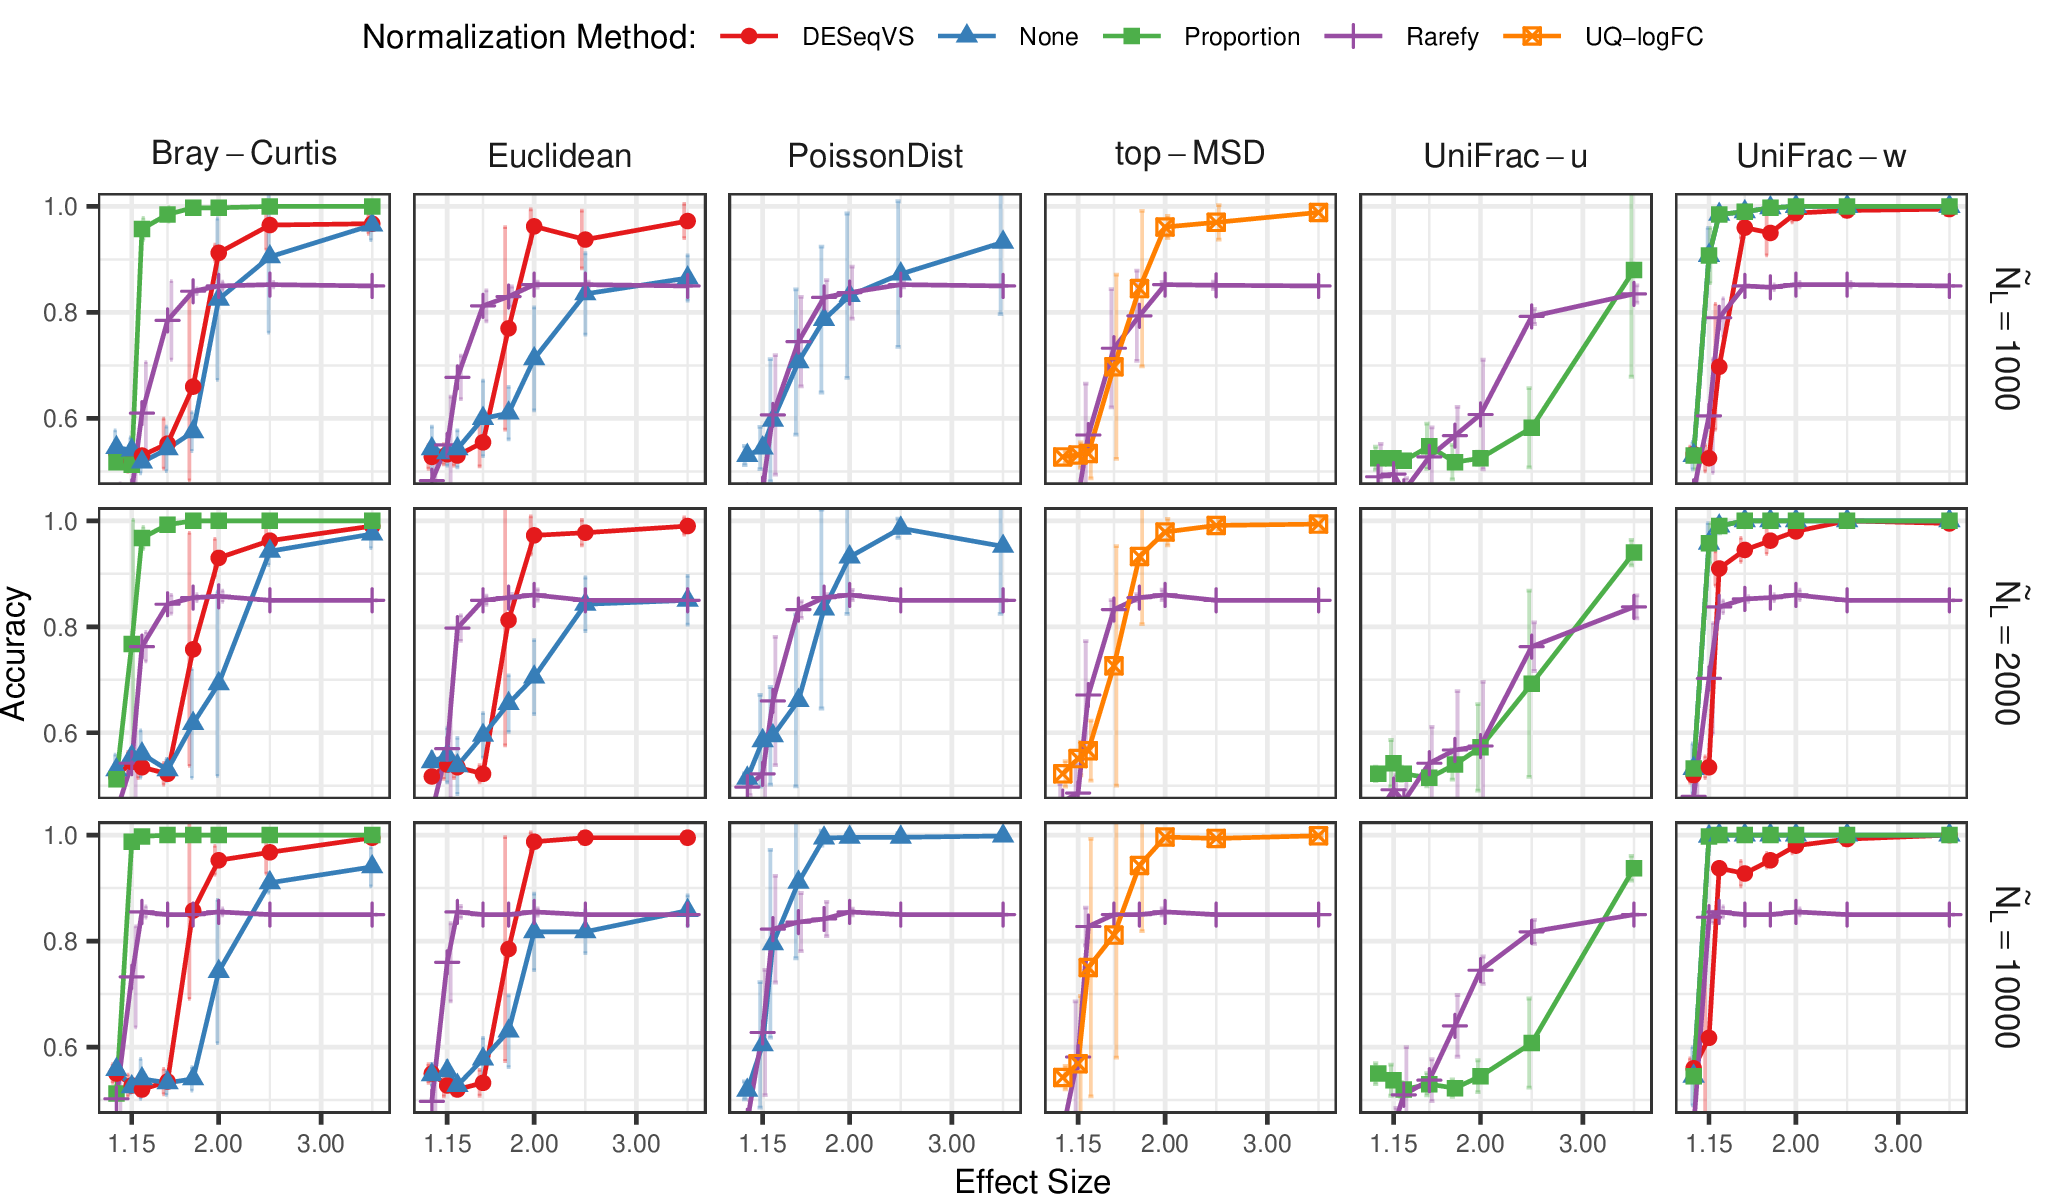
\includegraphics{figure_01.png}

\textbf{Figure 1. Re-running the R markdown provided in Protocol S1 of
WNWN qualitatively reproduced Figure 4 from WNWN.}

\newpage

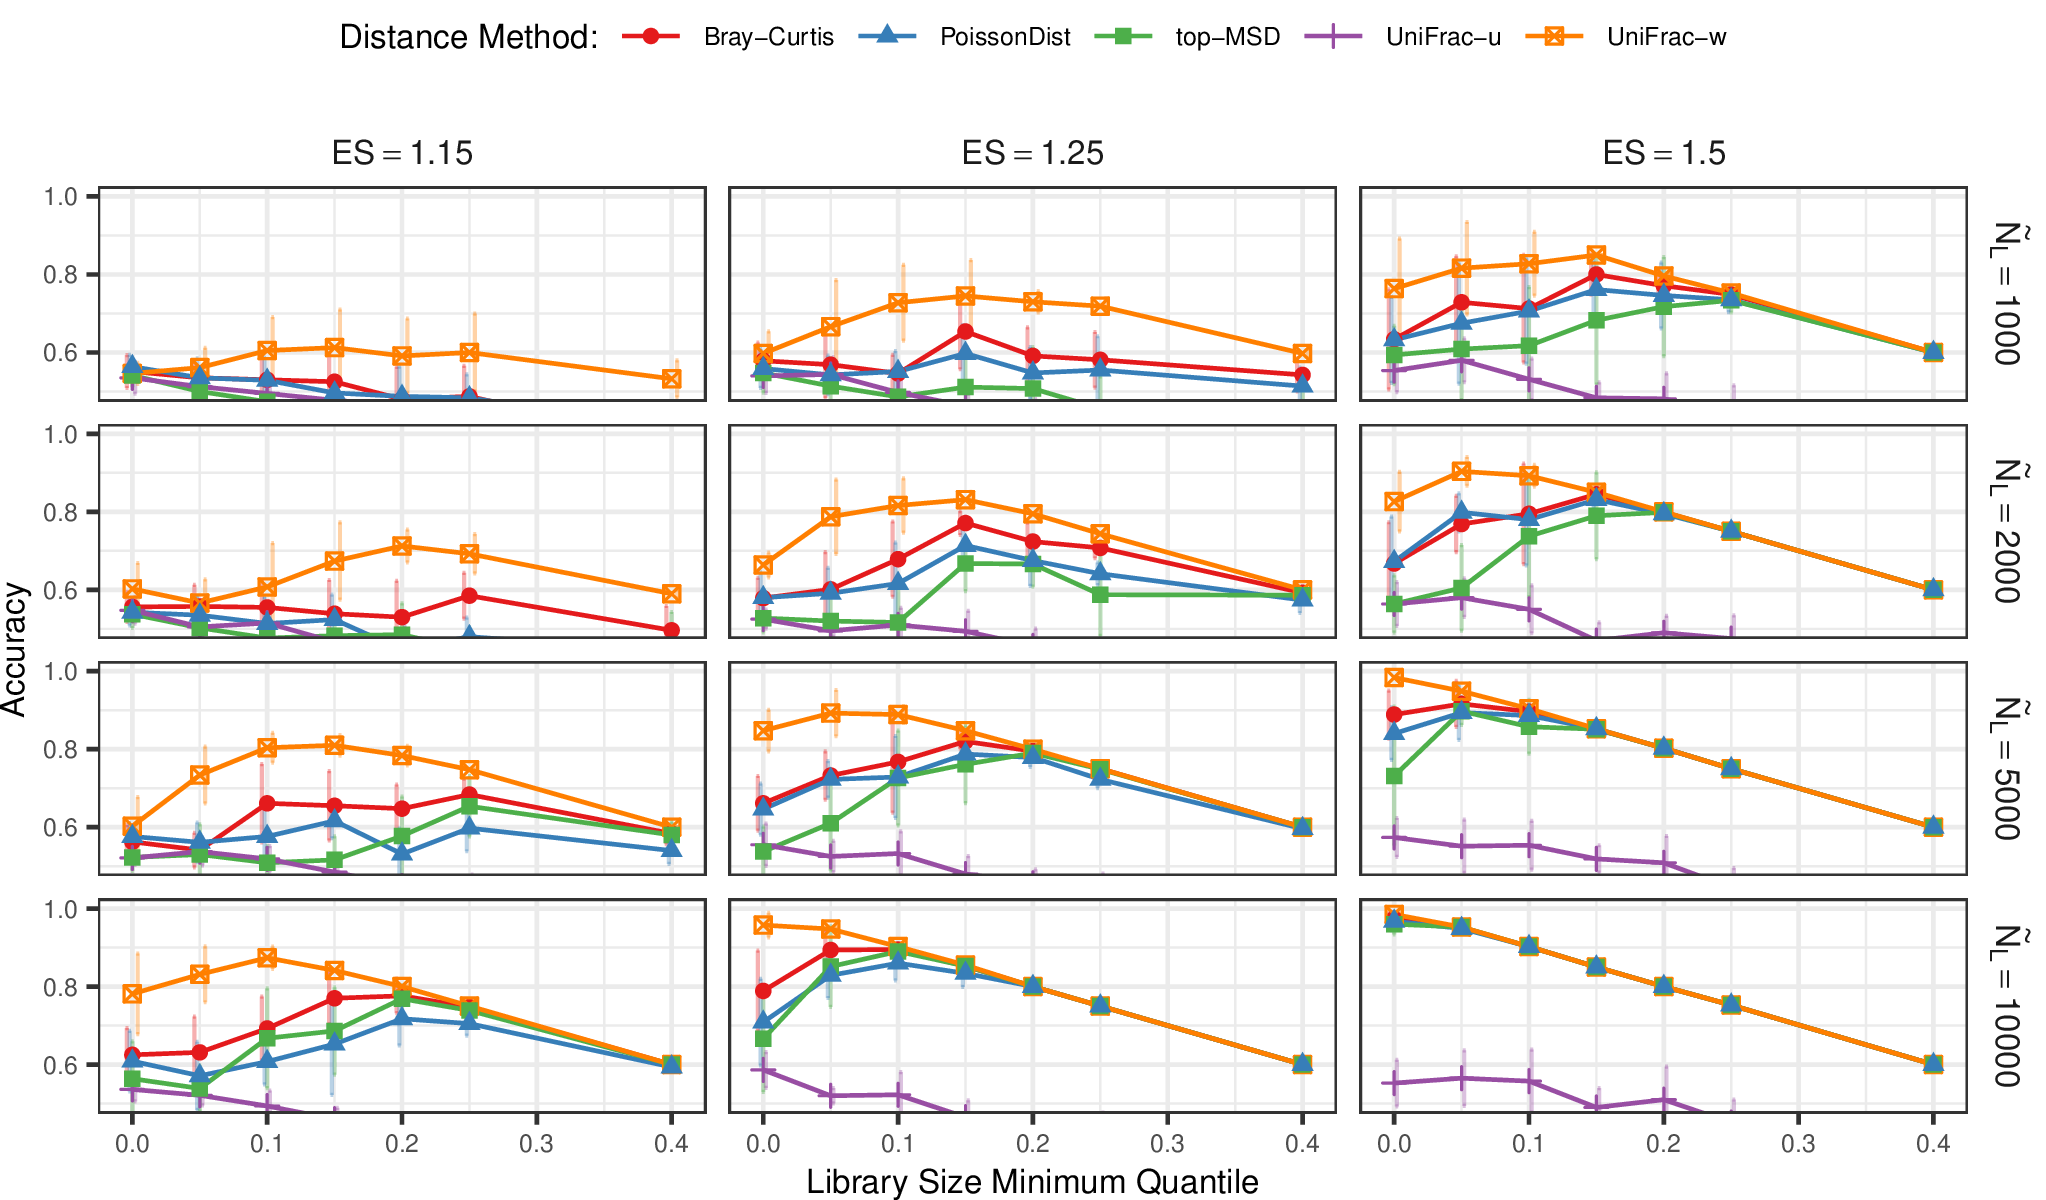
\includegraphics{figure_02.png}

\textbf{Figure 2. Re-running the R markdown provided in Protocol S1 of
WNWN qualitatively reproduced Figure 5 from WNWN.}

\newpage

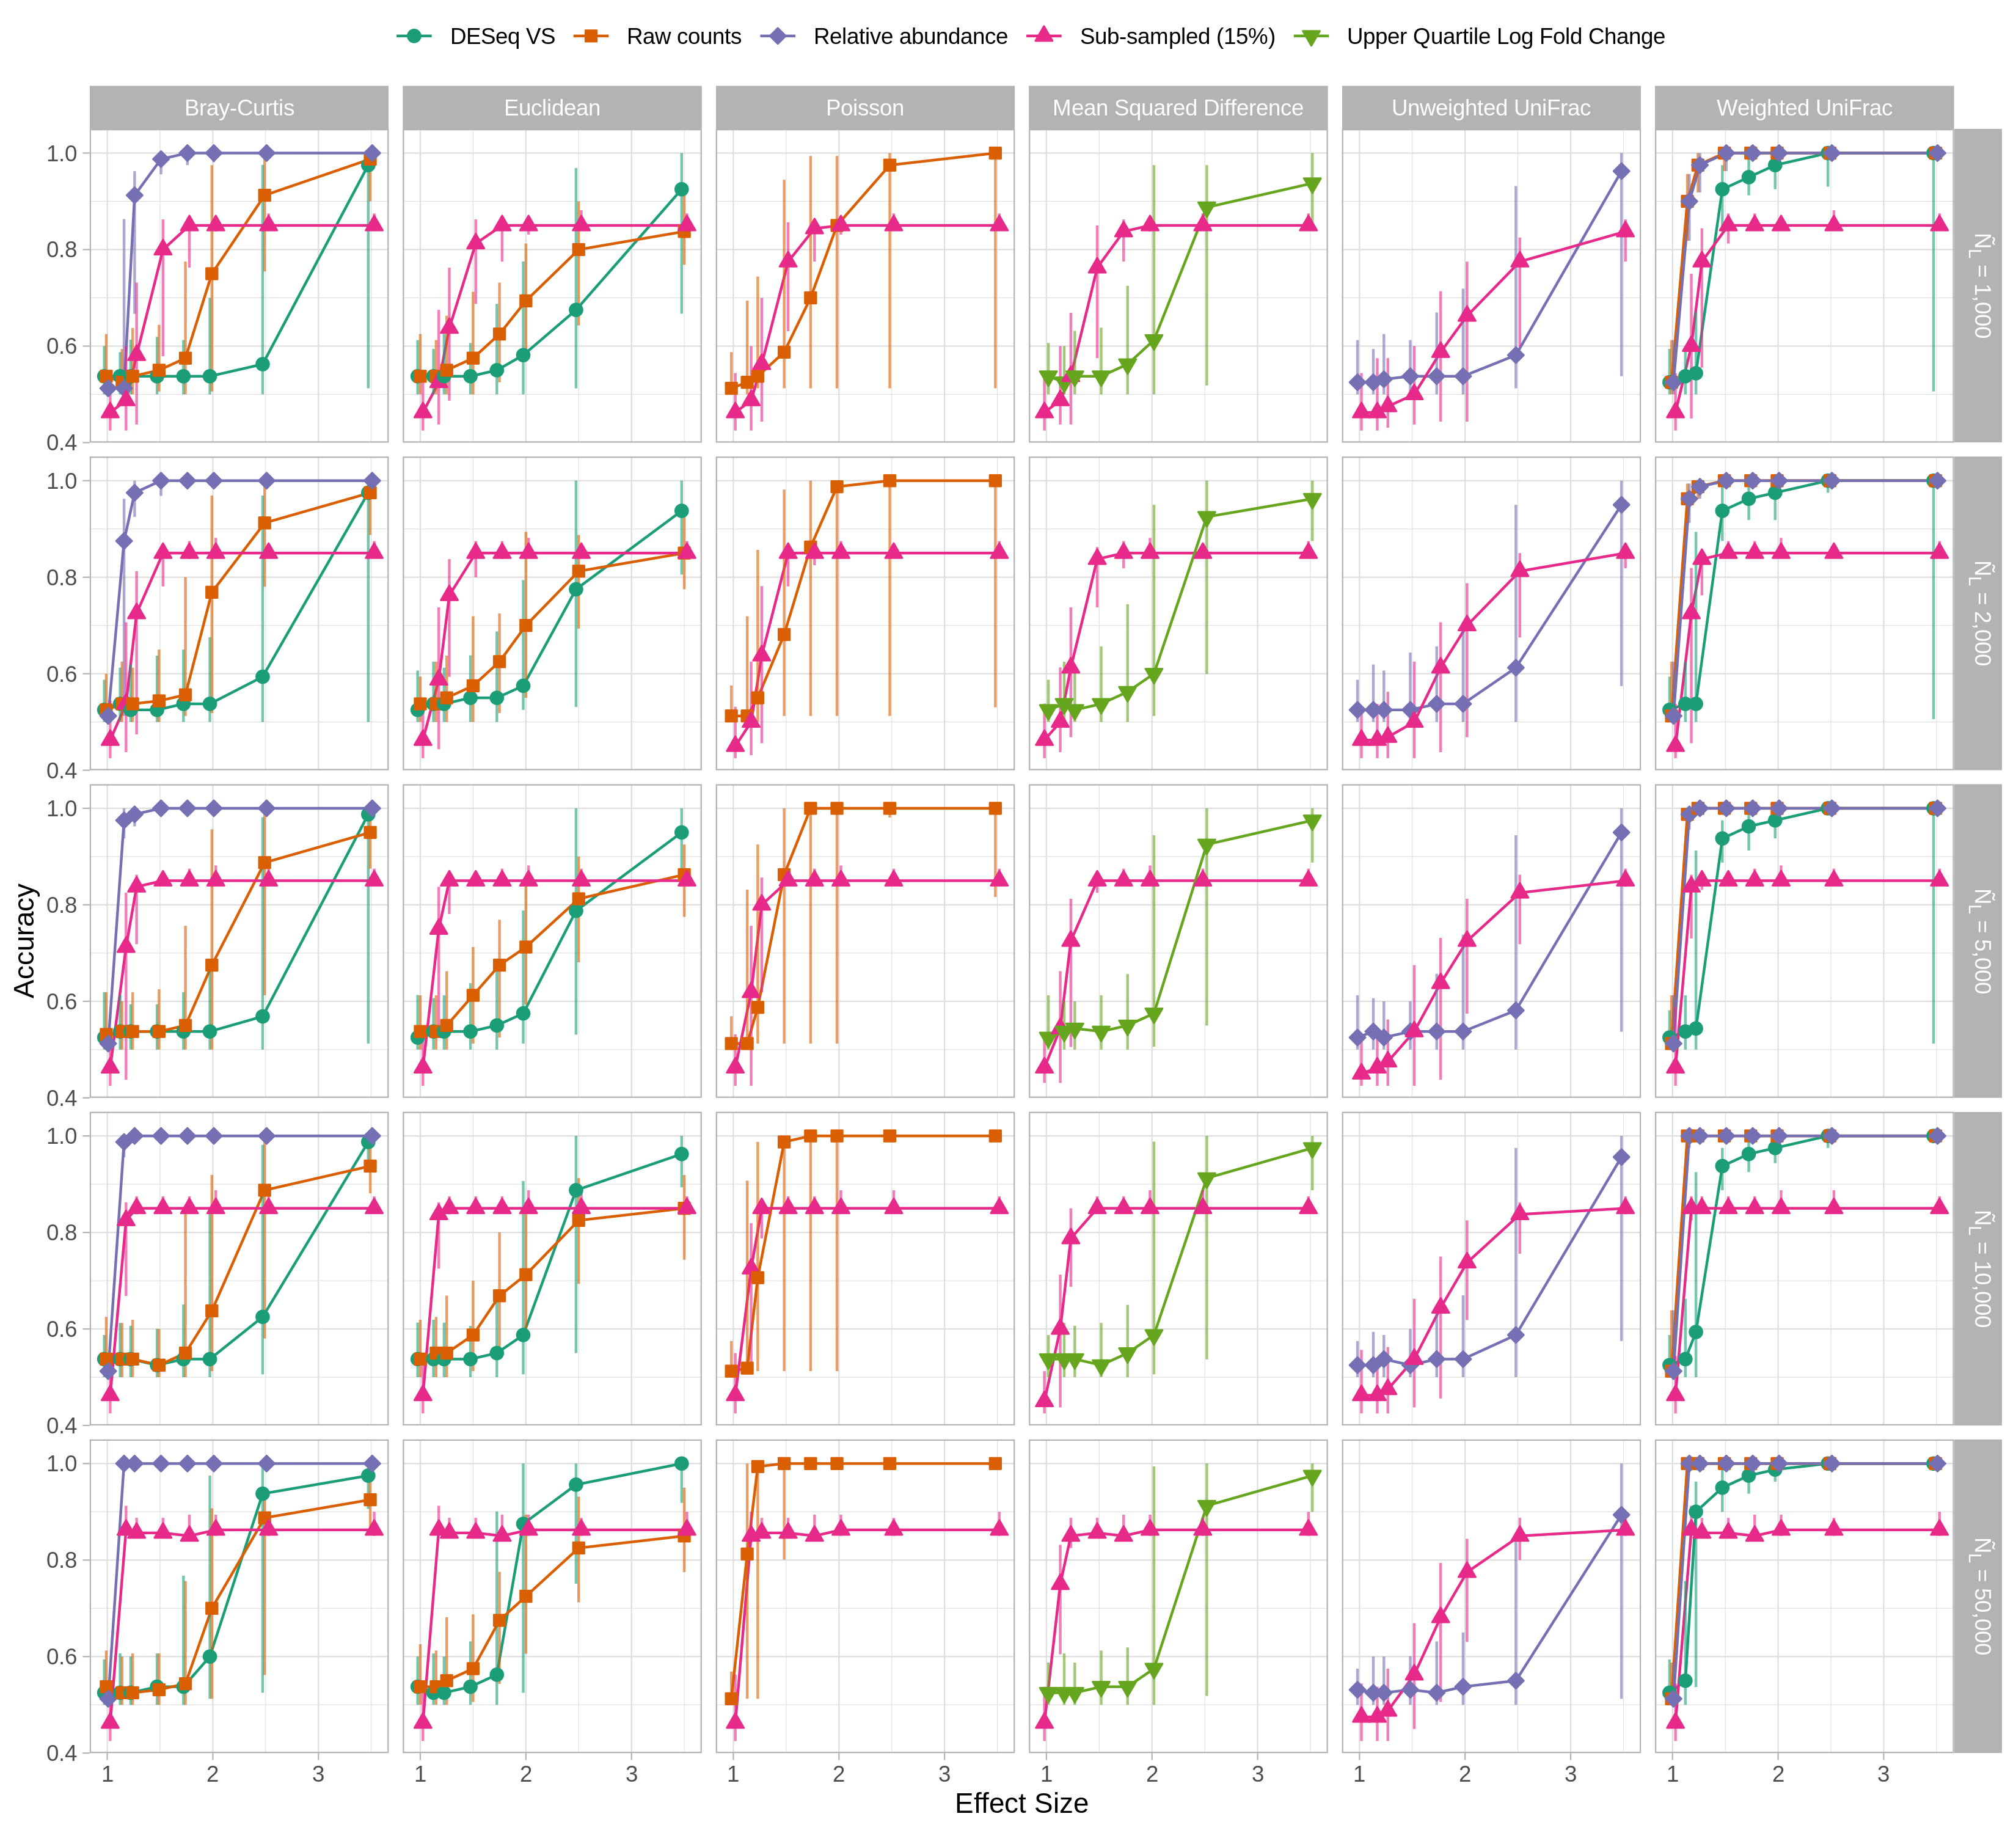
\includegraphics{figure_03.png}

\textbf{Figure 3. Successful reimplementation and expansion of analysis
presented in Figure 4 from WNWN in a Snakemake pipeline.} The
reimplemented workflow largely borrowed from the original
\texttt{simulation-cluster-accuracy-server.Rmd} R markdown file provided
in WNWN's Protocol S1. The most notable differences include the use of
100 rather than 5 randomizations and the addition of the median
sequencing depth (Ñ\textsubscript{L}) of 50,000. The plotting symbols
indicate the median of 100 randomizations and the error bars represent
the observed 95\% confidence interval. Simulations run at the same
effect size are dodged to better reveal overlapping data. The sequencing
depths were drawn from the GlobalPatterns dataset and sequences were
clustered using PAM.

\newpage

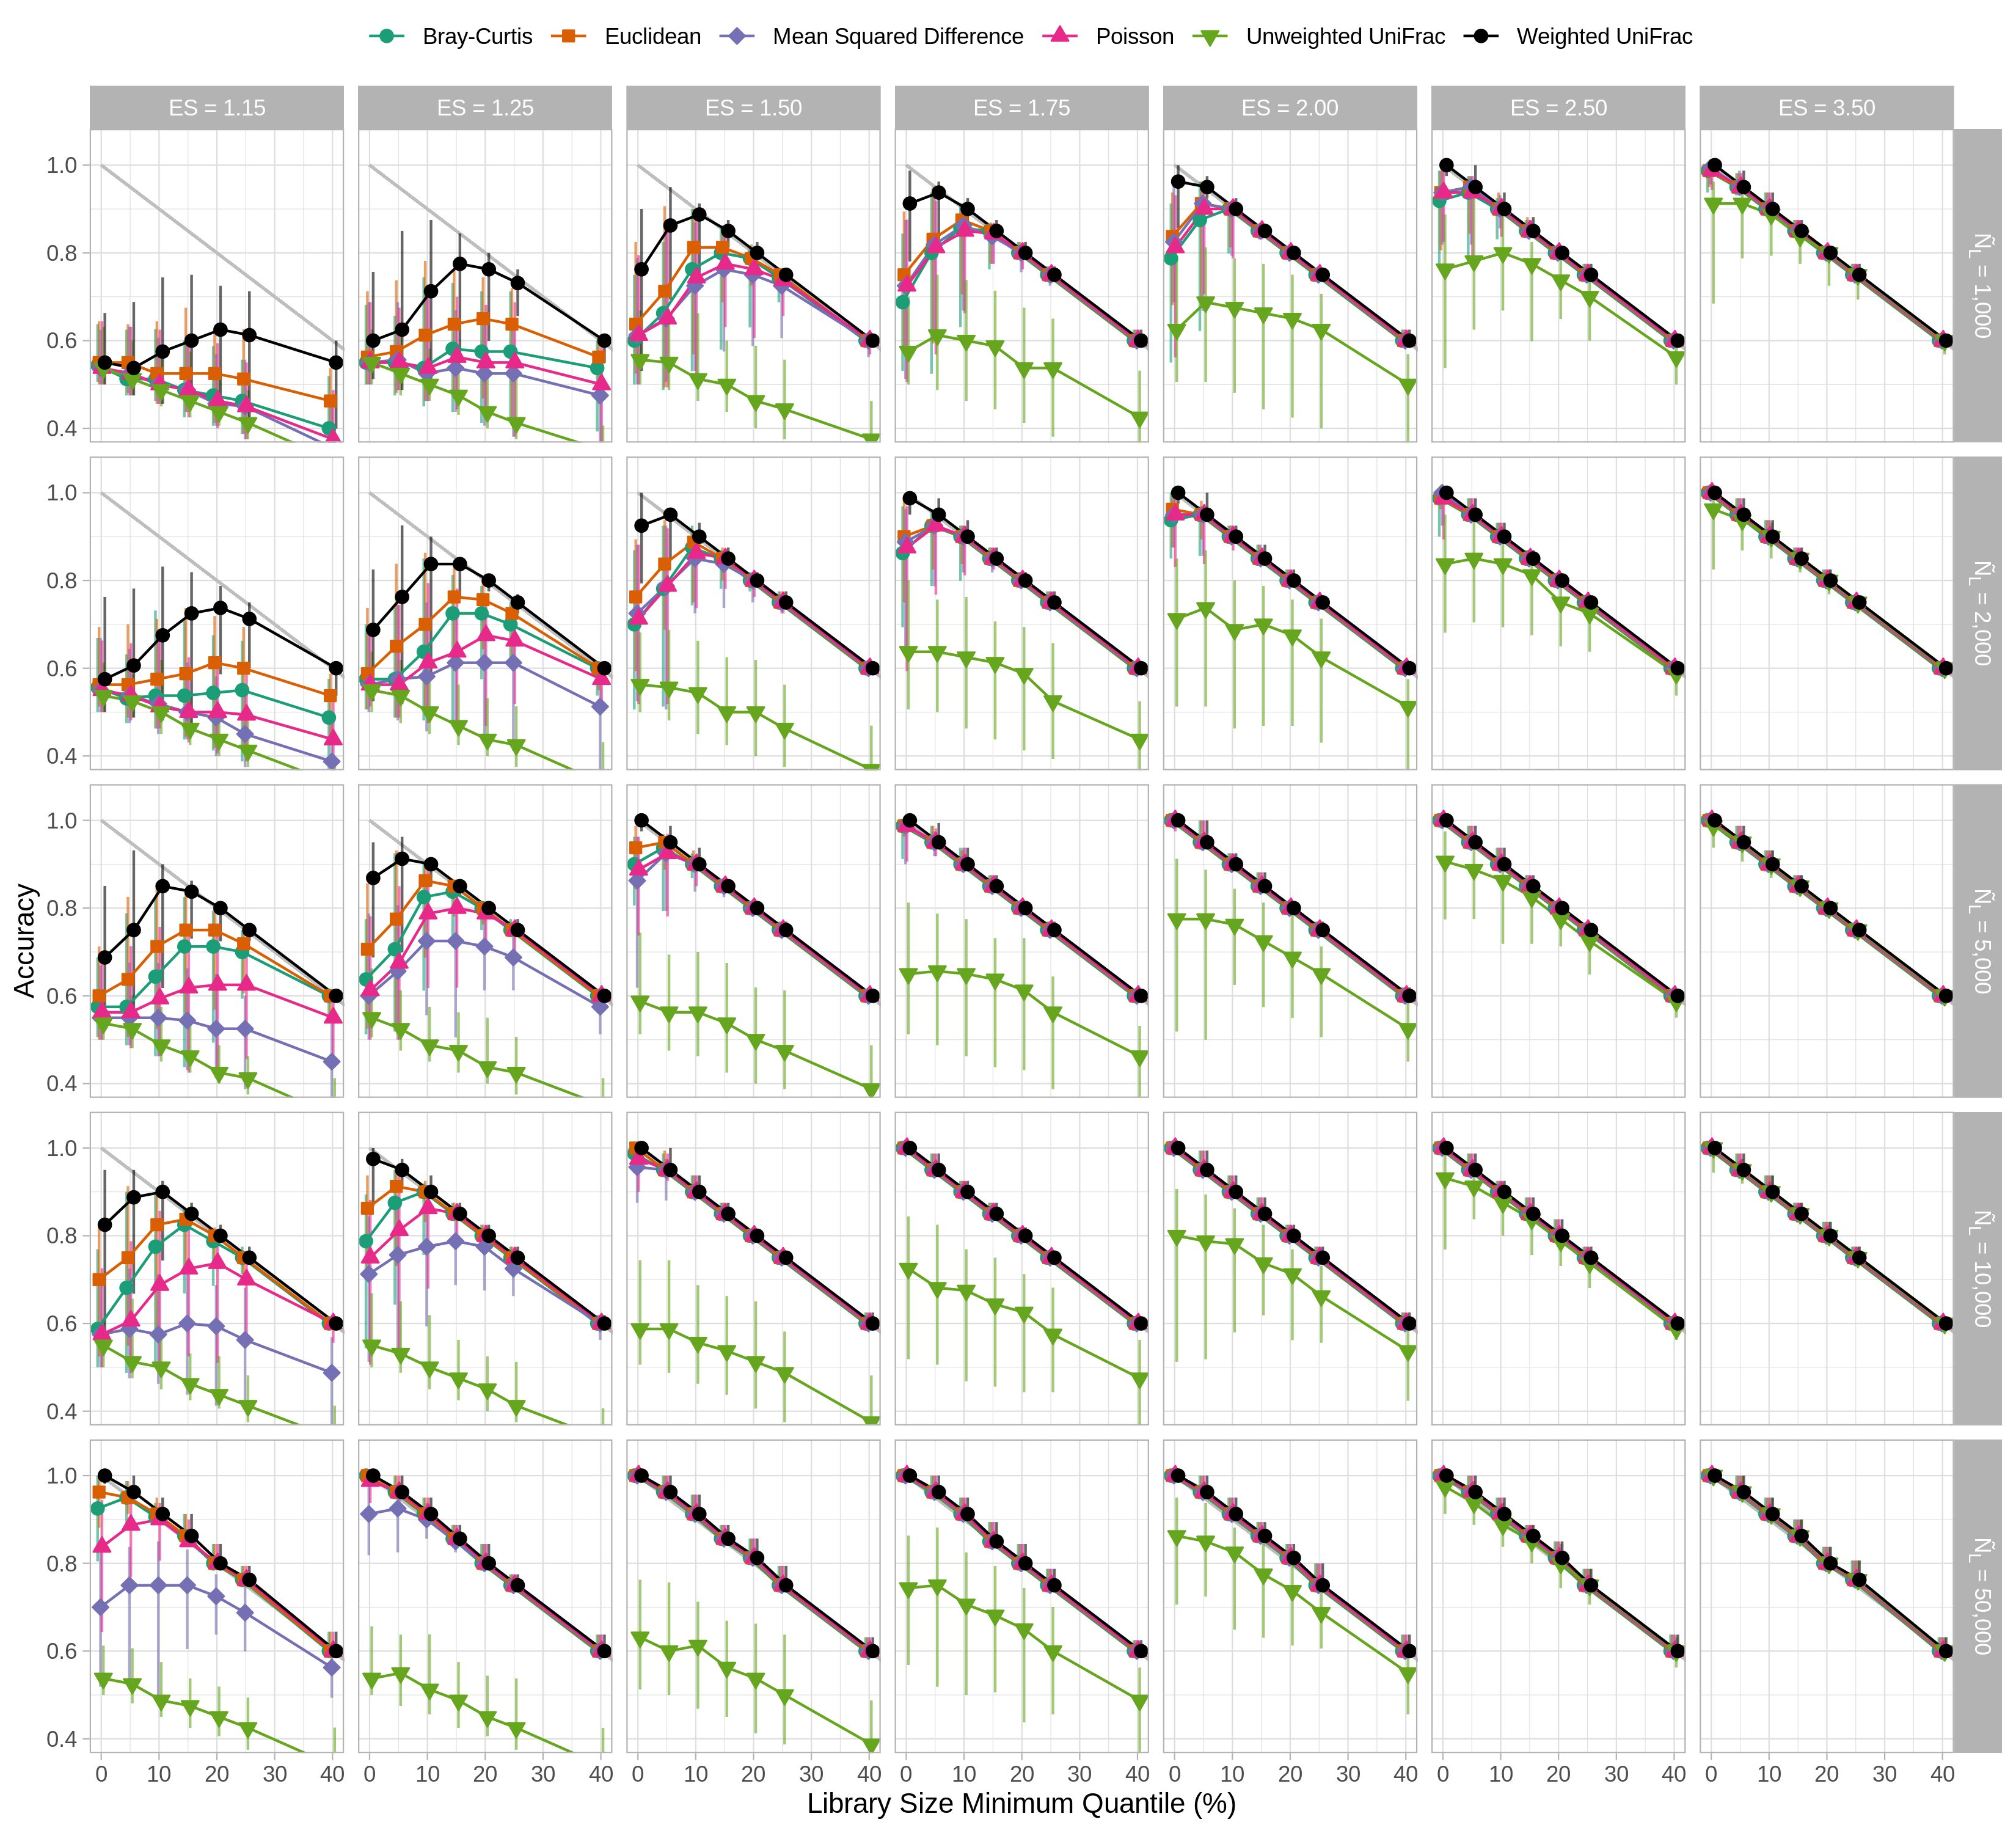
\includegraphics{figure_04.png}

\textbf{Figure 4. Successful reimplementation and expansion of analysis
presented in Figure 5 from WNWN in a Snakemake pipeline.} The
reimplemented workflow largely borrowed from the original
\texttt{simulation-cluster-accuracy-server.Rmd} R markdown file provided
in WNWN's Protocol S1. The most notable differences include the use of
100 rather than 5 randomizations and the addition of the median
sequencing depth (Ñ\textsubscript{L}) of 50,000. The plotting symbols
indicate the median of 100 randomizations and the error bars represent
the observed 95\% confidence interval. Simulations run at the same
effect size are dodged to better reveal overlapping data. A light gray
line is shown to indicate the best possible accuracy for each library
size minimum quantile value. The sequencing depths were drawn from the
GlobalPatterns dataset and sequences were clustered using PAM.

\newpage

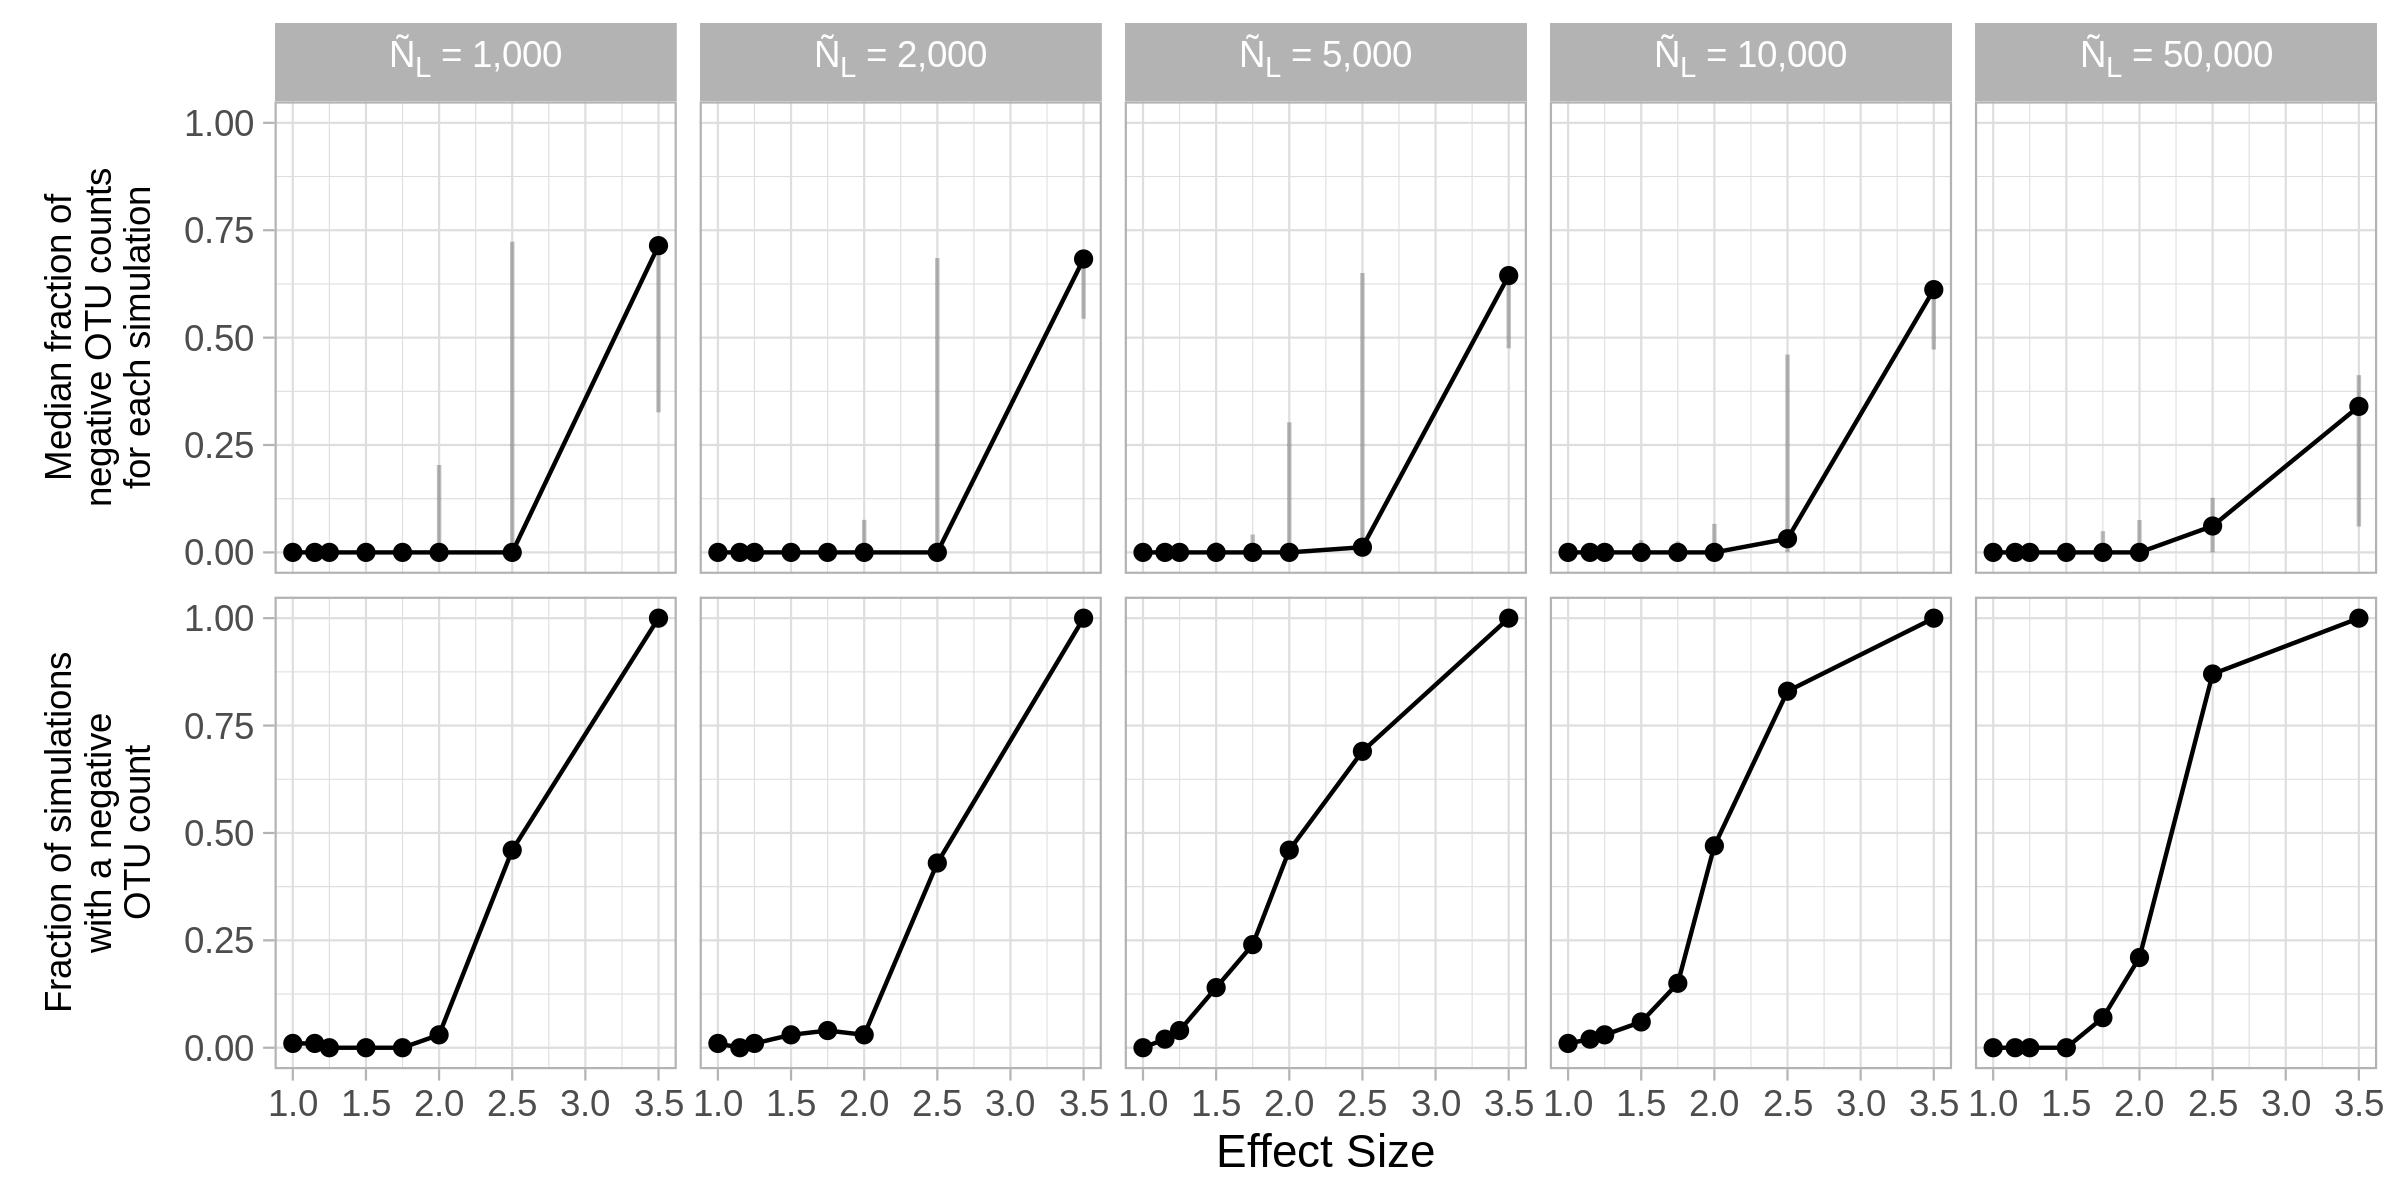
\includegraphics{figure_05.png}

\textbf{Figure 5. DESeq Variance Stabilization of OTU counts resulted in
negative values that were used to calculate Bray-Curtis and Weighted
UniFrac distances.} The median number of negative OTU counts that had a
negative OTU count following normalization increased with the effect
size and decreased as Ñ\textsubscript{L} increased (first row). The
error bars indicate the observe 95\% confidence interval. The fraction
simulated datasets that had a negative OTU count following normalization
also increased with effect size, but increased as Ñ\textsubscript{L}
increased (second row). For each effect size there were 100 replicate
datasets.

\newpage

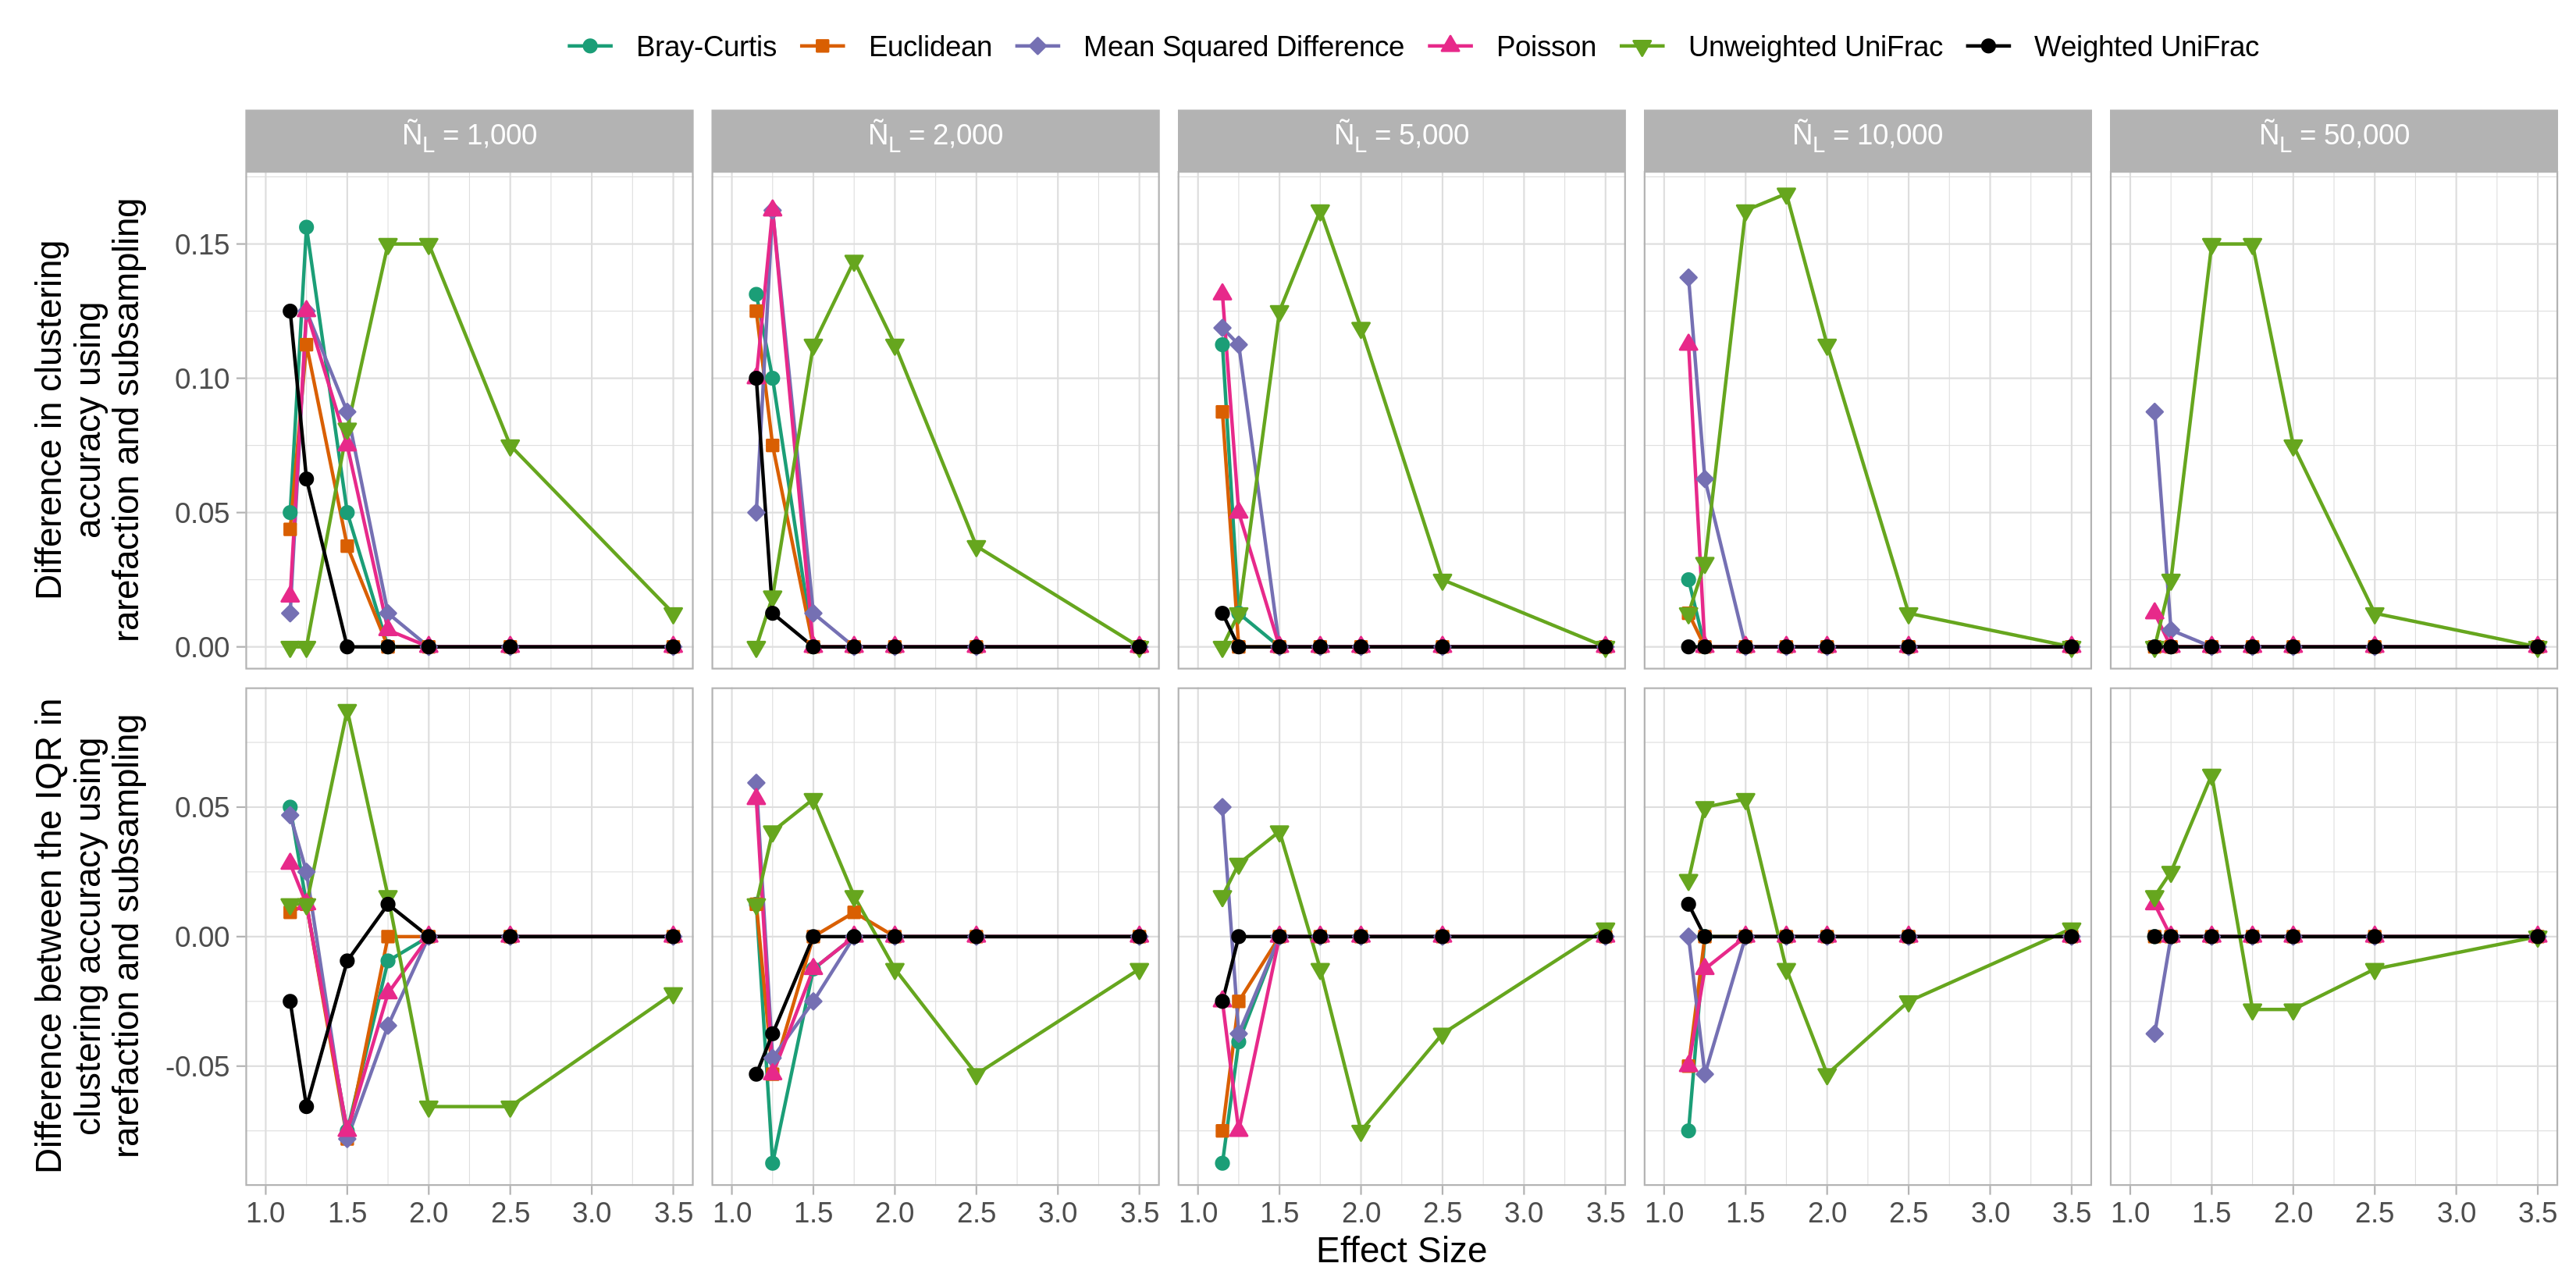
\includegraphics{figure_06.png}

\textbf{Figure 6. Rarefaction resulted in larger and less variable
clustering accuracies.} With the exception of Unweighted UniFrac
distances, the improved performance by rarefaction was observed at
smaller effect sizes. In the first row of panels larger values mean that
the accuracies by rarefaction were better than those of subsampling. In
the second row of samples, larger values mean that interquartile range
(IQR) for rarefaction was larger than that of subsampling.

\newpage

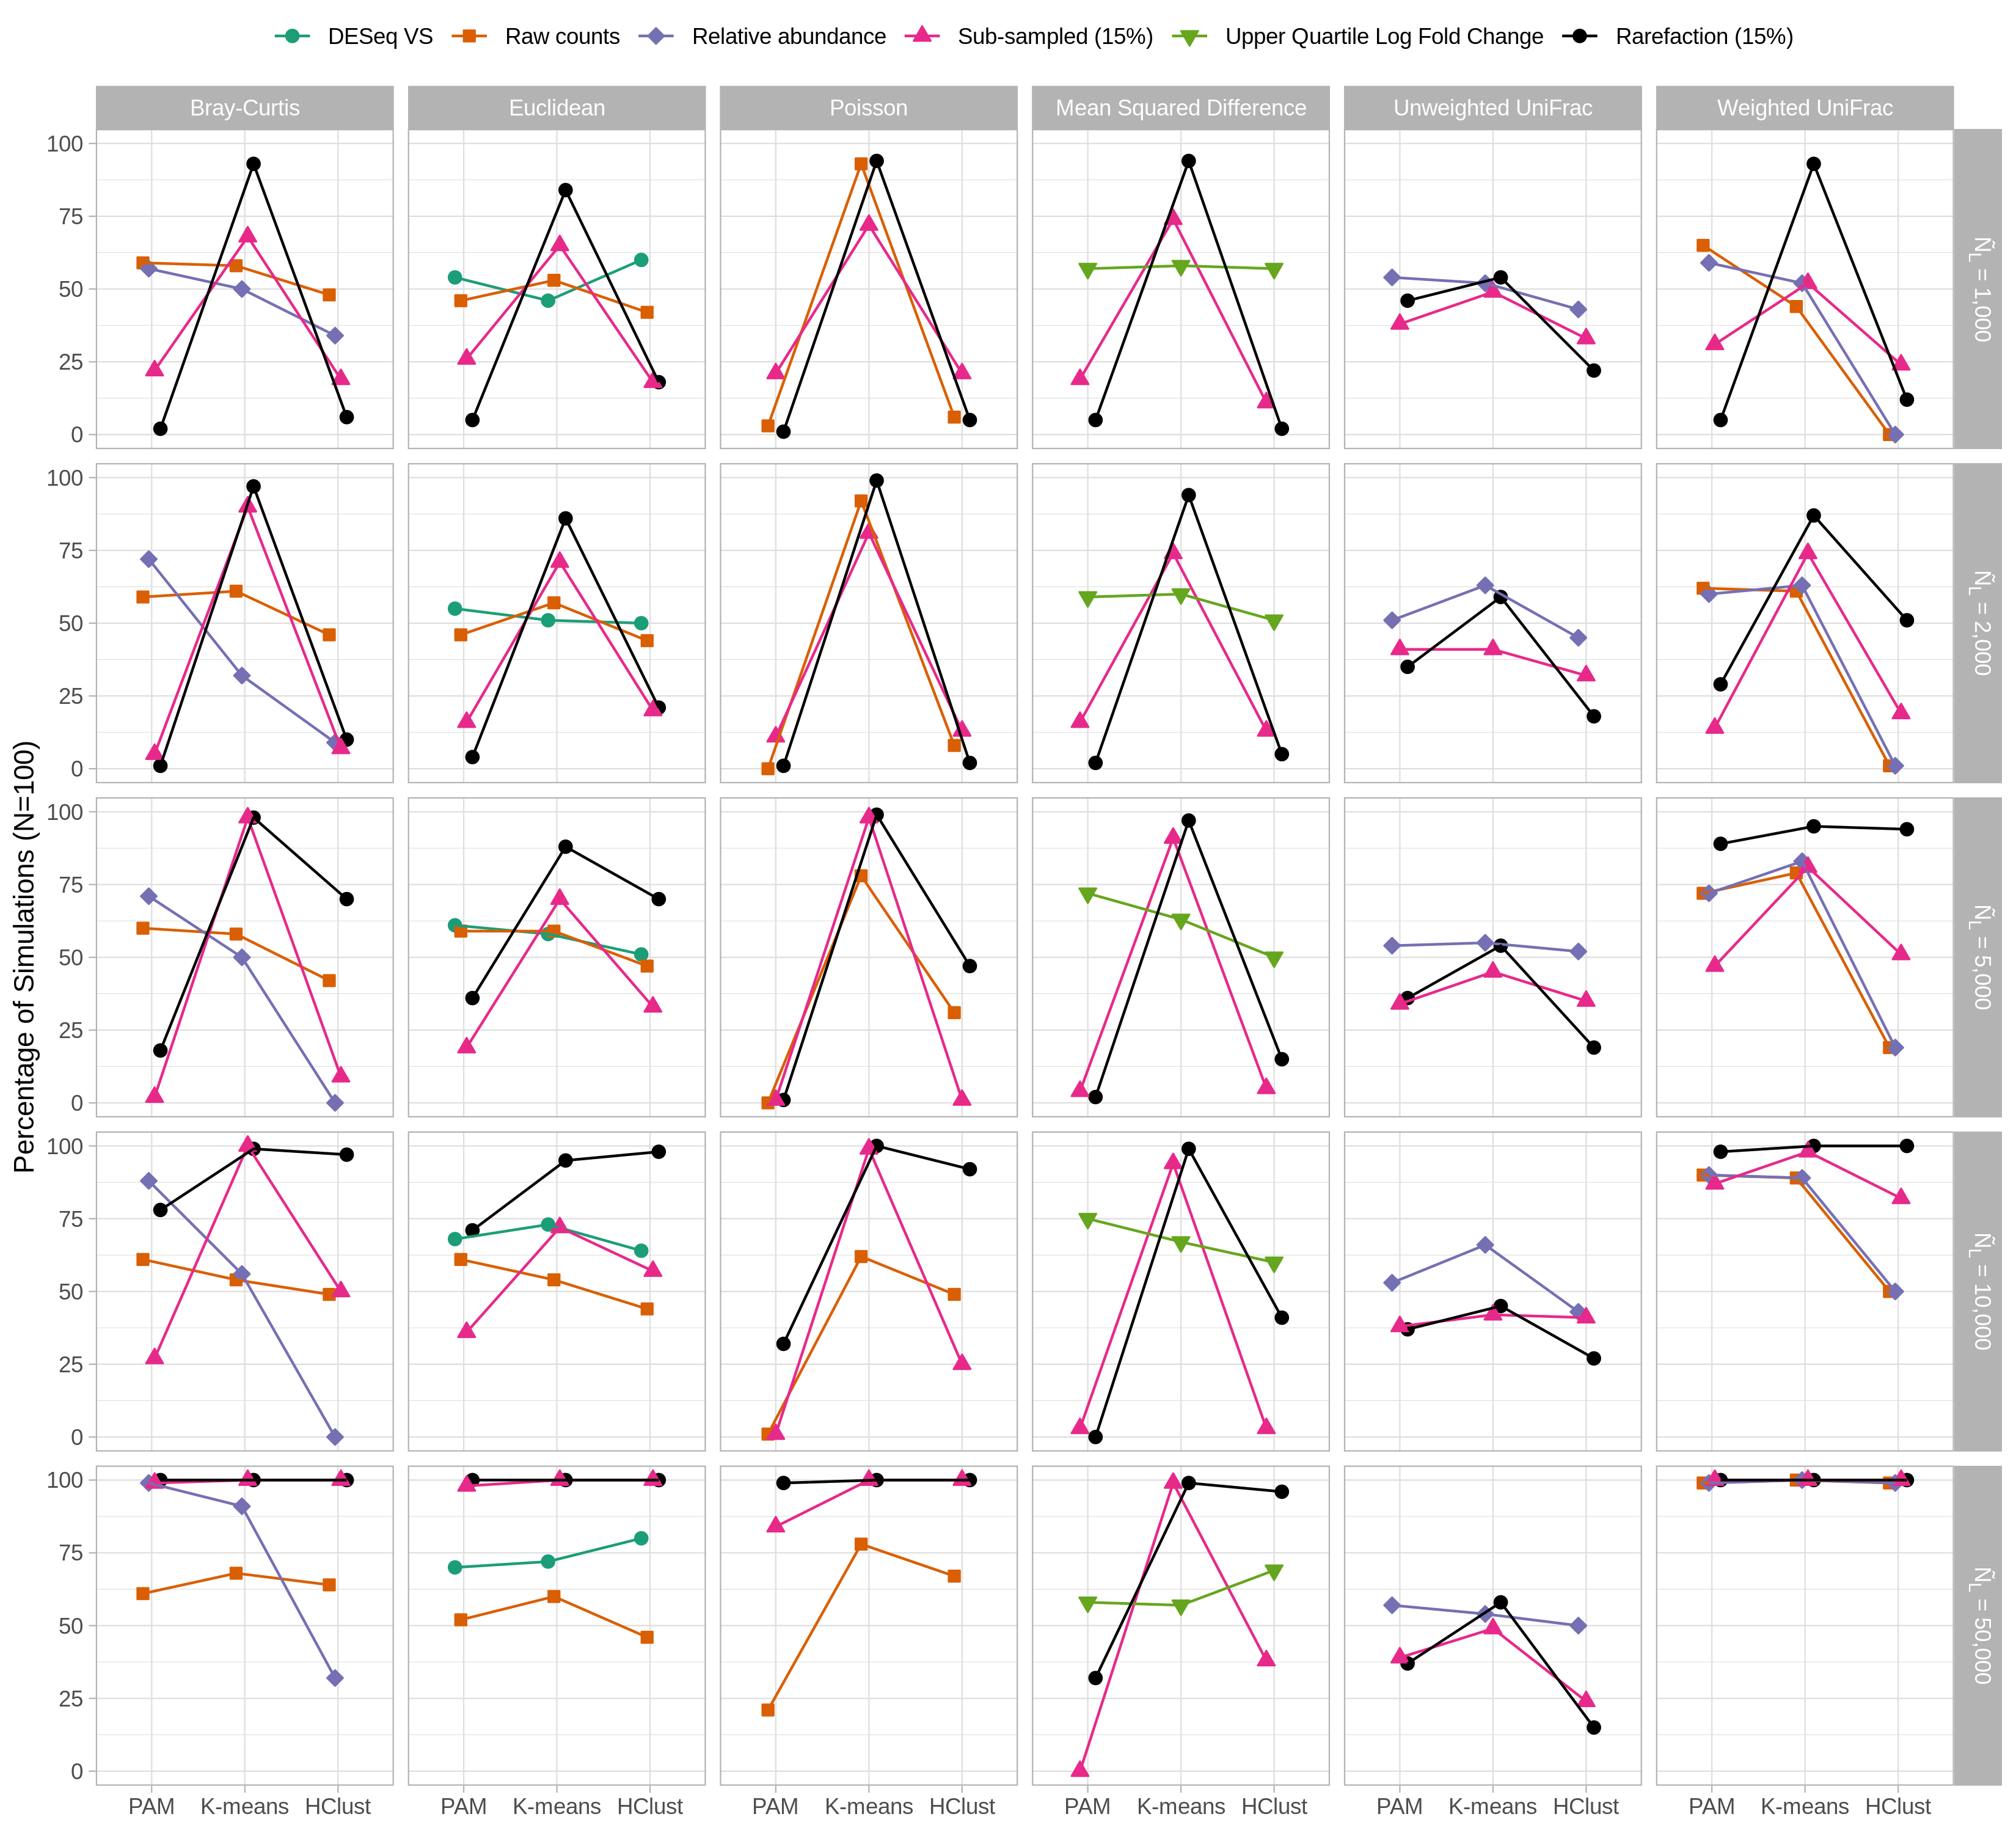
\includegraphics{figure_07.png}

\textbf{Figure 7. K-means clustering was consistently as good or better
than PAM or hierarchical clustering when comparing rarefaction to other
normalization methods.} Each point represents the percentage of 100
simulations where that clustering method performed as well or better
than the other methods for that normalization procedure.

\newpage

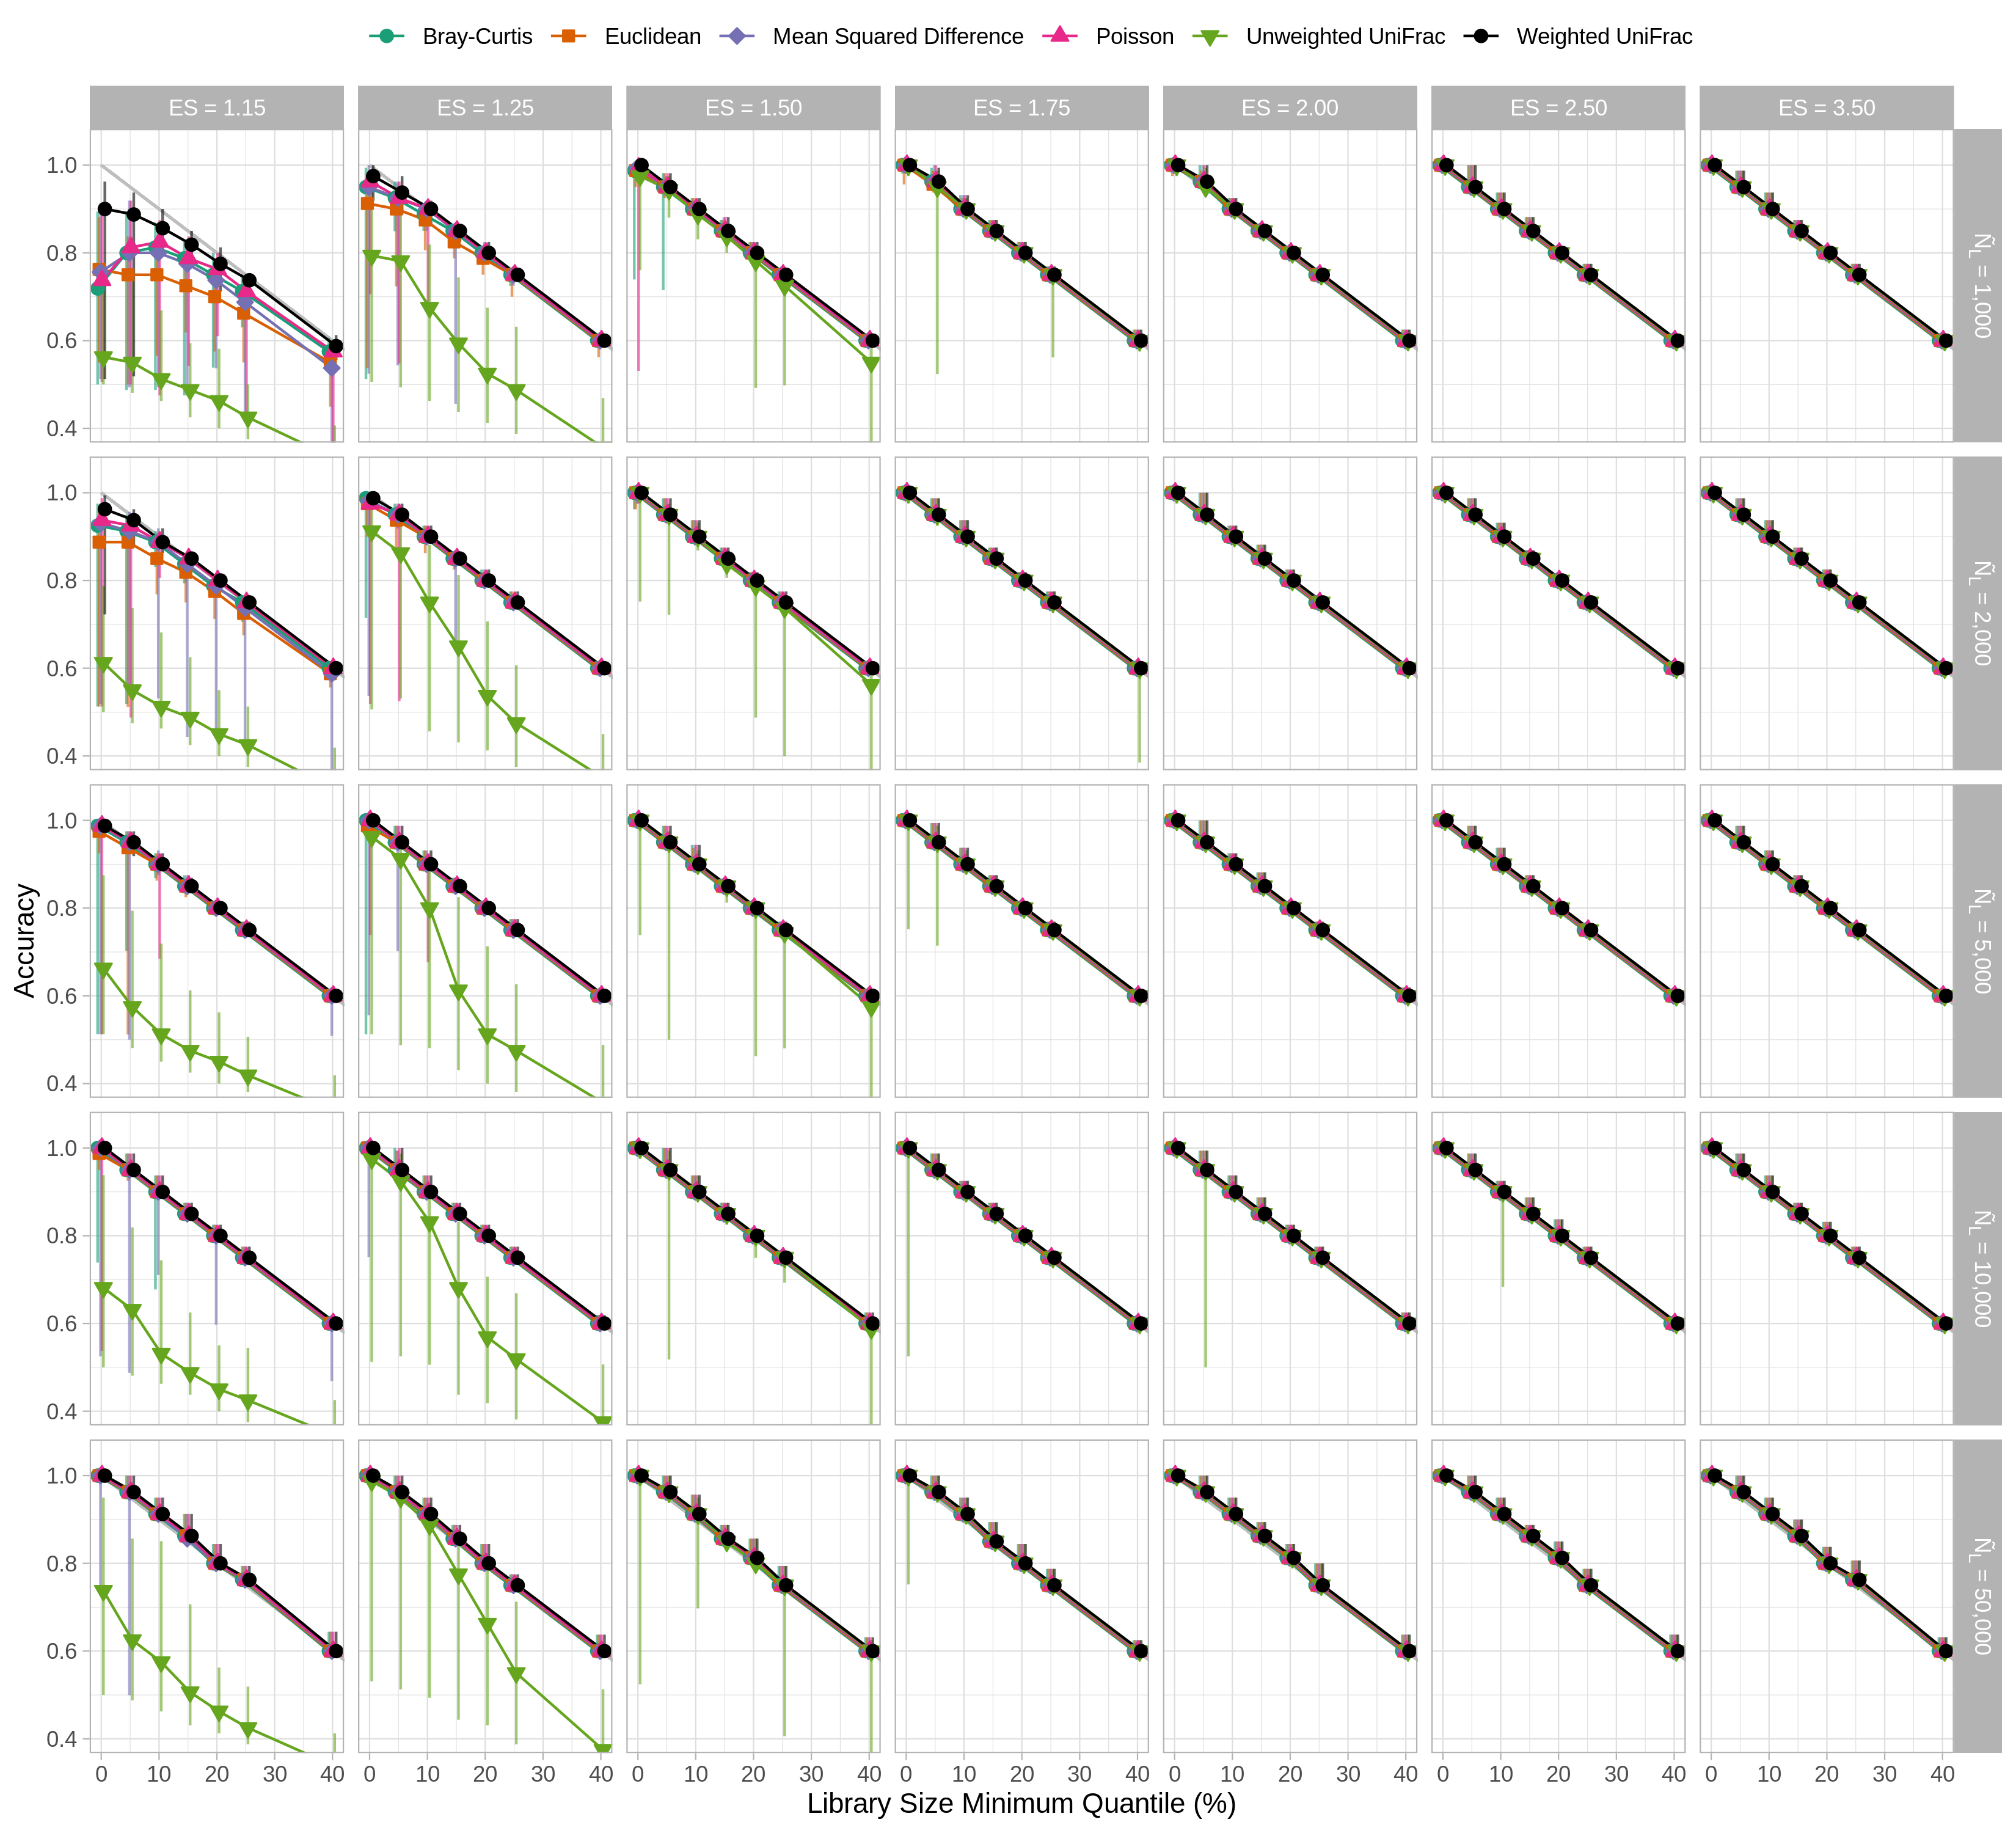
\includegraphics{figure_08.png}

\textbf{Figure 8. When the median sequencing depth was 2,000 sequences
or more, rarefaction of the entire dataset performed better than
removing the smallest 15\% of samples when using K-means clustering.}
This figure is analogous to Figure 4 except that K-means clustering was
used instead of PAM.

\newpage

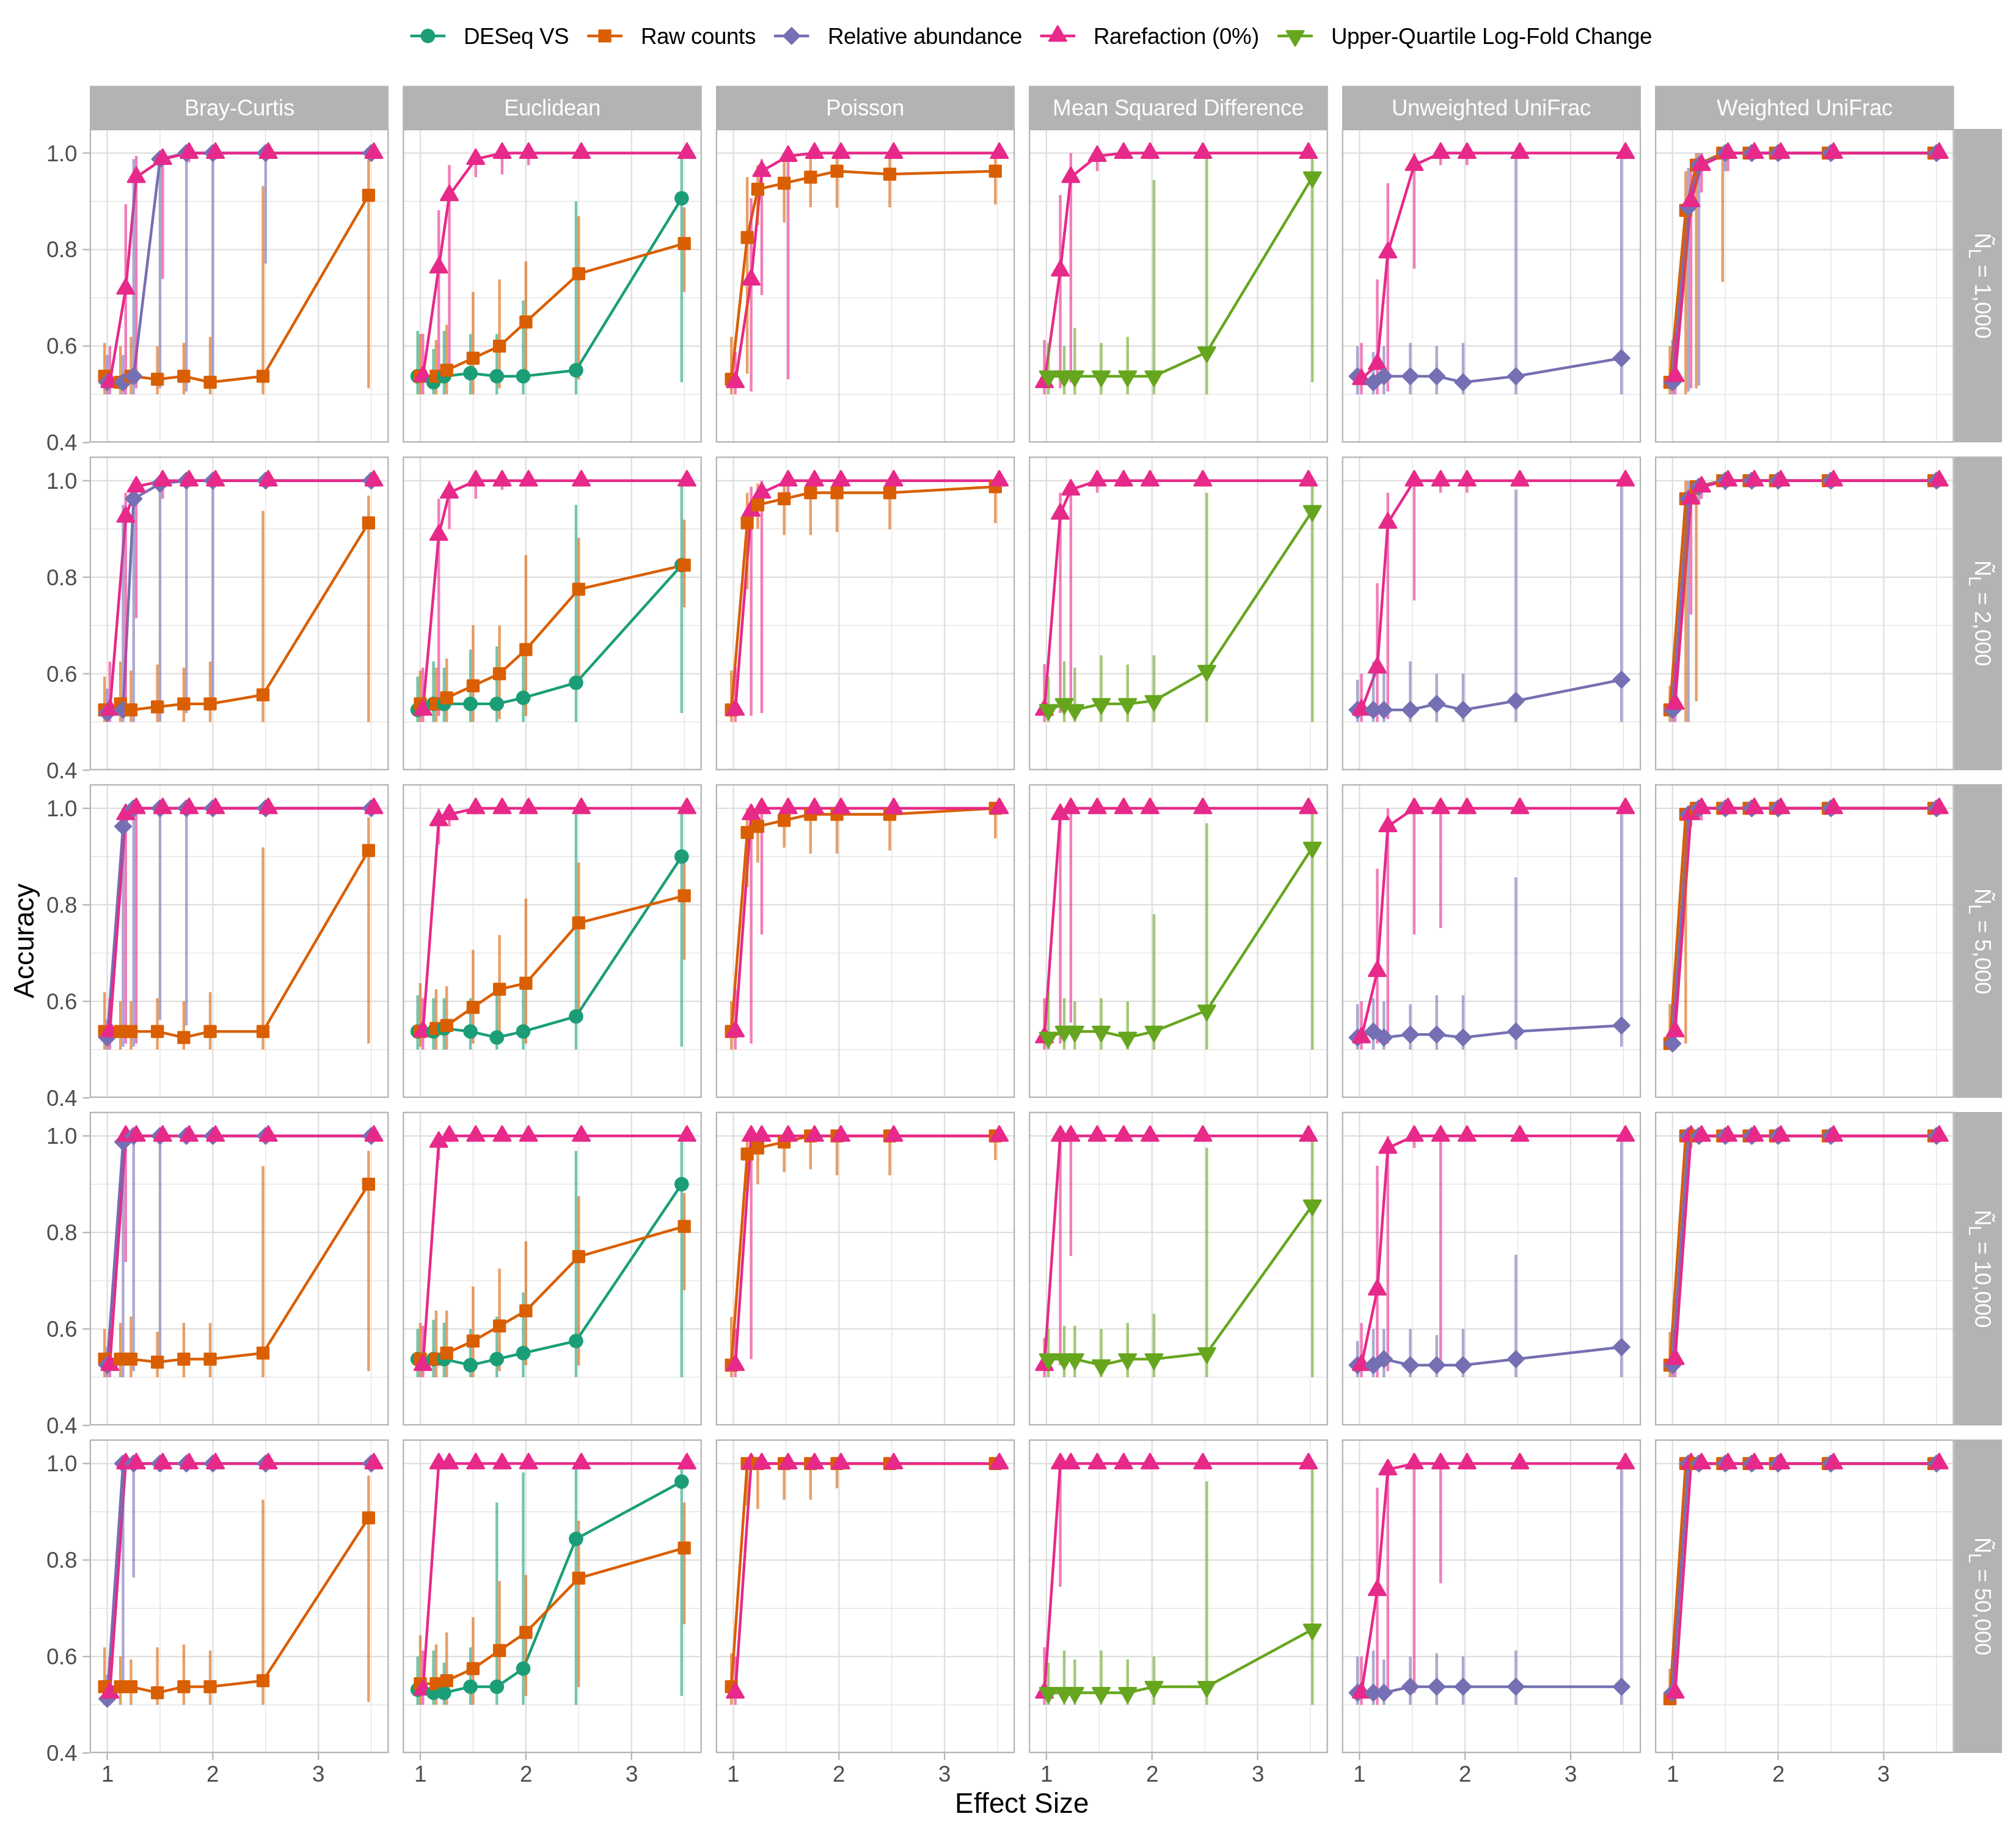
\includegraphics{figure_09.png}

\textbf{Figure 9. K-means clustering of distances calculated with
rarefaction were as good or better than any other normalization method.}
This figure is analogous to Figure 3 except that K-means clustering was
used instead of PAM, rarefaction on the full dataset was used instead of
subsampling to the size of the sample at the 15th percentile, and DESeq
Variance Stabilization normalized OTU counts were only used with
Euclidean distances.

\newpage

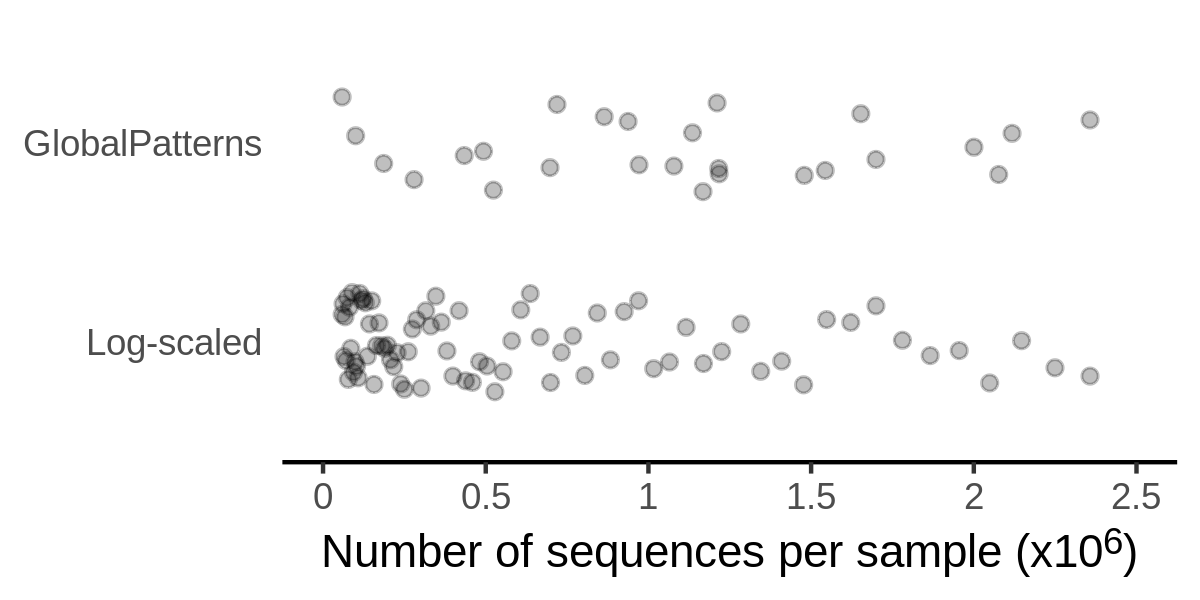
\includegraphics{figure_10.png}

\textbf{Figure 10. Comparison of the normally distributed sequencing
depths from the GlobalPatterns dataset and a log-scaled distribution of
sequencing depths.} The log-scaled distribution was generated so that
each sample in a simulation could have a unique number of sequences and
to simulate the skew right distribution commonly seen in microbiome
studies.

\newpage

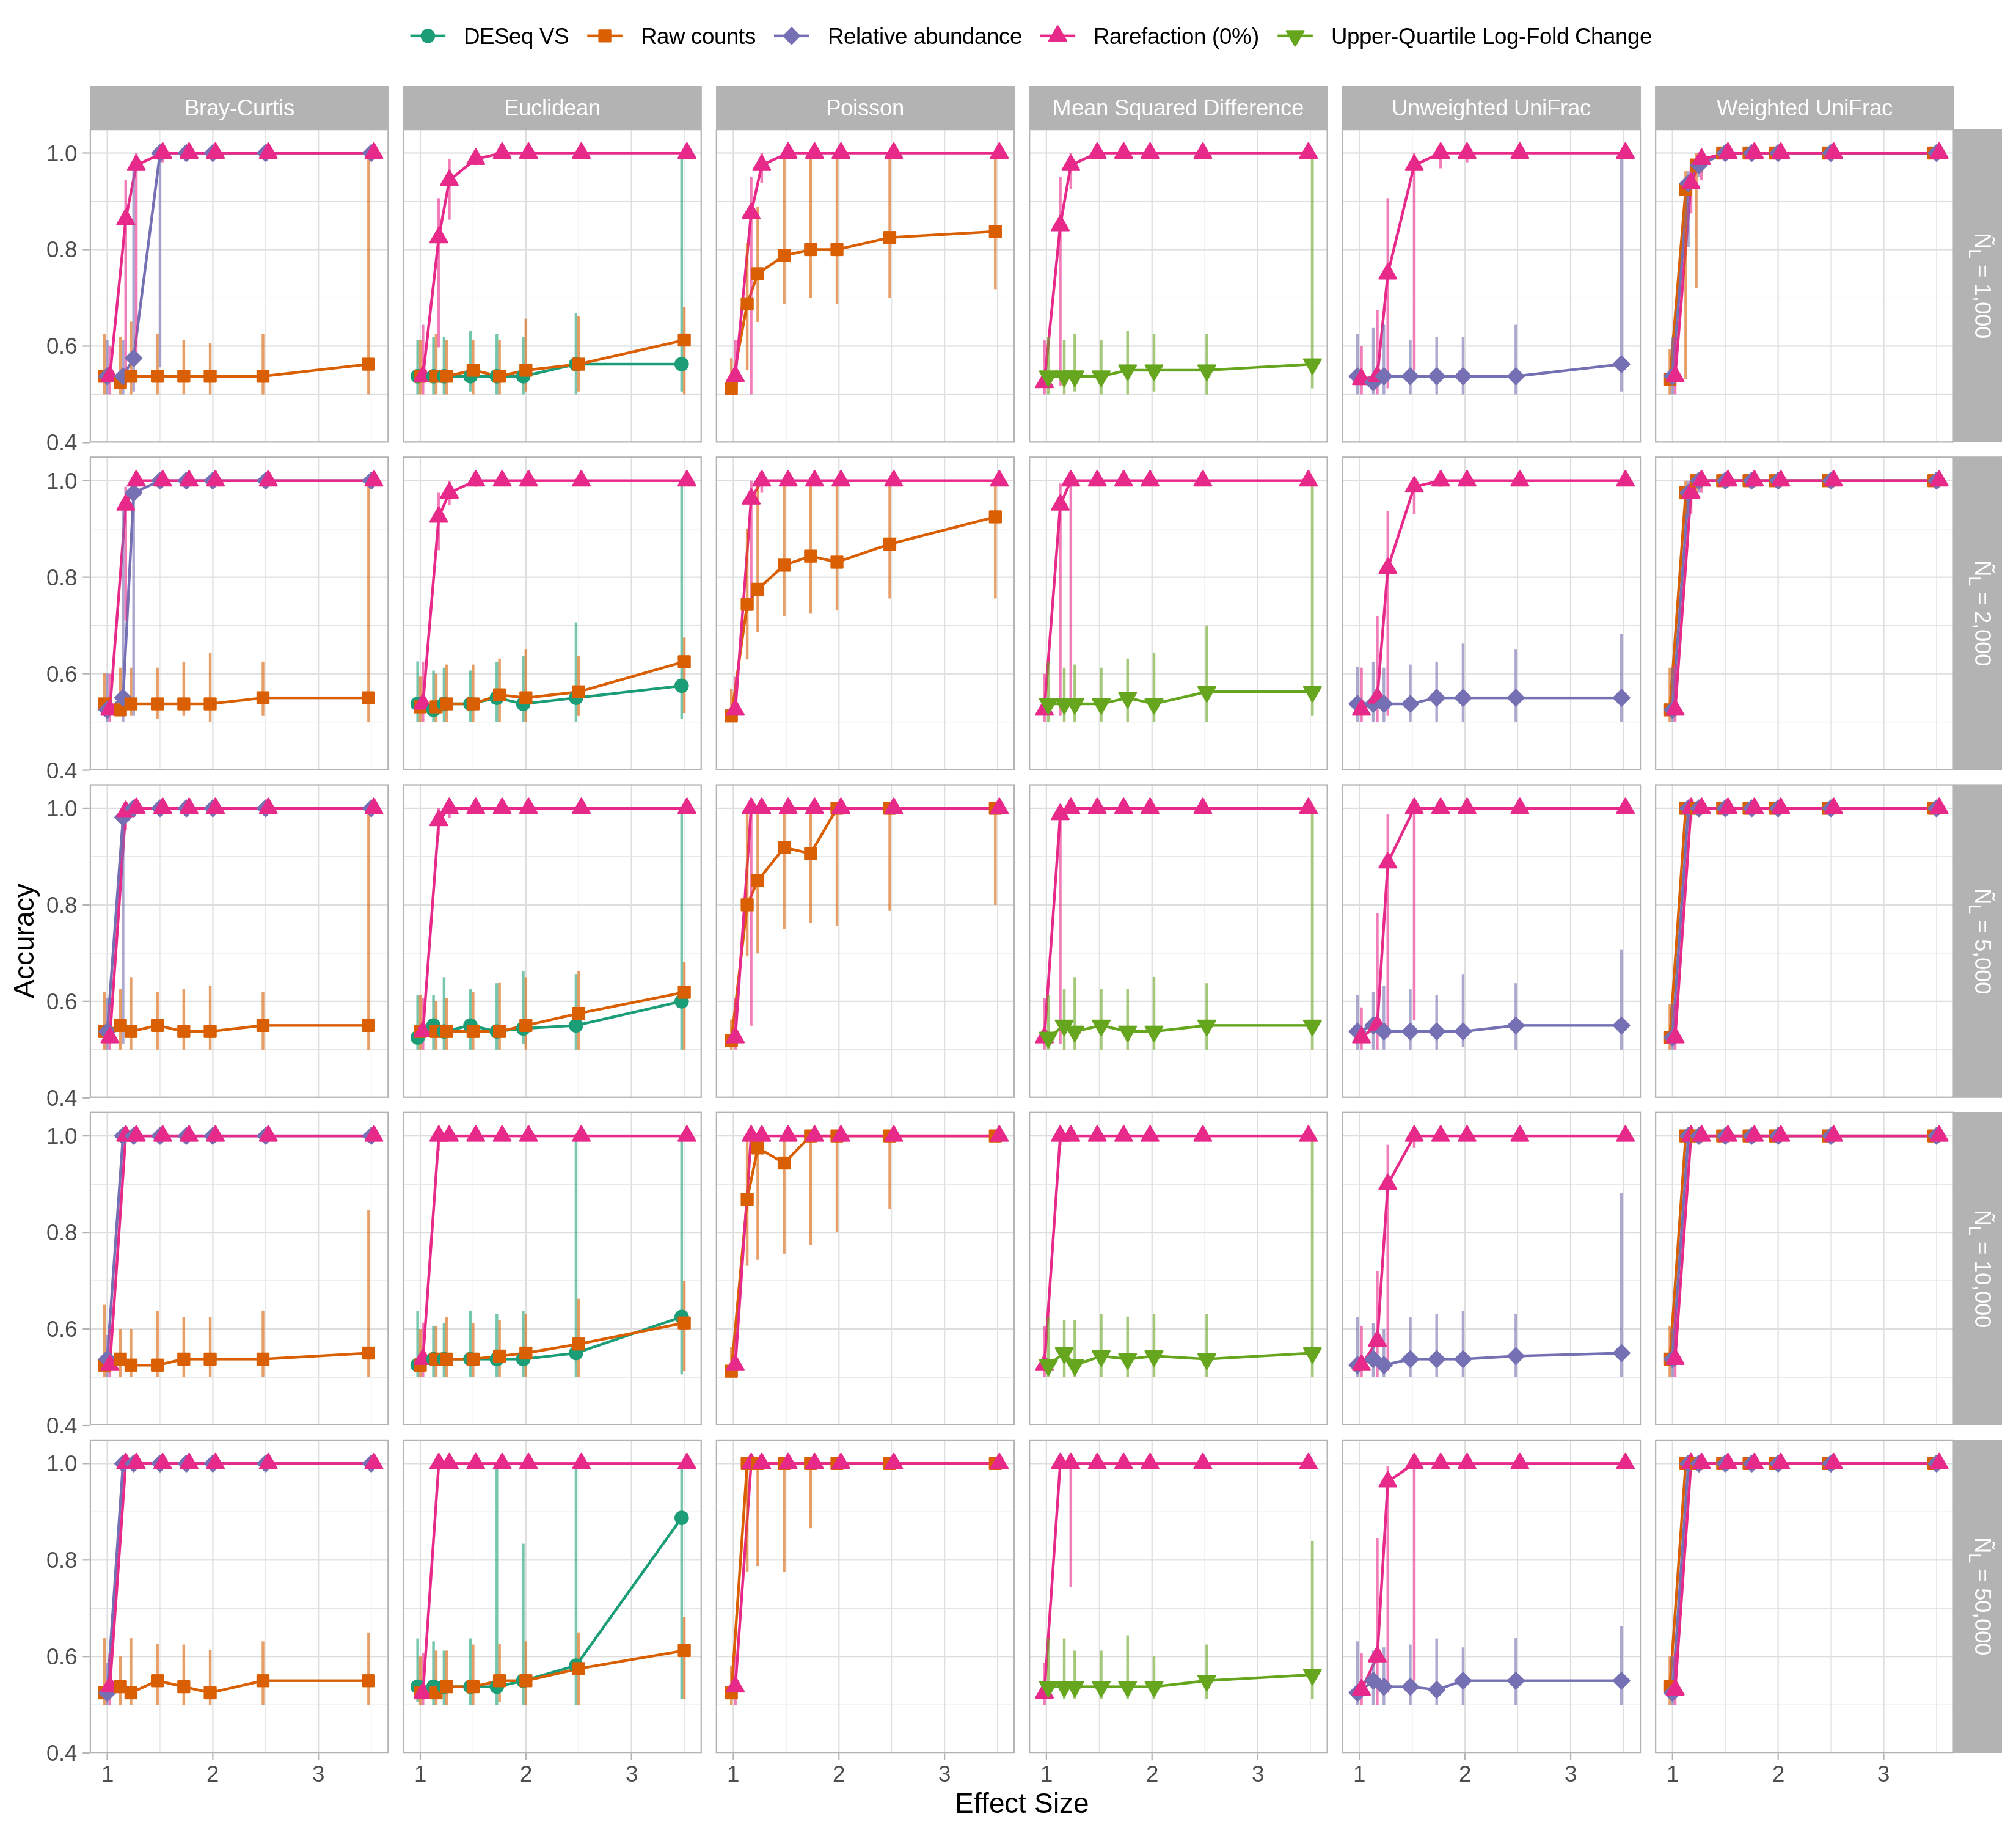
\includegraphics{figure_11.png}

\textbf{Figure 11. Clustering accuracies that used rarefaction were as
good or better than the other normalization procedures when a log-scaled
distribution of sequencing depths.} This figure is analogous to Figure 9
except that the sequencing depths for each of the 80 samples in each
simulation were drawn without replacement from a log-scaled distribution
rather than from the GlobalPatterns sequencing depths.

\newpage

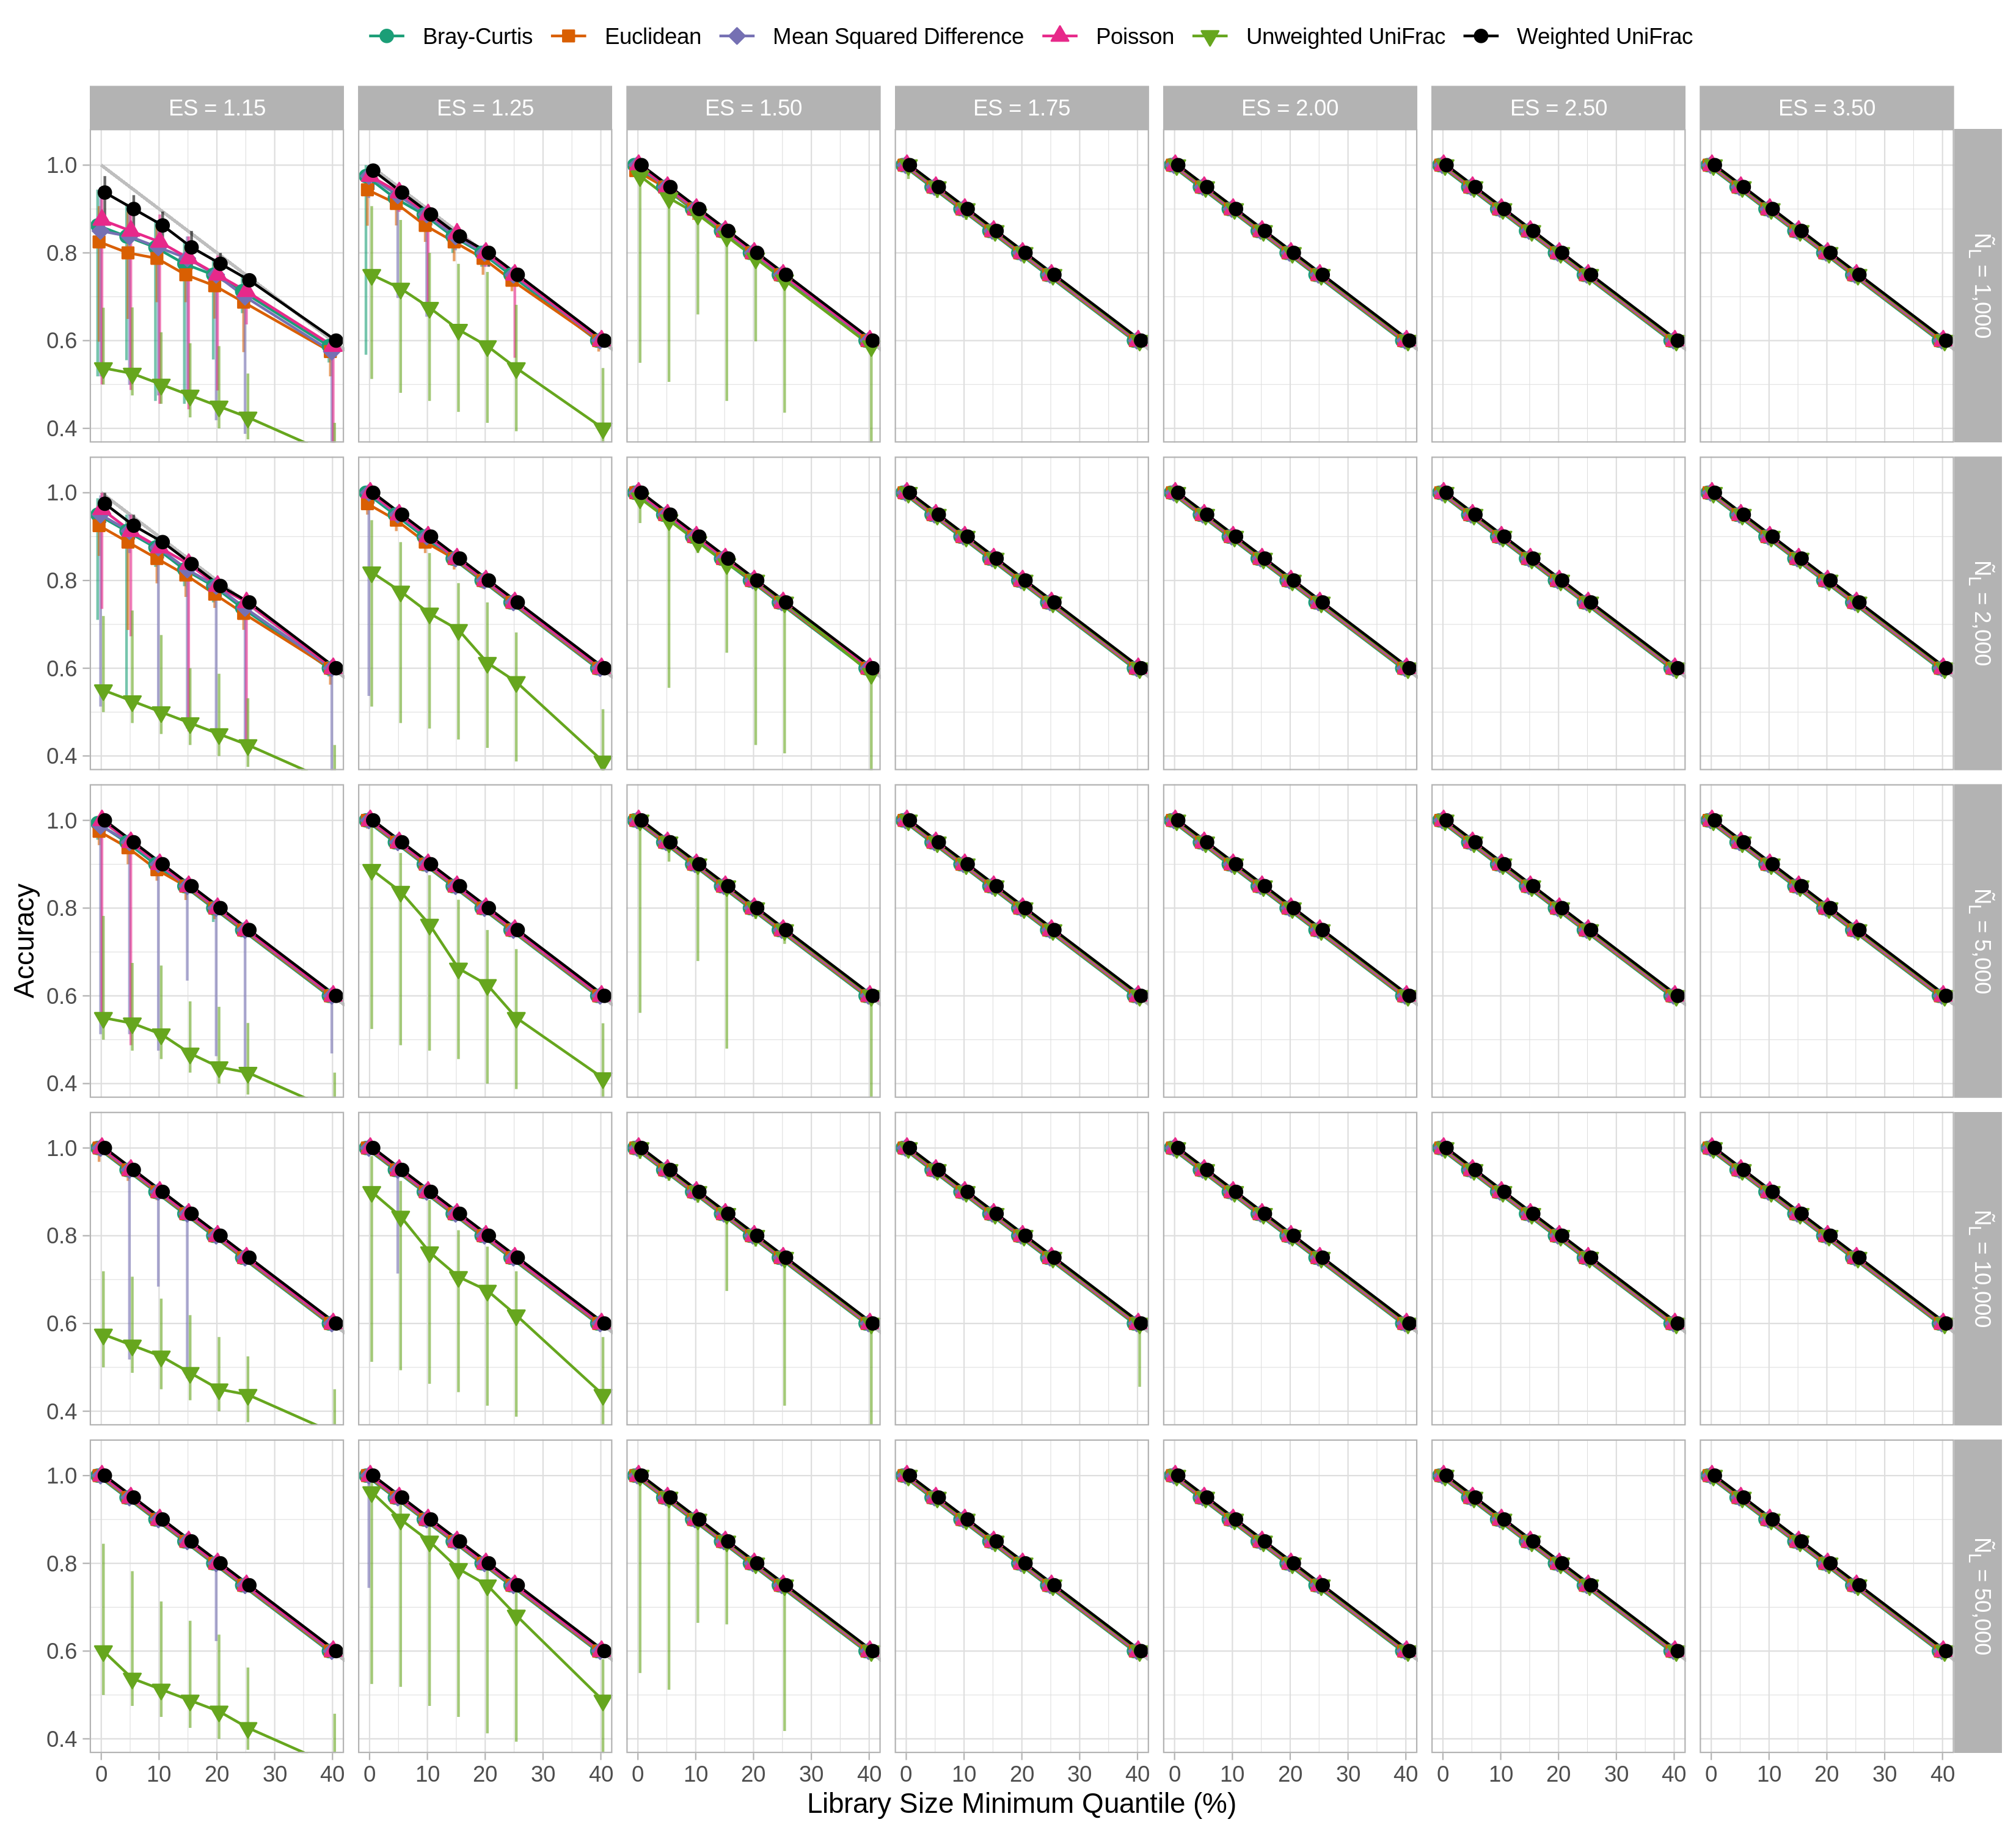
\includegraphics{figure_12.png}

\textbf{Figure 12. Rarefaction with all samples yielded clustering
accuracies that were as good or better than removing the smallest 15\%
of samples across distance calculation methods.} This figure is
analogous to Figure 8 except that the sequencing depths for each of the
80 samples in each simulation were drawn without replacement from a
log-scaled distribution rather than from the GlobalPatterns sequencing
depths.

\newpage

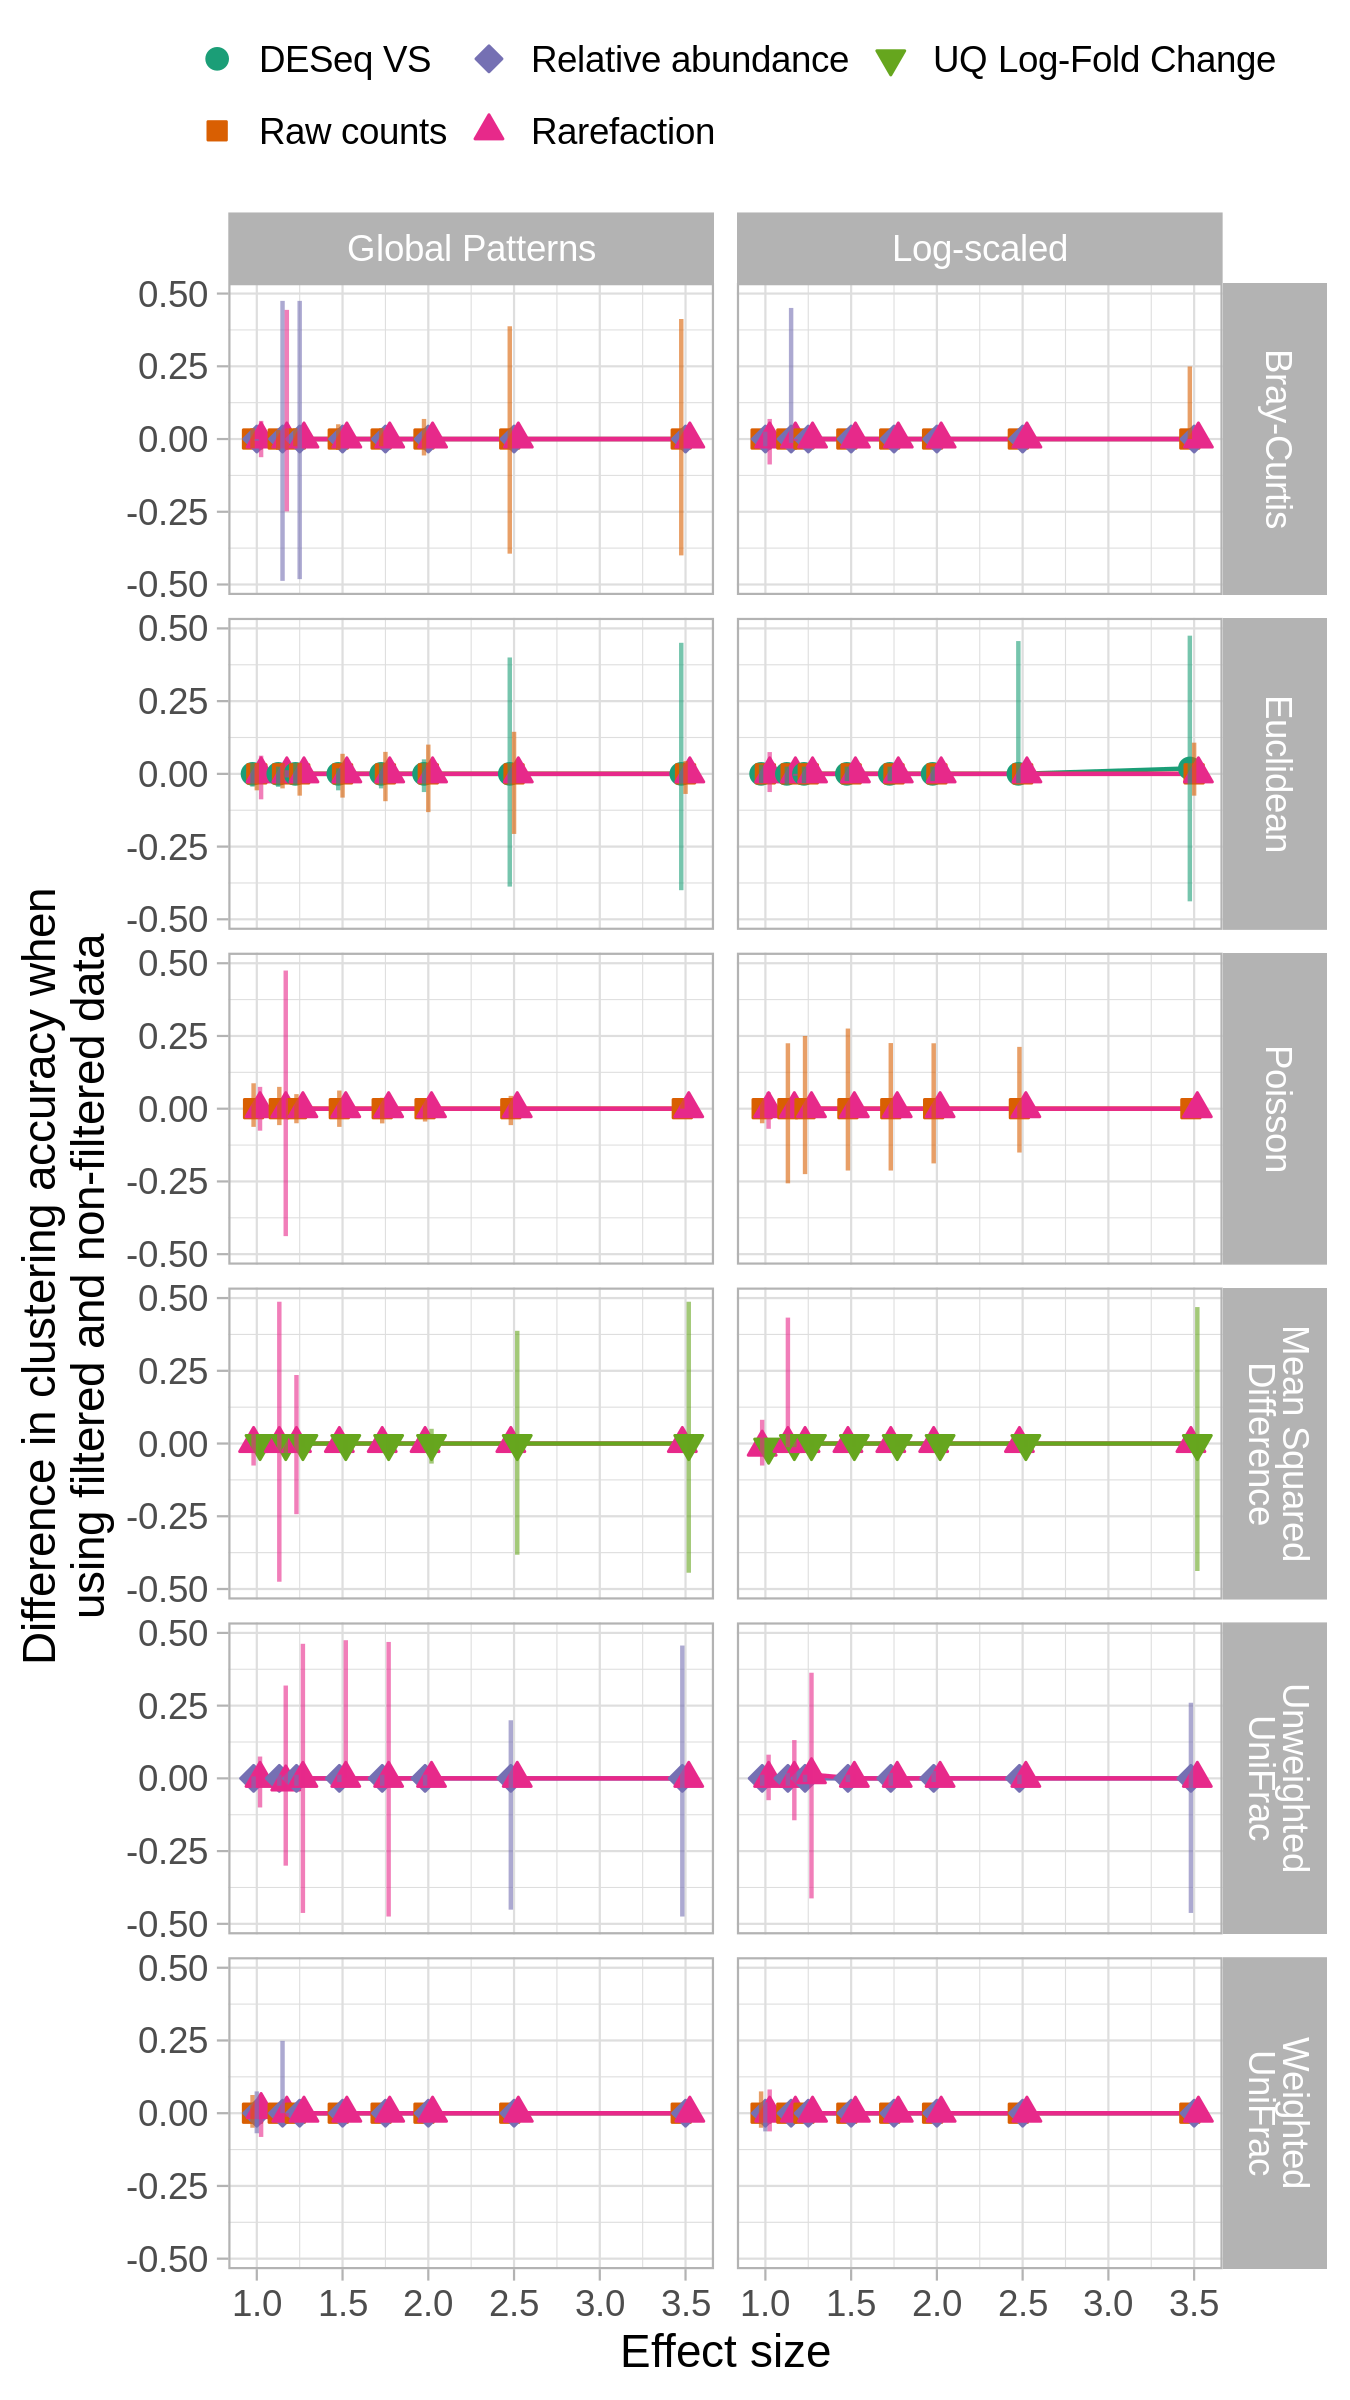
\includegraphics{figure_13.png}

\textbf{Figure 13. Normalization and distance calculation methods vary
in their sensitivity to removal of rare OTUs.} Larger values indicate
that the clustering accuracy from filtered datasets were larger than
those from non-filtered datasets. The median of 100 randomizations did
not meaningfully vary from 0.0, but the observed 95\% confidence
interval varied considerably. Data are shown for a median sequencing
depth (Ñ\textsubscript{L}) of 10,000 sequences when individual
sequencing depths were sampled with replacement from the GlobalPatterns
dataset or without replacement from the log-scaled distribution.

\newpage

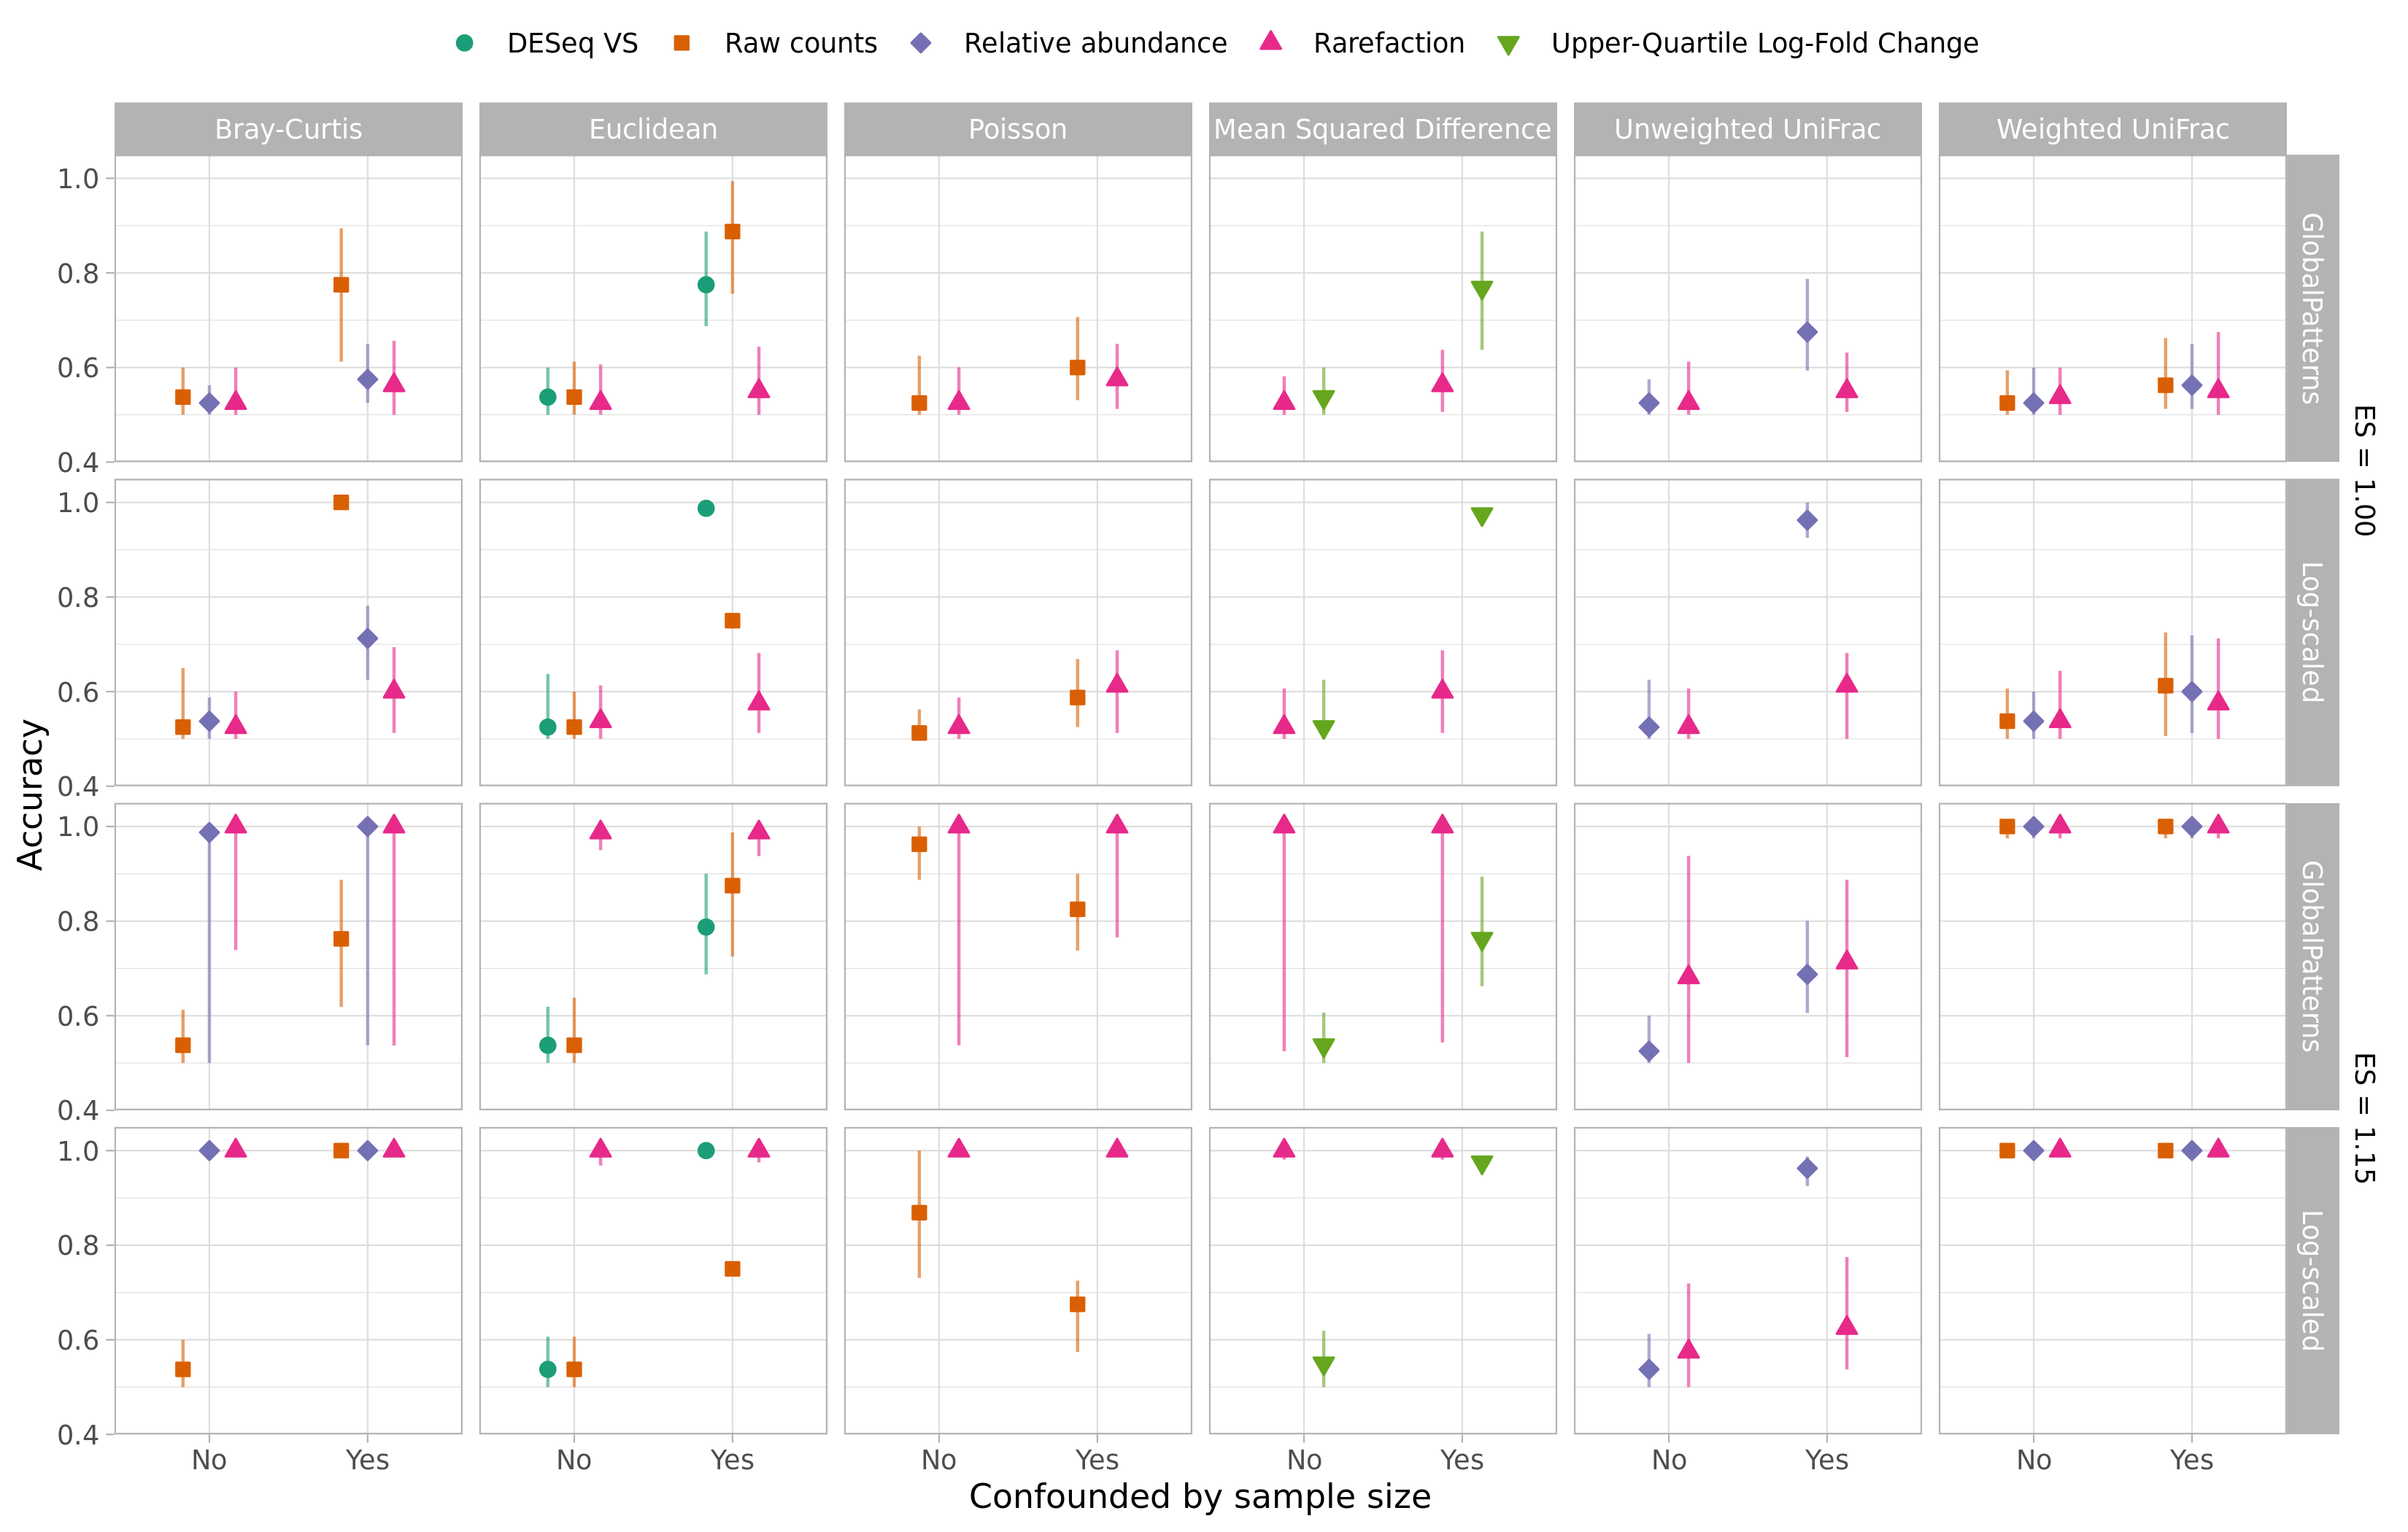
\includegraphics{figure_14.png}

\textbf{Figure 14. Rarefaction was consistently as good or better than
all other normalization methods at assigning samples to the correct
treatment group regardless of whether sequencing depth was confounded by
treatment group.} Because the clustering algorithms forced samples into
one of two groups, the expected accuracy with an effect size of 1.00 was
0.51. With an effect size of 1.15, the expected accuracy was 1.00. Each
point represents the median of 100 replicates and the error bars
represent the observed 95\% confidence interval. Data are shown for a
median sequencing depth (Ñ\textsubscript{L}) of 10,000 sequences when
individual sequencing depths were sampled with replacement from the
GlobalPatterns dataset or without replacement from the log-scaled
distribution.

\newpage

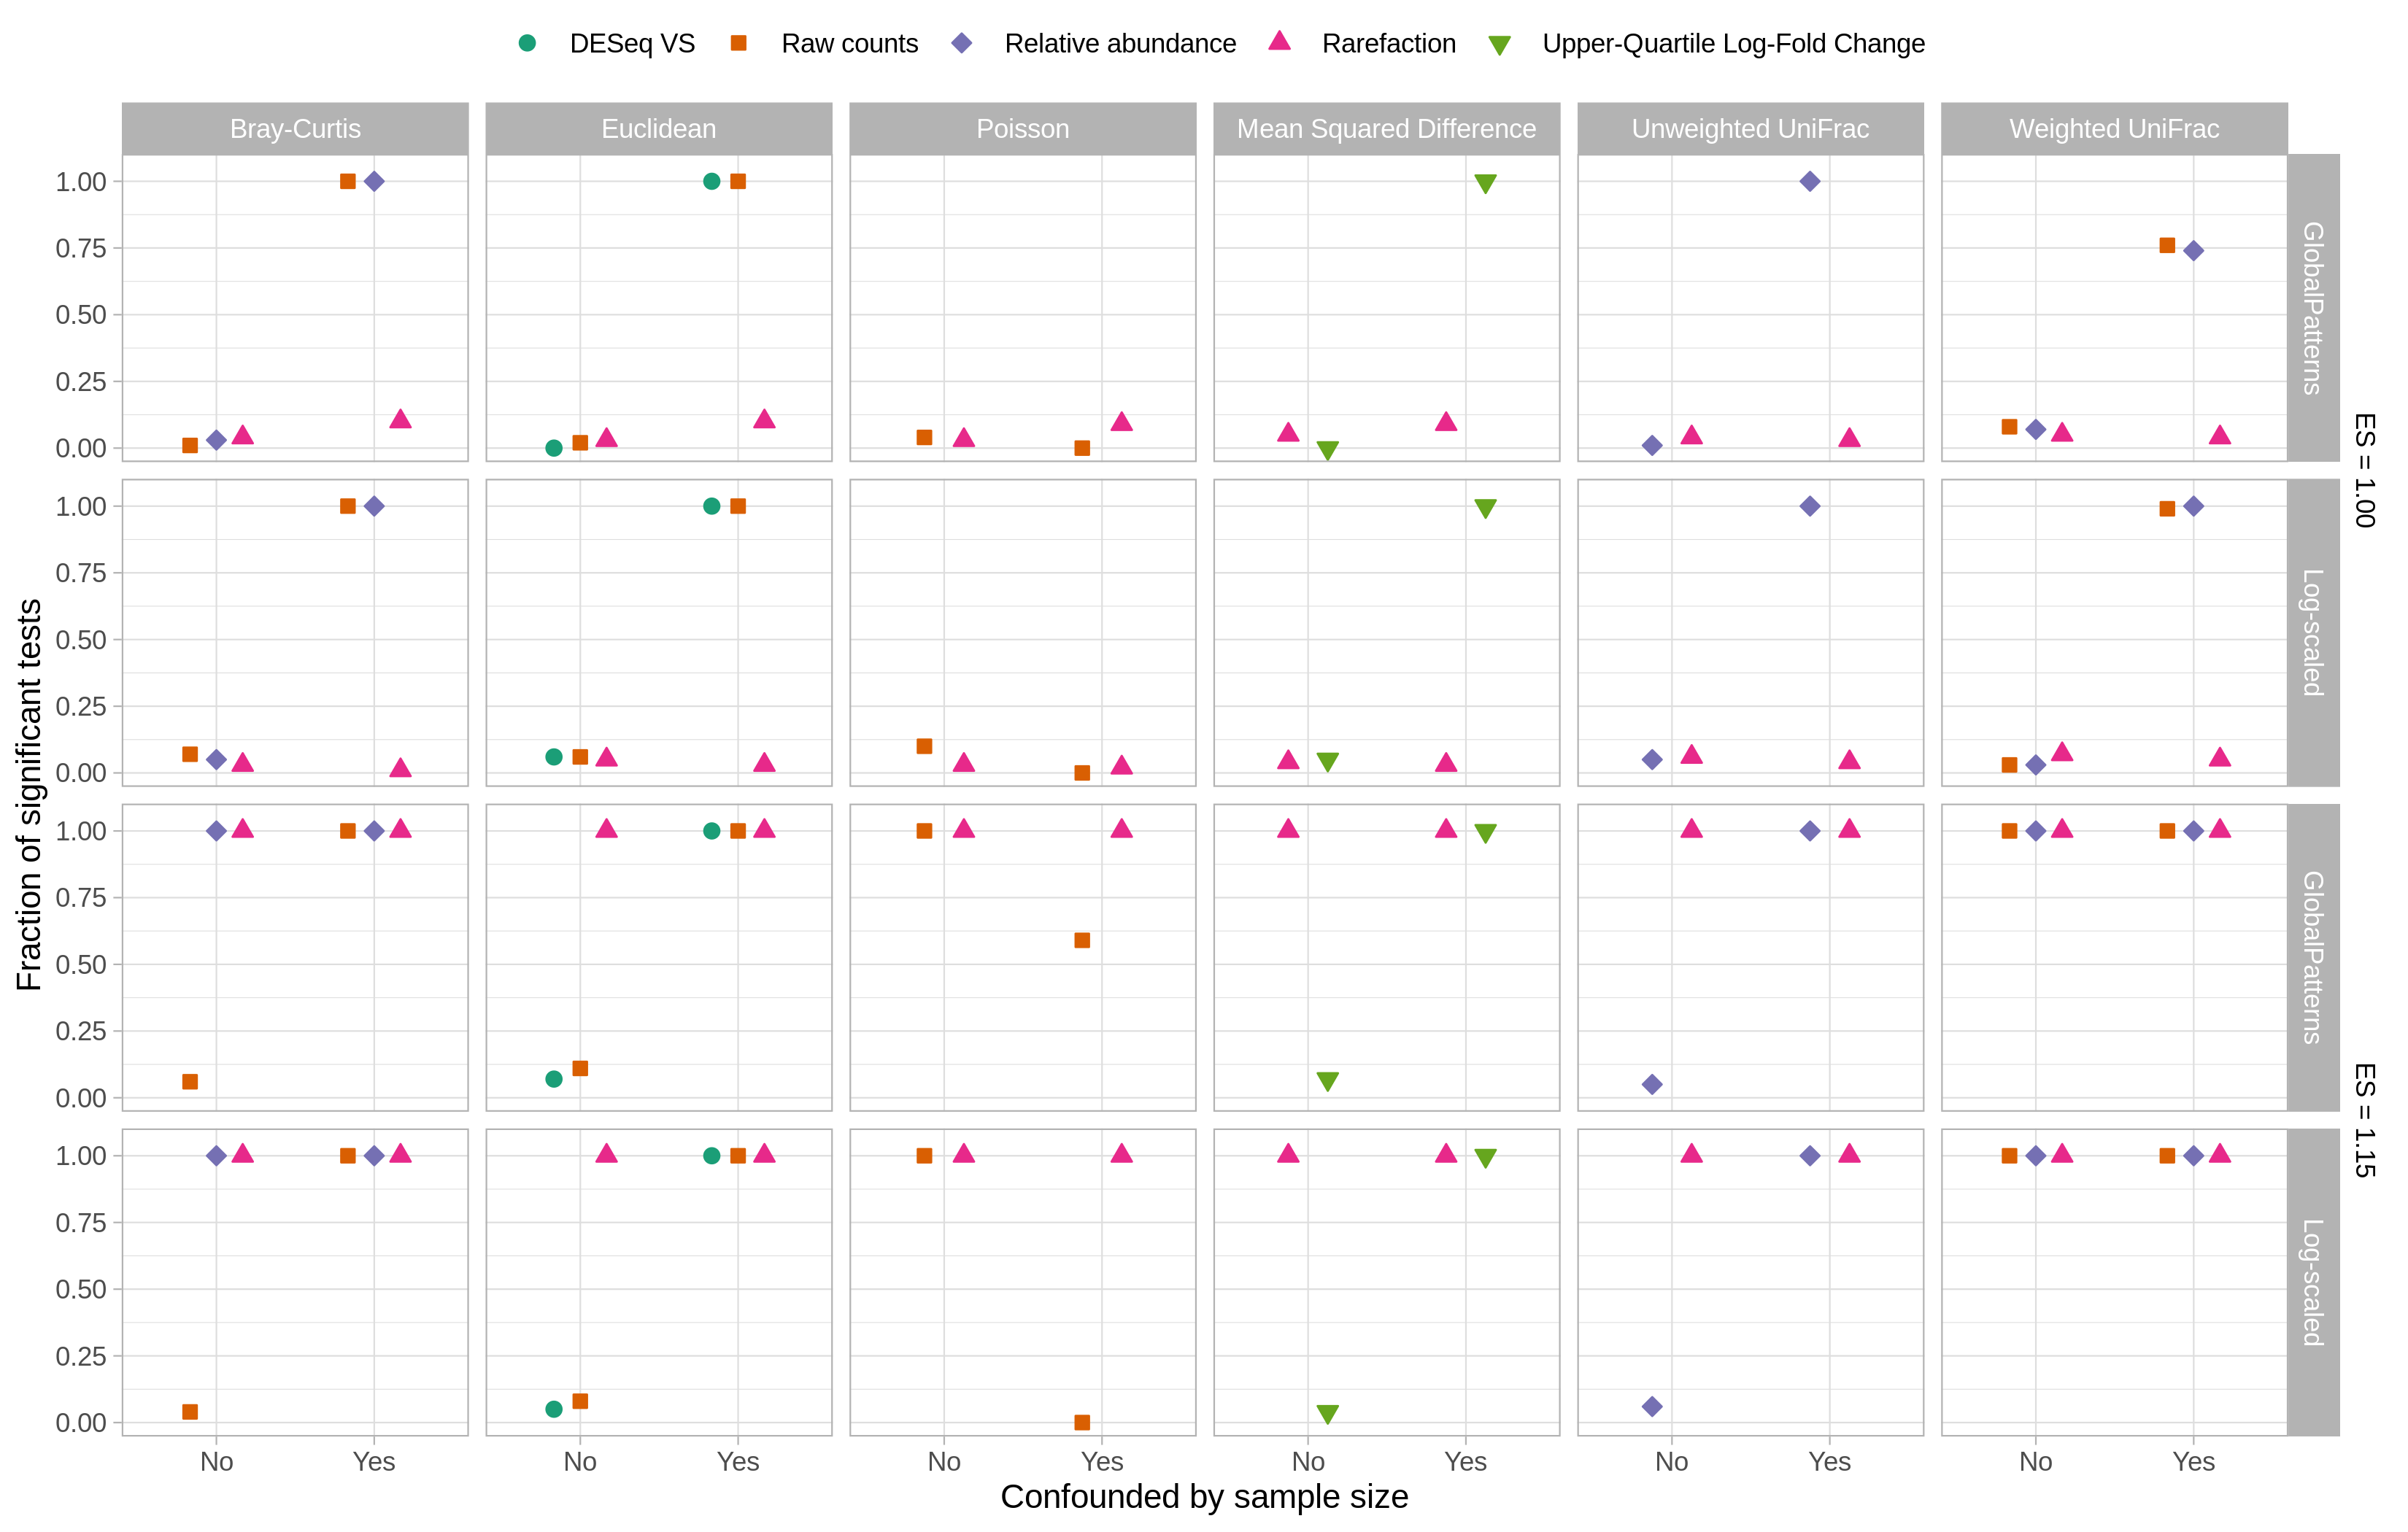
\includegraphics{figure_15.png}

\textbf{Figure 15. Rarefaction was consistently as good or better than
all other normalization methods at controlling for Type I error and
maximizing power to detect differences in treatment group using adonis2
regardless of whether sequencing depth was confounded by treatment
group.} Type I errors were assessed as the fraction of 100 simulations
that yielded a significant P-value (i.e., less than or equal to 0.05) at
an effect size of 1.00. Power was assessed as the fraction of 100
simulations that yielded a significant P-Value at an effect size of
1.15. Data are shown for a median sequencing depth (Ñ\textsubscript{L})
of 10,000 sequences when individual sequencing depths were sampled with
replacement from the GlobalPatterns dataset or without replacement from
the log-scaled distribution.

\newpage

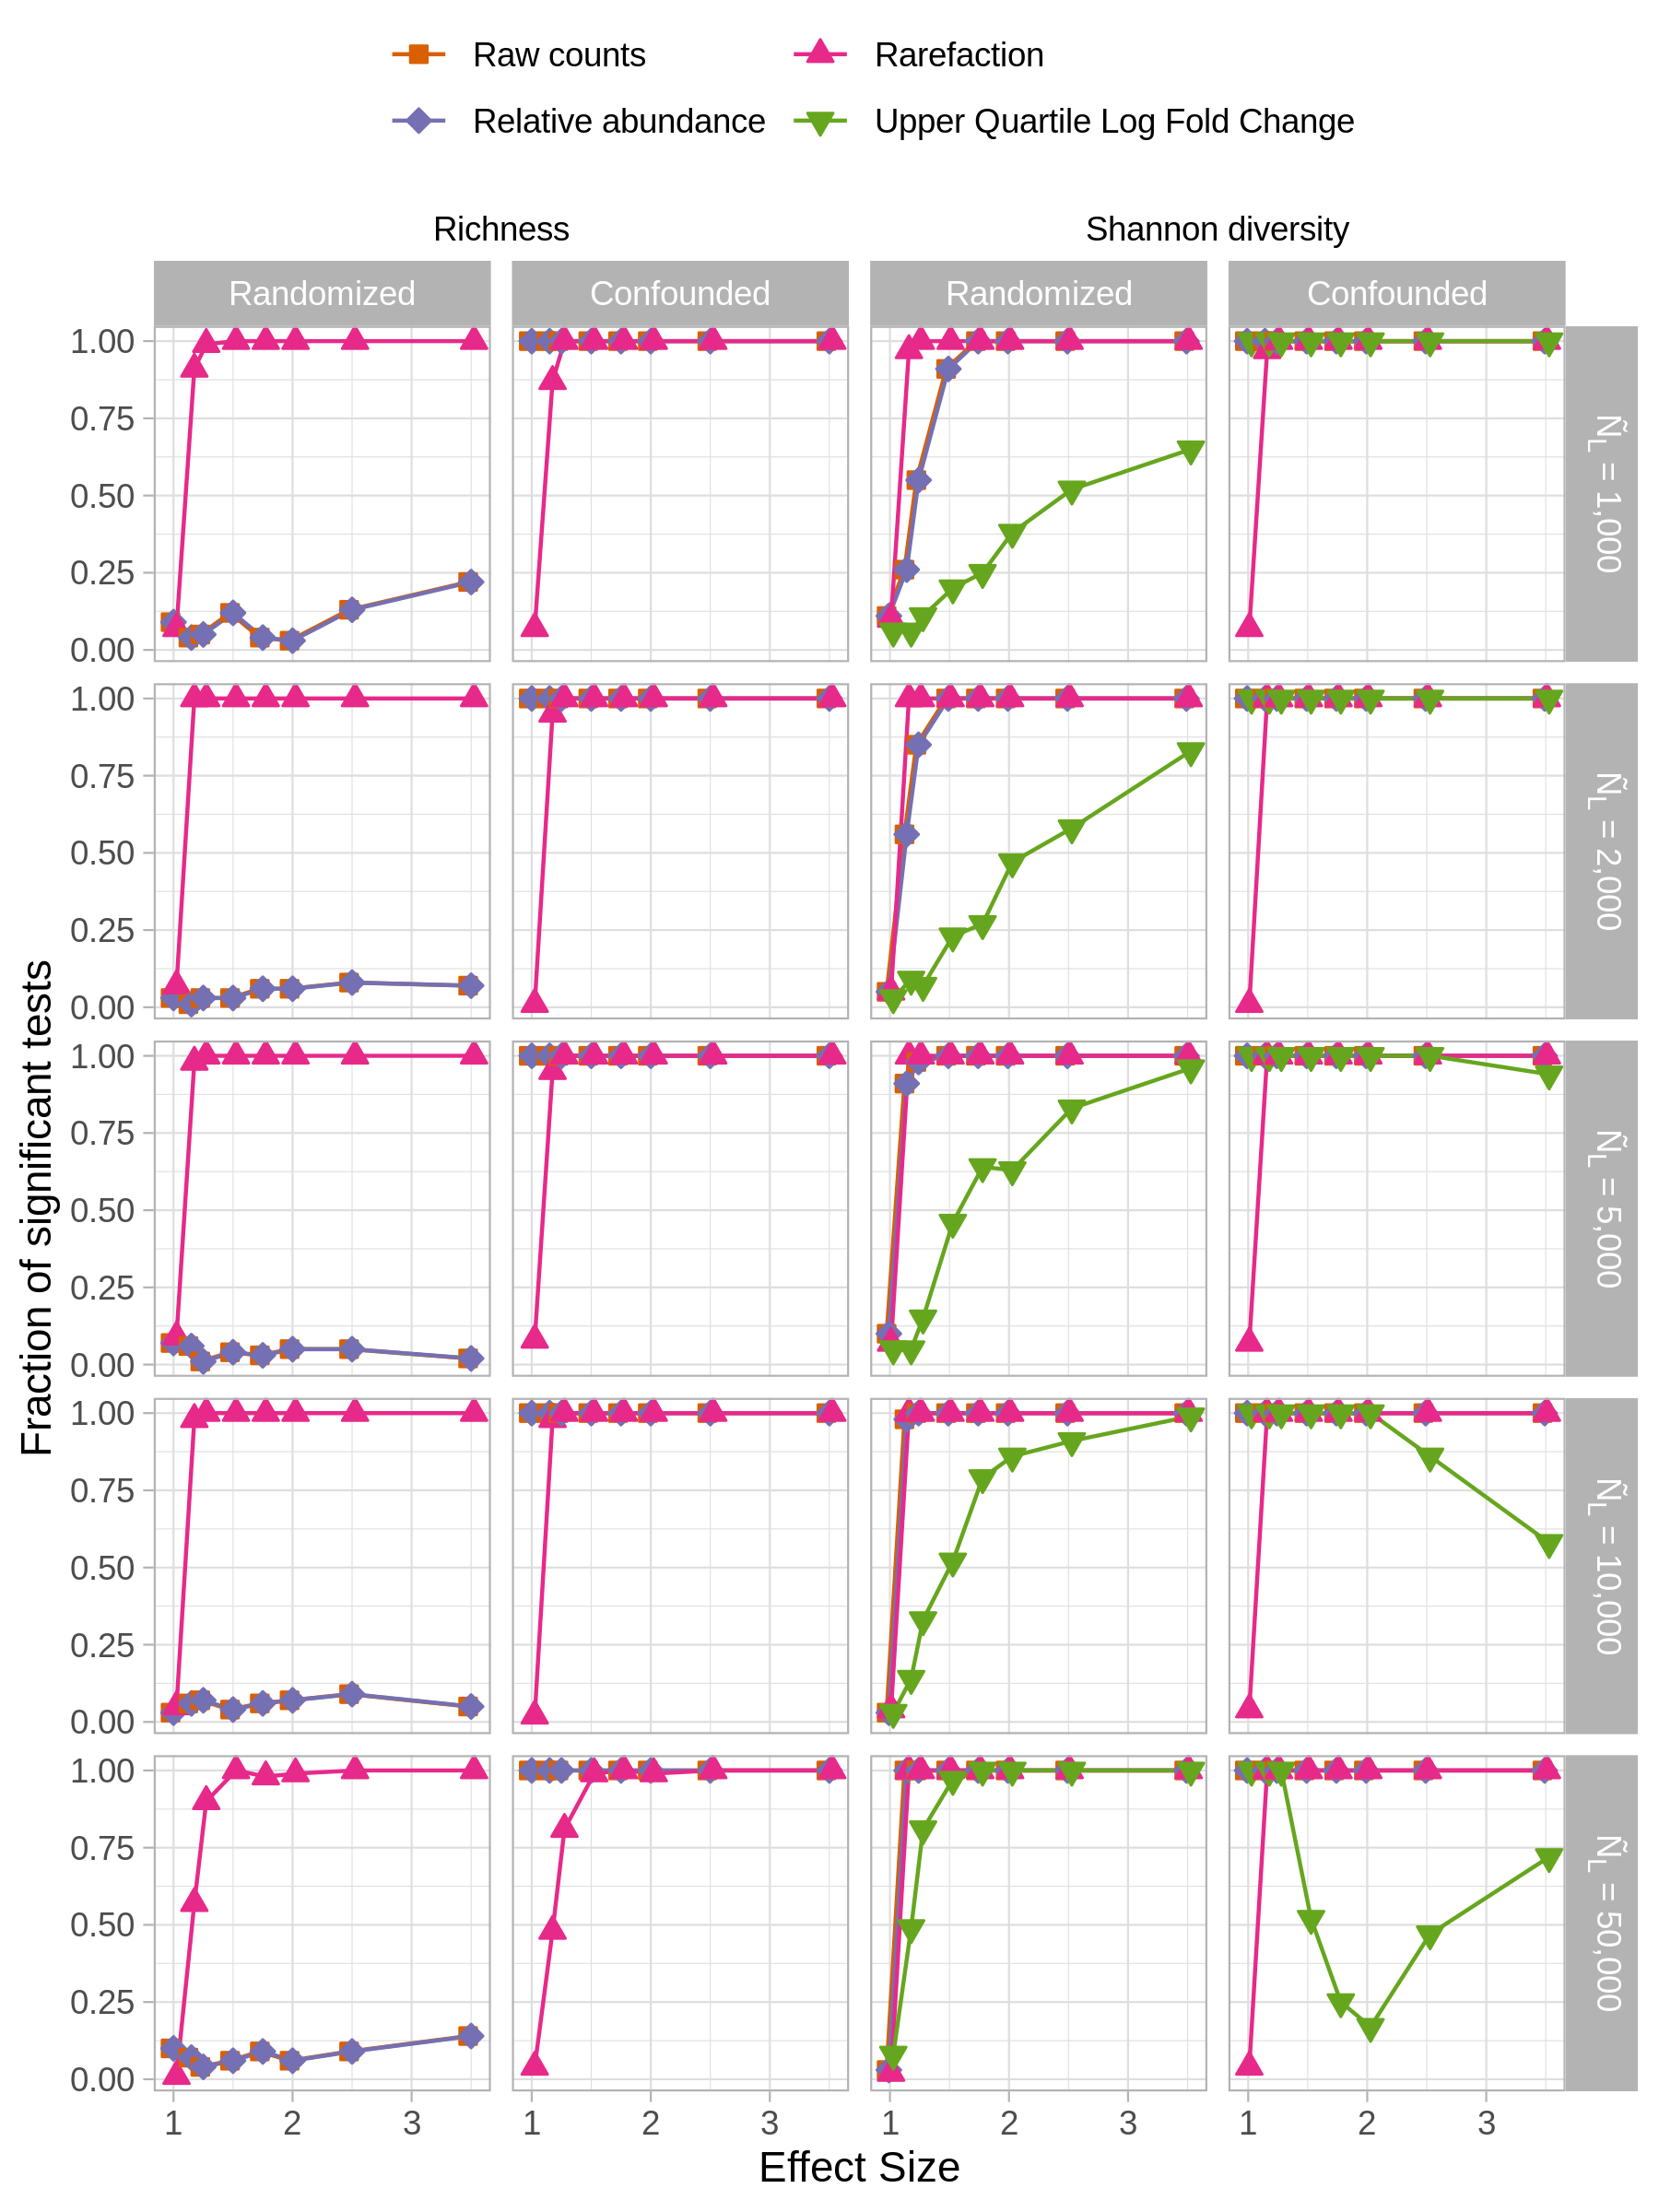
\includegraphics{figure_16.png}

\textbf{Figure 16. Rarefaction was consistently as good or better than
all other normalization methods at controlling for Type I error and
maximizing power to detect differences in treatment group using
alpha-diversity metrics regardless of whether sequencing depth was
confounded by treatment group.} Statistical comparisons of OTU richness
and Shannon diversity were performed using the non-parametric Wilcoxon
two-sampled test. Type I errors were assessed as the fraction of 100
simulations that yielded a significant P-value (i.e., less than or equal
to 0.05) at an effect size of 1.00. Power was assessed as the fraction
of 100 simulations that yielded a significant P-Value at an effect size
of 1.15. Data are shown for when the case when individual sequencing
depths were sampled with replacement from the GlobalPatterns dataset.

\newpage

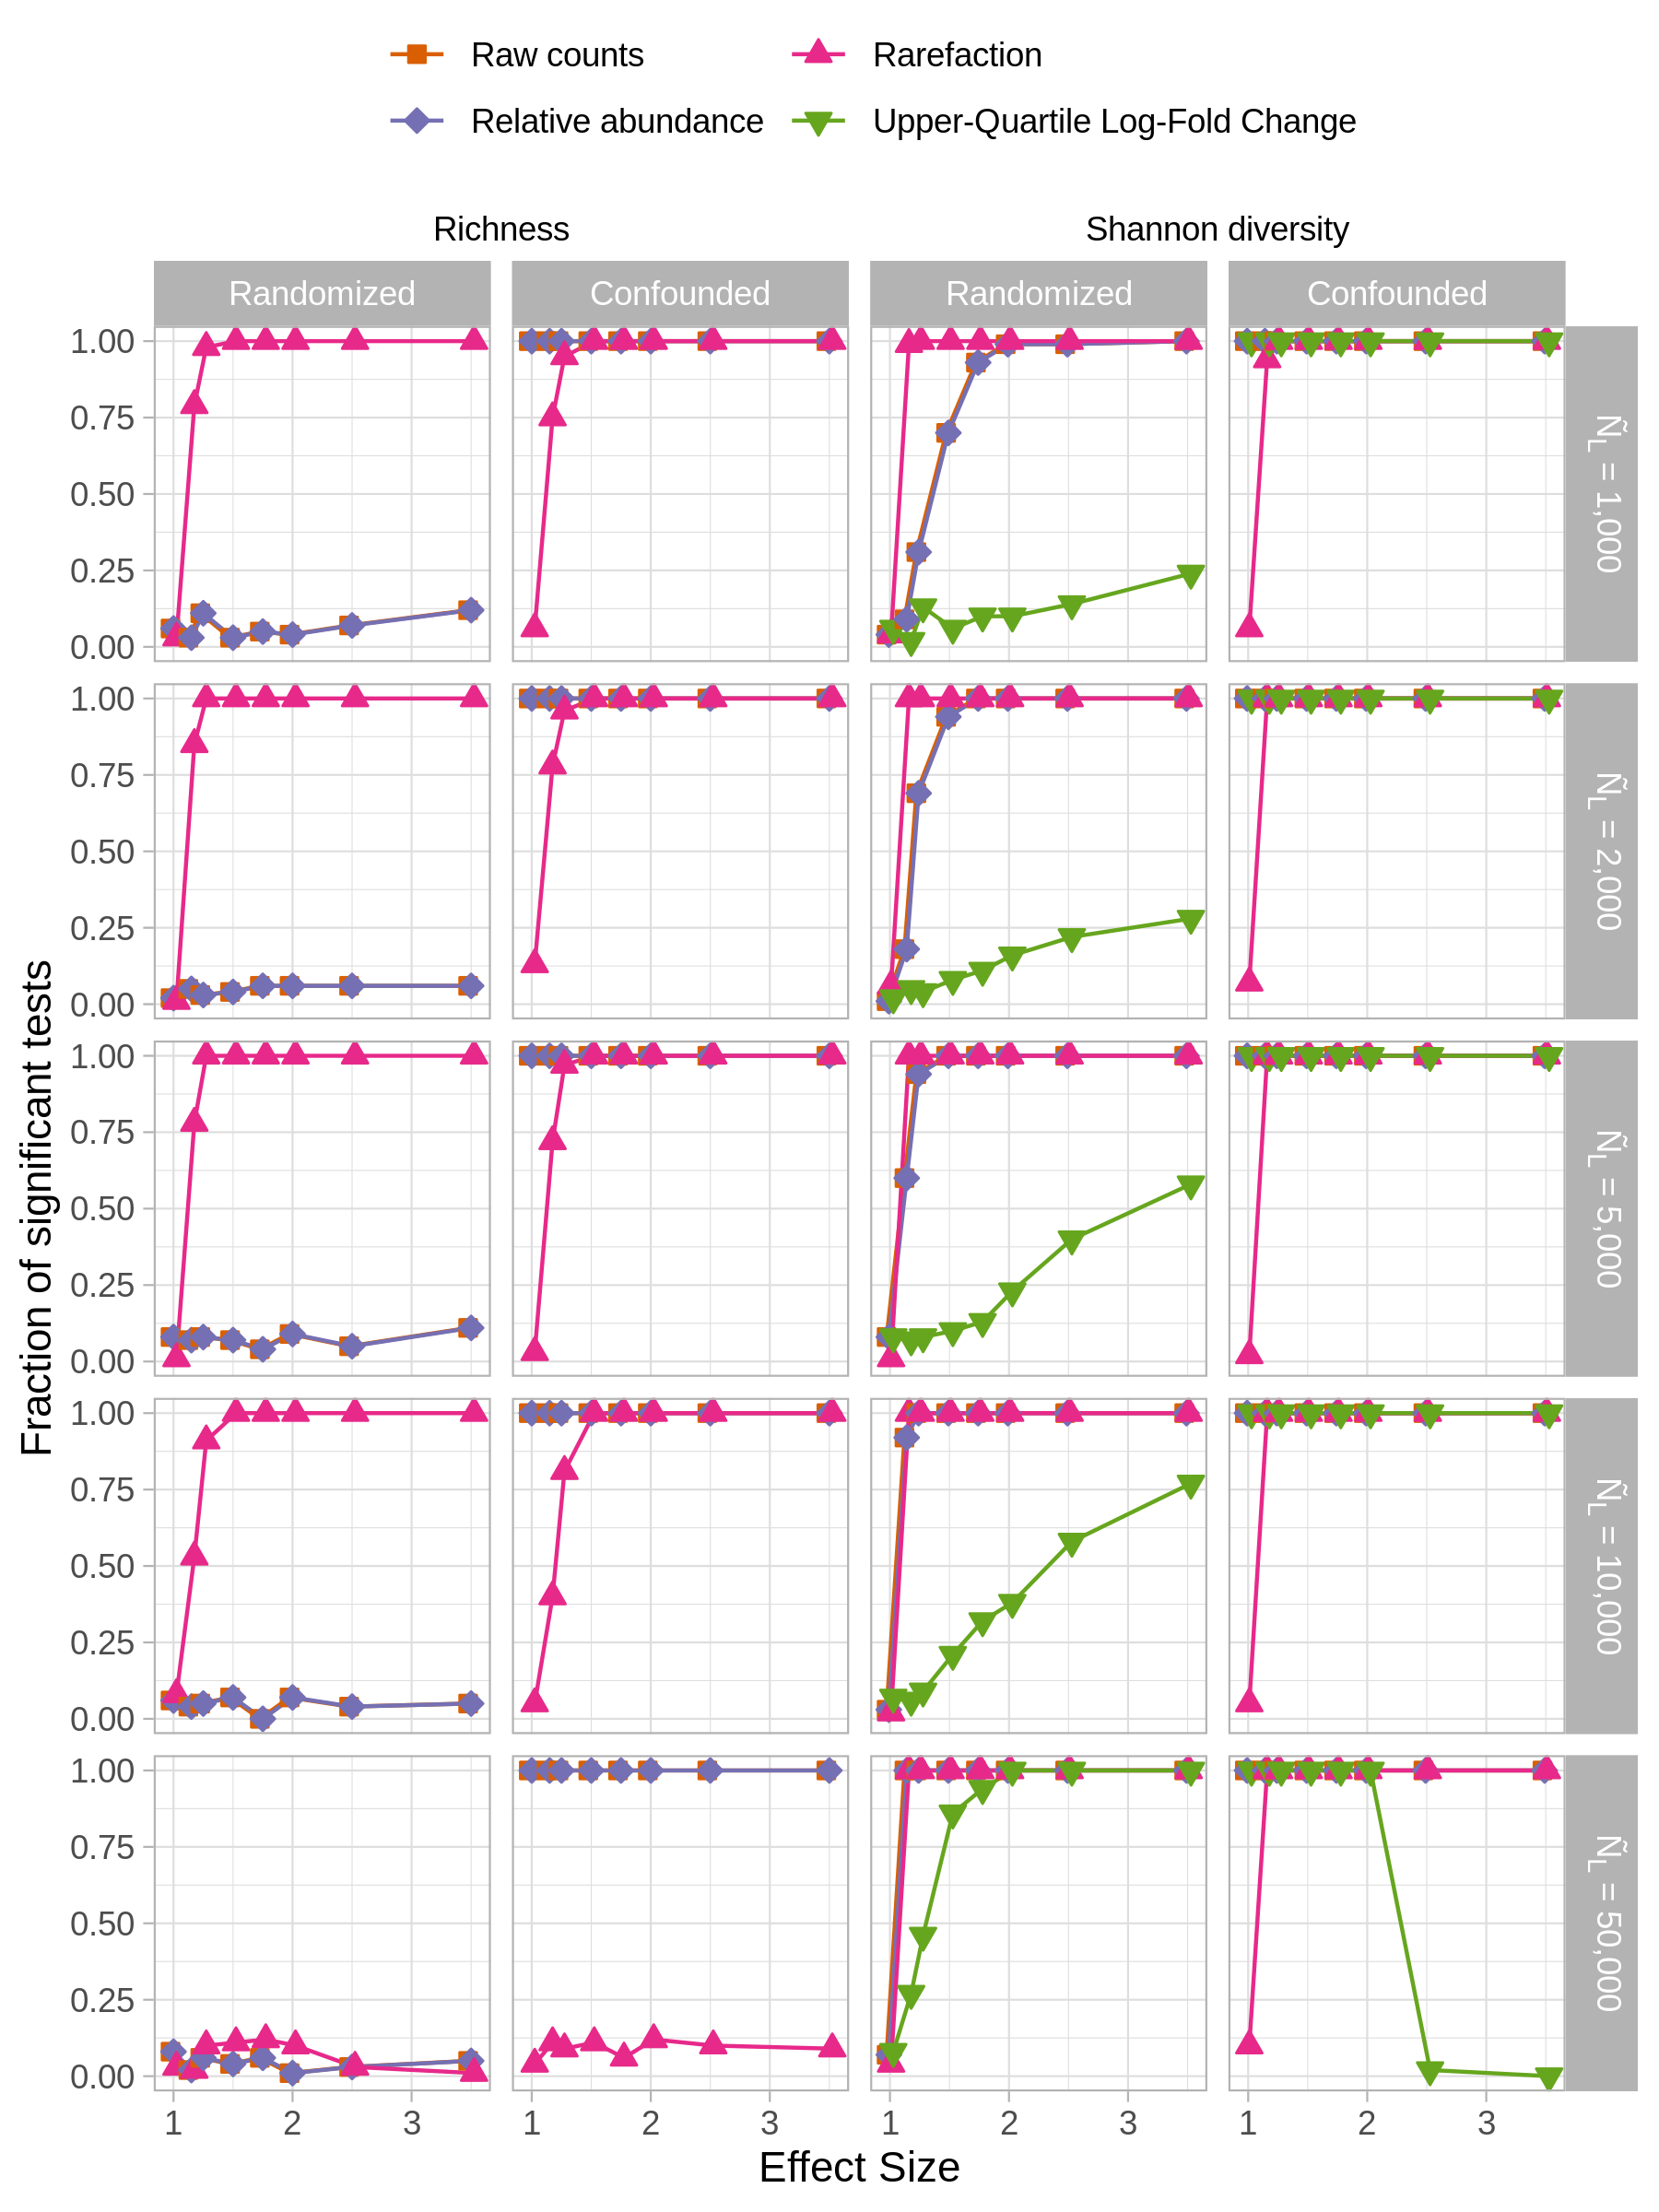
\includegraphics{figure_17.png}

\textbf{Figure 17. Rarefaction was consistently as good or better than
all other normalization methods at controlling for Type I error and
maximizing power to detect differences in treatment group using
alpha-diversity metrics regardless of whether sequencing depth was
confounded by treatment group.} Statistical comparisons of OTU richness
and Shannon diversity were performed using the non-parametric Wilcoxon
two-sampled test. Type I errors were assessed as the fraction of 100
simulations that yielded a significant P-value (i.e., less than or equal
to 0.05) at an effect size of 1.00. Power was assessed as the fraction
of 100 simulations that yielded a significant P-Value at an effect size
of 1.15. Data are shown for when the case when individual sequencing
depths were sampled without replacement from the log-scaled
distribution.

\newpage

\hypertarget{supplementary-text}{%
\subsection{Supplementary text}\label{supplementary-text}}

Quotes from selected papers that cited WNWN and conflated
``rarefying''/``rarefy'' and ``rarefaction''. Many of these papers also
attributed ``rarefaction'' to WNWN. Rarefying, rarefy, and rarefaction
are bolded to make the words easier to identify. All references have
been updated to reflect the numbering in the current study. Citations to
WNWN are indicated by (24). Quotes are ordered chronologically.

\begin{itemize}
\item
  ``Additionally, \textbf{rarefaction} has recently been shown to
  introduce errors in analyses, and alternatives to rarefaction have
  been proposed (24)'' - Quoted from (48). Implies that rarefaction and
  WNWN's rarefying are the same thing.
\item
  ``\textbf{Rarefaction} is analytically problematic and poses multiple
  statistical problems: (i) omission of available valid data, (ii) the
  estimation of overdispersion is more difficult due to data loss, (iii)
  loss of power (type II error), (iv) dependence on an arbitrary
  threshold and (v) additional uncertainty due to the randomness in
  \textbf{rarefaction} (24).'' - Quoted from (49). Implies that
  rarefaction and WNWN's rarefying are the same thing.
\item
  ``McMurdie and Holmes (24) penalized the \textbf{rarefying} technique
  for dropping the lowest fifteenth percentile of sample library sizes
  in their simulations by counting the dropped samples as''incorrectly
  clustered.'' Because the 15th percentile was used to set
  \textbf{rarefaction} depth, this capped clustering accuracy at 85\%.''
  - Quoted from (25). An example of a paper from the QIIME development
  community using rarefaction and rarefying interchangeably.
\item
  ``\textbf{Rarefaction} has a limited ability in this regard since the
  total sum constraint still exists after \textbf{rarefaction}. In
  addition, it suffers from a great power loss due to the discard of a
  large number of reads (24).'' - Quoted from (50). Implies that
  rarefaction and WNWN's rarefying are the same thing.
\item
  ``Another popular normalization approach is \textbf{rarefaction},
  which consists on subsampling the same number of reads for each sample
  so that all samples have the same number of total counts.
  \textbf{Rarefaction} is not recommended because it entails the loss of
  important information (24).'' - Quoted from (51). Implies that
  rarefaction and WNWN's rarefying are the same thing.
\item
  ``Unfortunately, \textbf{rarefaction} is neither justifiable nor
  necessary, a view framed statistically by McMurdie and Holmes (24) in
  the context of comparison of relative abundances.'' - Quoted from
  (21). Implies that rarefaction and WNWN's rarefying are the same
  thing.
\item
  ``Some studies perform \textbf{rarefaction} to adjust for differences
  in library size due to unexhaustive metagenomic sampling. Although
  several pipelines provide this functionality, it has been found
  inadmissible for metagenomics microbiome studies as it discards many
  reads leading to decreased sensitivity in differential abundance
  testing (24) and biased estimates for alpha diversity (21).'' - Quoted
  from (52). Implies that rarefaction and WNWN's rarefying are the same
  thing.
\item
  ``Another widespread practice is to \textbf{rarefy} the count data to
  force the samples to have the same number of total sequence reads
  (13), at the expense of discarding vast amounts of information (24).''
  - Quoted from (53). Hughes and Hellmann (13) describe traditional
  rarefaction with multiple subsamplings.
\item
  ``Note that the terms \textbf{rarefying} and \textbf{rarefaction} are
  used interchangeably in microbiome literature (24). \textbf{Rarefying}
  was first recommended for microbiome data to deal with rare taxa (54),
  which impact some measures of alpha and beta diversities (24).'' -
  Quoted from (14). As the quote indicates they use rarefying and
  rarefaction interchangeably although the cited WNWN indicates that
  they are not the same. In addition, the first review article to
  advocate the use of rarefaction was Hughes et al. (12) and examples of
  its use can be found earlier (55, 56);
\item
  ``Ways to tackle this include total library size normalization and
  \textbf{rarefaction}, with both remaining debated to date (24, 25).''
  - Quoted from (57). Implies that rarefaction and WNWN's rarefying are
  the same thing.
\item
  ``\textbf{Rarefaction} is a widely used normalization technique that
  involves the random subsampling of sequences from the initial sample
  library to a selected normalized library size. This process is often
  dismissed as statistically invalid because subsampling effectively
  discards a portion of the observed sequences, yet it remains prevalent
  in practice and the suitability of \textbf{rarefying}, relative to
  many other normalization approaches, for diversity analysis has been
  argued'' - Quoted by (30). Uses rarefaction and rarefying
  interchangeably. This paper describes a new method as ``repeated
  rarefying'', which is the traditional rarefaction approach.
\item
  ``Confronted with technical variation as well as the overall increase
  in raw sequencing data generated per sample over the years,
  \textbf{rarefaction} (or downsampling) was suggested to standardize
  within and across dataset comparisons \ldots{} However, sequencing
  depth-based downsizing procedures were soon criticized, not only for
  being wasteful and discarding information on low-abundant taxa (24),
  but also for being unsuited when applied to communities characterized
  by substantial variation in cell density (58).'' - Quoted by (59).
  Implies that rarefaction and WNWN's rarefying are the same thing.
\item
  ``Some have suggested that data should be \textbf{rarefied} (23, 25)
  to a common sampling depth, typically to the level of the sample with
  fewest sequences, while others argue that such \textbf{rarefaction} is
  `inadmissible' and favor approaches that transform or scale sequence
  counts (24, 47).'' - Quoted by (60). Uses rarefied and rarefaction
  interchangeably and implies that both are the same as WNWN's
  rarefying.
\item
  ``\textbf{Rarefaction} has been criticized for wasting data since we
  effectively remove a portion of the data in the downsampling procedure
  (24).'' - Quoted by (61). Here and elsewhere in this paper the authors
  use rarefaction and rarefying interchangeably and implies that both
  are the same as WNWN's rarefying.
\item
  ``\textbf{Rarefying} (also referred to as \textbf{rarefaction}) is a
  popular but widely criticized technique for correcting uneven
  sequencing depths. It involves randomly discarding counts in samples
  until all samples have the same predefined number of total counts.'' -
  Quoted by (62). As the quote indicates they use rarefying and
  rarefaction interchangeably although the cited WNWN indicates that
  they are not the same.
\item
  ``One commonly used method is to \textbf{rarefy} the data; that is,
  ASVs or OTUs within a sample are randomly subsampled without
  replacement to a preselected depth that is the same across all
  samples. The outcome of this is that all samples will have the same
  number of ASVs and any samples with fewer ASVs than the
  \textbf{rarefaction} level will be removed from the dataset. The level
  for \textbf{rarefaction} can be decided using a \textbf{rarefaction}
  curve, a method in which each sample is subsampled at multiple levels
  (e.g.~1,000 reads, 2,000 reads, 3,000 reads\ldots), and the number of
  unique features or another metric of individual sample diversity of
  each sample at each level is measured and plotted. When the plot
  begins to level off after an initial climb up, the corresponding
  number of sequences indicates an appropriate sampling depth. The
  appropriate number to \textbf{rarefy} must then be balanced with the
  number of samples that may be dropped from the dataset which do not
  meet that minimum. An advantage of \textbf{rarefaction} is that it may
  be a more appropriate measure of very low-abundance (''rare'') ASVs.
  This can in turn increase the accuracy of the data, as low biomass
  samples often have contamination and quality concerns (63). There are
  also disadvantages to this method, the most obvious of which is the
  discarding of valuable data. Clearly, this is less than ideal as the
  researcher must pay for the samples and sequences, and in cases where
  the samples are very valuable or difficult to obtain the loss of data
  may be destructive to the overall experimental integrity.
  Additionally, the loss of statistical power by removing sequences from
  a sample could lead to a loss of differences between two samples (24).
  The statistical consequences extend beyond this, as \textbf{rarefying}
  equalizes sample variance by adding artificial uncertainty (24).'' -
  Quoted by (64). The authors use rarefaction and rarefying
  interchangeably and implies that both are the same as WNWN's
  rarefying.
\end{itemize}

\end{document}
